\documentclass[twoside]{book}

% Packages required by doxygen
\usepackage{fixltx2e}
\usepackage{calc}
\usepackage{doxygen}
\usepackage[export]{adjustbox} % also loads graphicx
\usepackage{graphicx}
\usepackage[utf8]{inputenc}
\usepackage{makeidx}
\usepackage{multicol}
\usepackage{multirow}
\PassOptionsToPackage{warn}{textcomp}
\usepackage{textcomp}
\usepackage[nointegrals]{wasysym}
\usepackage[table]{xcolor}

% Font selection
\usepackage[T1]{fontenc}
\usepackage[scaled=.90]{helvet}
\usepackage{courier}
\usepackage{amssymb}
\usepackage{sectsty}
\renewcommand{\familydefault}{\sfdefault}
\allsectionsfont{%
  \fontseries{bc}\selectfont%
  \color{darkgray}%
}
\renewcommand{\DoxyLabelFont}{%
  \fontseries{bc}\selectfont%
  \color{darkgray}%
}
\newcommand{\+}{\discretionary{\mbox{\scriptsize$\hookleftarrow$}}{}{}}

% Page & text layout
\usepackage{geometry}
\geometry{%
  a4paper,%
  top=2.5cm,%
  bottom=2.5cm,%
  left=2.5cm,%
  right=2.5cm%
}
\tolerance=750
\hfuzz=15pt
\hbadness=750
\setlength{\emergencystretch}{15pt}
\setlength{\parindent}{0cm}
\setlength{\parskip}{3ex plus 2ex minus 2ex}
\makeatletter
\renewcommand{\paragraph}{%
  \@startsection{paragraph}{4}{0ex}{-1.0ex}{1.0ex}{%
    \normalfont\normalsize\bfseries\SS@parafont%
  }%
}
\renewcommand{\subparagraph}{%
  \@startsection{subparagraph}{5}{0ex}{-1.0ex}{1.0ex}{%
    \normalfont\normalsize\bfseries\SS@subparafont%
  }%
}
\makeatother

% Headers & footers
\usepackage{fancyhdr}
\pagestyle{fancyplain}
\fancyhead[LE]{\fancyplain{}{\bfseries\thepage}}
\fancyhead[CE]{\fancyplain{}{}}
\fancyhead[RE]{\fancyplain{}{\bfseries\leftmark}}
\fancyhead[LO]{\fancyplain{}{\bfseries\rightmark}}
\fancyhead[CO]{\fancyplain{}{}}
\fancyhead[RO]{\fancyplain{}{\bfseries\thepage}}
\fancyfoot[LE]{\fancyplain{}{}}
\fancyfoot[CE]{\fancyplain{}{}}
\fancyfoot[RE]{\fancyplain{}{\bfseries\scriptsize Generated by Doxygen }}
\fancyfoot[LO]{\fancyplain{}{\bfseries\scriptsize Generated by Doxygen }}
\fancyfoot[CO]{\fancyplain{}{}}
\fancyfoot[RO]{\fancyplain{}{}}
\renewcommand{\footrulewidth}{0.4pt}
\renewcommand{\chaptermark}[1]{%
  \markboth{#1}{}%
}
\renewcommand{\sectionmark}[1]{%
  \markright{\thesection\ #1}%
}

% Indices & bibliography
\usepackage{natbib}
\usepackage[titles]{tocloft}
\setcounter{tocdepth}{3}
\setcounter{secnumdepth}{5}
\makeindex

% Hyperlinks (required, but should be loaded last)
\usepackage{ifpdf}
\ifpdf
  \usepackage[pdftex,pagebackref=true]{hyperref}
\else
  \usepackage[ps2pdf,pagebackref=true]{hyperref}
\fi
\hypersetup{%
  colorlinks=true,%
  linkcolor=blue,%
  citecolor=blue,%
  unicode%
}

% Custom commands
\newcommand{\clearemptydoublepage}{%
  \newpage{\pagestyle{empty}\cleardoublepage}%
}

\usepackage{caption}
\captionsetup{labelsep=space,justification=centering,font={bf},singlelinecheck=off,skip=4pt,position=top}

%===== C O N T E N T S =====

\begin{document}

% Titlepage & ToC
\hypersetup{pageanchor=false,
             bookmarksnumbered=true,
             pdfencoding=unicode
            }
\pagenumbering{alph}
\begin{titlepage}
\vspace*{7cm}
\begin{center}%
{\Large L\+I\+VE Tool HvA }\\
\vspace*{1cm}
{\large Generated by Doxygen 1.8.13}\\
\end{center}
\end{titlepage}
\clearemptydoublepage
\pagenumbering{roman}
\tableofcontents
\clearemptydoublepage
\pagenumbering{arabic}
\hypersetup{pageanchor=true}

%--- Begin generated contents ---
\chapter{Hierarchical Index}
\section{Class Hierarchy}
This inheritance list is sorted roughly, but not completely, alphabetically\+:\begin{DoxyCompactList}
\item Checking\begin{DoxyCompactList}
\item \contentsline{section}{Model\+Controller}{\pageref{class_model_controller}}{}
\item \contentsline{section}{Open\+File\+Script}{\pageref{class_open_file_script}}{}
\end{DoxyCompactList}
\item Mono\+Behaviour\begin{DoxyCompactList}
\item \contentsline{section}{Close\+Tab}{\pageref{class_close_tab}}{}
\item \contentsline{section}{Console\+Script}{\pageref{class_console_script}}{}
\item \contentsline{section}{Definition\+Script}{\pageref{class_definition_script}}{}
\item \contentsline{section}{Dynamic\+Tab}{\pageref{class_dynamic_tab}}{}
\item \contentsline{section}{Edge\+Inspector}{\pageref{class_edge_inspector}}{}
\item \contentsline{section}{Editor\+Button\+Script}{\pageref{class_editor_button_script}}{}
\item \contentsline{section}{Event\+Manager}{\pageref{class_event_manager}}{}
\item \contentsline{section}{Exit\+Button}{\pageref{class_exit_button}}{}
\item \contentsline{section}{Export\+File\+Script}{\pageref{class_export_file_script}}{}
\item \contentsline{section}{Model\+Controller}{\pageref{class_model_controller}}{}
\item \contentsline{section}{Model\+View\+Controller}{\pageref{class_model_view_controller}}{}
\item \contentsline{section}{Node\+Inspector}{\pageref{class_node_inspector}}{}
\item \contentsline{section}{Open\+File\+Script}{\pageref{class_open_file_script}}{}
\item \contentsline{section}{Select\+Edge\+Button}{\pageref{class_select_edge_button}}{}
\item \contentsline{section}{Select\+Node\+Button}{\pageref{class_select_node_button}}{}
\item \contentsline{section}{Tab\+Manager}{\pageref{class_tab_manager}}{}
\item \contentsline{section}{Tab\+Text}{\pageref{class_tab_text}}{}
\item \contentsline{section}{Toggle\+Tool}{\pageref{class_toggle_tool}}{}
\item \contentsline{section}{Zoom\+Content\+Script}{\pageref{class_zoom_content_script}}{}
\end{DoxyCompactList}
\item Parsing\begin{DoxyCompactList}
\item \contentsline{section}{Model\+Controller}{\pageref{class_model_controller}}{}
\item \contentsline{section}{Open\+File\+Script}{\pageref{class_open_file_script}}{}
\end{DoxyCompactList}
\end{DoxyCompactList}

\chapter{Class Index}
\section{Class List}
Here are the classes, structs, unions and interfaces with brief descriptions\+:\begin{DoxyCompactList}
\item\contentsline{section}{\hyperlink{class_close_tab}{Close\+Tab} \\*Button that closes its tab when clicked }{\pageref{class_close_tab}}{}
\item\contentsline{section}{\hyperlink{class_console_script}{Console\+Script} \\*W\+IP Debugging console of the tool }{\pageref{class_console_script}}{}
\item\contentsline{section}{\hyperlink{class_definition_script}{Definition\+Script} \\*This script controls the locations of interface nodes on a definition T\+O\+DO\+: Rethink the placement of interface nodes/make them interactable }{\pageref{class_definition_script}}{}
\item\contentsline{section}{\hyperlink{class_dynamic_tab}{Dynamic\+Tab} \\*This script moves and scales the tabs when needed }{\pageref{class_dynamic_tab}}{}
\item\contentsline{section}{\hyperlink{class_edge_inspector}{Edge\+Inspector} \\*The edge inspector }{\pageref{class_edge_inspector}}{}
\item\contentsline{section}{\hyperlink{class_editor_button_script}{Editor\+Button\+Script} \\*Button script for the tool selection buttons in the editor }{\pageref{class_editor_button_script}}{}
\item\contentsline{section}{\hyperlink{class_event_manager}{Event\+Manager} \\*Standard Event Manager }{\pageref{class_event_manager}}{}
\item\contentsline{section}{\hyperlink{class_exit_button}{Exit\+Button} \\*Button that closes the tool }{\pageref{class_exit_button}}{}
\item\contentsline{section}{\hyperlink{class_export_file_script}{Export\+File\+Script} }{\pageref{class_export_file_script}}{}
\item\contentsline{section}{\hyperlink{class_model_controller}{Model\+Controller} \\*Communication between Visual model and technical Micro-\/\+Machinations model. }{\pageref{class_model_controller}}{}
\item\contentsline{section}{\hyperlink{class_model_view_controller}{Model\+View\+Controller} \\*Model View Controller for the tool, links the visual (view) with the functional (model) elements of the diagrams }{\pageref{class_model_view_controller}}{}
\item\contentsline{section}{\hyperlink{class_node_inspector}{Node\+Inspector} \\*The node inspector }{\pageref{class_node_inspector}}{}
\item\contentsline{section}{\hyperlink{class_open_file_script}{Open\+File\+Script} \\*Opens a micro-\/machinations file and creates a visual diagram from it }{\pageref{class_open_file_script}}{}
\item\contentsline{section}{\hyperlink{class_select_edge_button}{Select\+Edge\+Button} \\*Visual Edge Object logic }{\pageref{class_select_edge_button}}{}
\item\contentsline{section}{\hyperlink{class_select_node_button}{Select\+Node\+Button} \\*Stores and updates the visual elements of a node }{\pageref{class_select_node_button}}{}
\item\contentsline{section}{\hyperlink{class_tab_manager}{Tab\+Manager} \\*Script that manages the tabs and adds new tabs }{\pageref{class_tab_manager}}{}
\item\contentsline{section}{\hyperlink{class_tab_text}{Tab\+Text} \\*This script disables the input field of the tab unless it is the active tab. }{\pageref{class_tab_text}}{}
\item\contentsline{section}{\hyperlink{class_toggle_tool}{Toggle\+Tool} \\*This script manages the tool enabling and disabling (toggling) }{\pageref{class_toggle_tool}}{}
\item\contentsline{section}{\hyperlink{class_zoom_content_script}{Zoom\+Content\+Script} \\*This script enables the user to use the scroll wheel to zoom out on diagrams }{\pageref{class_zoom_content_script}}{}
\end{DoxyCompactList}

\chapter{Class Documentation}
\hypertarget{class_close_tab}{}\section{Close\+Tab Class Reference}
\label{class_close_tab}\index{Close\+Tab@{Close\+Tab}}


Button that closes its tab when clicked  


Inheritance diagram for Close\+Tab\+:\begin{figure}[H]
\begin{center}
\leavevmode
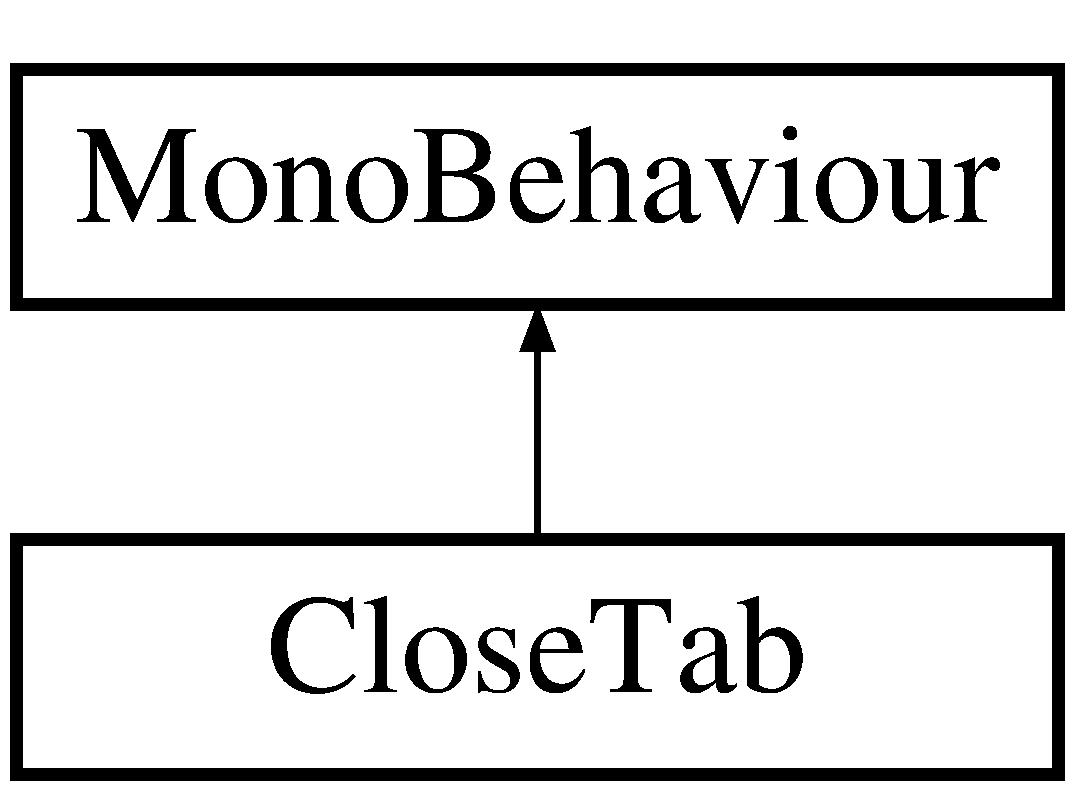
\includegraphics[height=2.000000cm]{class_close_tab}
\end{center}
\end{figure}
\subsection*{Public Attributes}
\begin{DoxyCompactItemize}
\item 
\mbox{\Hypertarget{class_close_tab_a99ebb029c1a1b54330d23663f4475ec1}\label{class_close_tab_a99ebb029c1a1b54330d23663f4475ec1}} 
Button {\bfseries your\+Button}
\item 
\mbox{\Hypertarget{class_close_tab_a24b8d522b292a5c726753d11973a7044}\label{class_close_tab_a24b8d522b292a5c726753d11973a7044}} 
Game\+Object {\bfseries parent}
\item 
\mbox{\Hypertarget{class_close_tab_af479316a53d722614c1b31d0a9857ef7}\label{class_close_tab_af479316a53d722614c1b31d0a9857ef7}} 
\hyperlink{class_model_controller}{Model\+Controller} {\bfseries mc}
\end{DoxyCompactItemize}


\subsection{Detailed Description}
Button that closes its tab when clicked 



The documentation for this class was generated from the following file\+:\begin{DoxyCompactItemize}
\item 
Close\+Tab.\+cs\end{DoxyCompactItemize}

\hypertarget{class_console_script}{}\section{Console\+Script Class Reference}
\label{class_console_script}\index{Console\+Script@{Console\+Script}}


W\+IP Debugging console of the tool  


Inheritance diagram for Console\+Script\+:\begin{figure}[H]
\begin{center}
\leavevmode
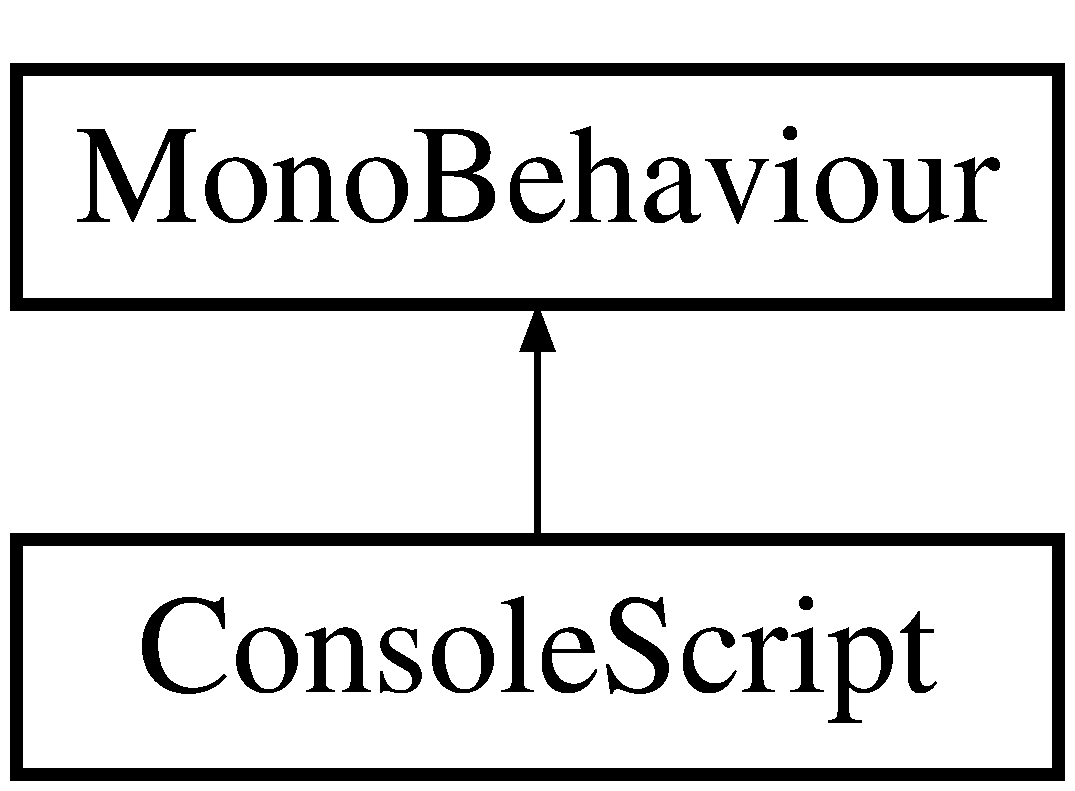
\includegraphics[height=2.000000cm]{class_console_script}
\end{center}
\end{figure}
\subsection*{Public Member Functions}
\begin{DoxyCompactItemize}
\item 
void \hyperlink{class_console_script_a1c1670e872384c1bc97b8bbeecbb0e08}{Display\+Error} (Error\+Type type, string text, Game\+Object tab, List$<$ Game\+Object $>$ objects)
\begin{DoxyCompactList}\small\item\em Displays the error message in the console \end{DoxyCompactList}\item 
\mbox{\Hypertarget{class_console_script_a4adcec6051afdbbeaa152d4d9a5fdb35}\label{class_console_script_a4adcec6051afdbbeaa152d4d9a5fdb35}} 
void {\bfseries Go\+To\+Error} ()
\end{DoxyCompactItemize}
\subsection*{Public Attributes}
\begin{DoxyCompactItemize}
\item 
\mbox{\Hypertarget{class_console_script_a354d1061b55468819d14a4d709b5a759}\label{class_console_script_a354d1061b55468819d14a4d709b5a759}} 
Text {\bfseries console\+Text}
\item 
\mbox{\Hypertarget{class_console_script_addd68fdcc48b4929f1c5f71ed4880fb5}\label{class_console_script_addd68fdcc48b4929f1c5f71ed4880fb5}} 
Button {\bfseries console\+Button}
\item 
\mbox{\Hypertarget{class_console_script_ade9e2262d3a3159072b69a4548b1a02e}\label{class_console_script_ade9e2262d3a3159072b69a4548b1a02e}} 
Game\+Object {\bfseries error\+Tab}
\end{DoxyCompactItemize}


\subsection{Detailed Description}
W\+IP Debugging console of the tool 



\subsection{Member Function Documentation}
\mbox{\Hypertarget{class_console_script_a1c1670e872384c1bc97b8bbeecbb0e08}\label{class_console_script_a1c1670e872384c1bc97b8bbeecbb0e08}} 
\index{Console\+Script@{Console\+Script}!Display\+Error@{Display\+Error}}
\index{Display\+Error@{Display\+Error}!Console\+Script@{Console\+Script}}
\subsubsection{\texorpdfstring{Display\+Error()}{DisplayError()}}
{\footnotesize\ttfamily void Console\+Script.\+Display\+Error (\begin{DoxyParamCaption}\item[{Error\+Type}]{type,  }\item[{string}]{text,  }\item[{Game\+Object}]{tab,  }\item[{List$<$ Game\+Object $>$}]{objects }\end{DoxyParamCaption})}



Displays the error message in the console 


\begin{DoxyParams}{Parameters}
{\em type} & Type of the error\\
\hline
{\em text} & The error message\\
\hline
{\em tab} & Source of the error (definition)\\
\hline
{\em objects} & \\
\hline
\end{DoxyParams}


The documentation for this class was generated from the following file\+:\begin{DoxyCompactItemize}
\item 
Console\+Script.\+cs\end{DoxyCompactItemize}

\hypertarget{class_definition_script}{}\section{Definition\+Script Class Reference}
\label{class_definition_script}\index{Definition\+Script@{Definition\+Script}}


This script controls the locations of interface nodes on a definition T\+O\+DO\+: Rethink the placement of interface nodes/make them interactable  


Inheritance diagram for Definition\+Script\+:\begin{figure}[H]
\begin{center}
\leavevmode
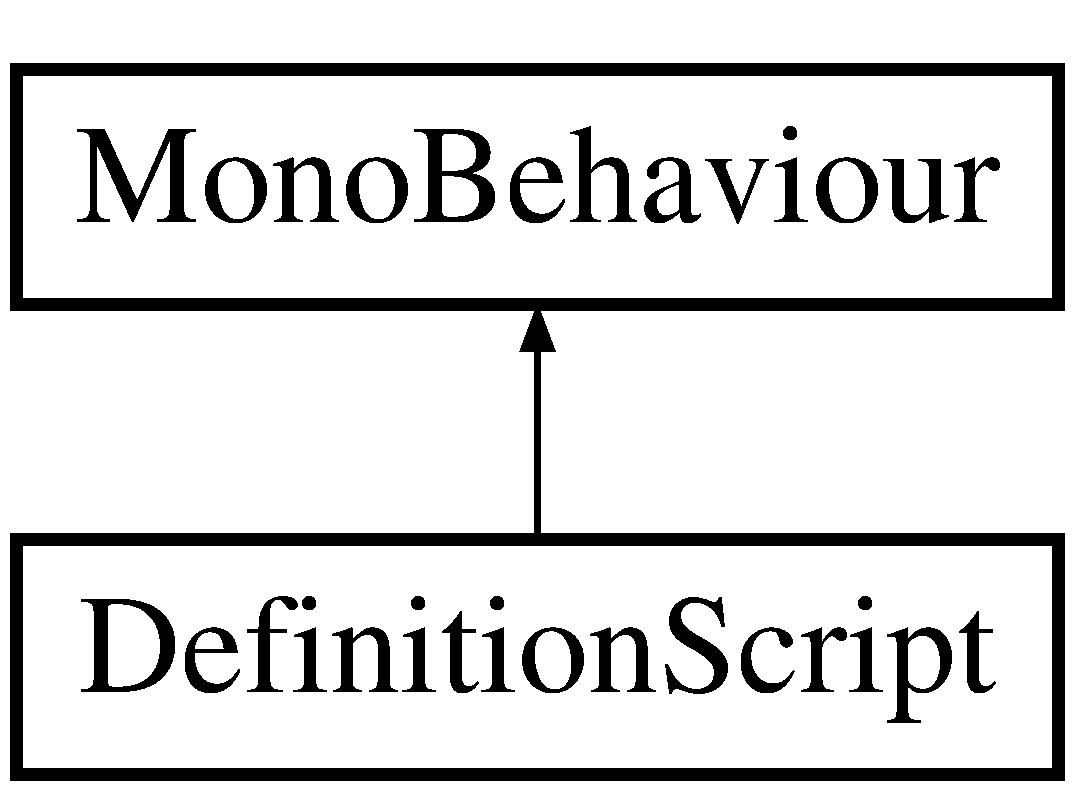
\includegraphics[height=2.000000cm]{class_definition_script}
\end{center}
\end{figure}
\subsection*{Public Member Functions}
\begin{DoxyCompactItemize}
\item 
void \hyperlink{class_definition_script_aa024bbcd14da56aba2a845998453d1ae}{Add\+Reference\+Point} (Game\+Object newref)
\begin{DoxyCompactList}\small\item\em Adds a reference point to the definition \end{DoxyCompactList}\item 
void \hyperlink{class_definition_script_a1e2cd233f3dff31d405c2a5dcd2bad37}{Remove\+Reference\+Point} (Game\+Object removed\+Ref)
\begin{DoxyCompactList}\small\item\em Removes a reference point from the definition \end{DoxyCompactList}\item 
void \hyperlink{class_definition_script_a8cb4f36965c85361ae6cb466596e2afd}{Clear\+Reference\+Points} ()
\begin{DoxyCompactList}\small\item\em Removes all reference points \end{DoxyCompactList}\end{DoxyCompactItemize}
\subsection*{Public Attributes}
\begin{DoxyCompactItemize}
\item 
\mbox{\Hypertarget{class_definition_script_ad47da0ed9e66100c5a3a8e647cbef7b4}\label{class_definition_script_ad47da0ed9e66100c5a3a8e647cbef7b4}} 
Game\+Object {\bfseries reference\+Point}
\item 
\mbox{\Hypertarget{class_definition_script_ade8635fab94307e175a20c484fb5dbfc}\label{class_definition_script_ade8635fab94307e175a20c484fb5dbfc}} 
List$<$ Game\+Object $>$ {\bfseries references}
\item 
\mbox{\Hypertarget{class_definition_script_a9d97e6bf584887710cf839fe855443d0}\label{class_definition_script_a9d97e6bf584887710cf839fe855443d0}} 
List$<$ Game\+Object $>$ {\bfseries reference\+Points}
\end{DoxyCompactItemize}


\subsection{Detailed Description}
This script controls the locations of interface nodes on a definition T\+O\+DO\+: Rethink the placement of interface nodes/make them interactable 



\subsection{Member Function Documentation}
\mbox{\Hypertarget{class_definition_script_aa024bbcd14da56aba2a845998453d1ae}\label{class_definition_script_aa024bbcd14da56aba2a845998453d1ae}} 
\index{Definition\+Script@{Definition\+Script}!Add\+Reference\+Point@{Add\+Reference\+Point}}
\index{Add\+Reference\+Point@{Add\+Reference\+Point}!Definition\+Script@{Definition\+Script}}
\subsubsection{\texorpdfstring{Add\+Reference\+Point()}{AddReferencePoint()}}
{\footnotesize\ttfamily void Definition\+Script.\+Add\+Reference\+Point (\begin{DoxyParamCaption}\item[{Game\+Object}]{newref }\end{DoxyParamCaption})}



Adds a reference point to the definition 


\begin{DoxyParams}{Parameters}
{\em newref} & The reference point to be added\\
\hline
\end{DoxyParams}
\mbox{\Hypertarget{class_definition_script_a8cb4f36965c85361ae6cb466596e2afd}\label{class_definition_script_a8cb4f36965c85361ae6cb466596e2afd}} 
\index{Definition\+Script@{Definition\+Script}!Clear\+Reference\+Points@{Clear\+Reference\+Points}}
\index{Clear\+Reference\+Points@{Clear\+Reference\+Points}!Definition\+Script@{Definition\+Script}}
\subsubsection{\texorpdfstring{Clear\+Reference\+Points()}{ClearReferencePoints()}}
{\footnotesize\ttfamily void Definition\+Script.\+Clear\+Reference\+Points (\begin{DoxyParamCaption}{ }\end{DoxyParamCaption})}



Removes all reference points 

\mbox{\Hypertarget{class_definition_script_a1e2cd233f3dff31d405c2a5dcd2bad37}\label{class_definition_script_a1e2cd233f3dff31d405c2a5dcd2bad37}} 
\index{Definition\+Script@{Definition\+Script}!Remove\+Reference\+Point@{Remove\+Reference\+Point}}
\index{Remove\+Reference\+Point@{Remove\+Reference\+Point}!Definition\+Script@{Definition\+Script}}
\subsubsection{\texorpdfstring{Remove\+Reference\+Point()}{RemoveReferencePoint()}}
{\footnotesize\ttfamily void Definition\+Script.\+Remove\+Reference\+Point (\begin{DoxyParamCaption}\item[{Game\+Object}]{removed\+Ref }\end{DoxyParamCaption})}



Removes a reference point from the definition 


\begin{DoxyParams}{Parameters}
{\em removed\+Ref} & The reference point to be removed\\
\hline
\end{DoxyParams}


The documentation for this class was generated from the following file\+:\begin{DoxyCompactItemize}
\item 
Definition\+Script.\+cs\end{DoxyCompactItemize}

\hypertarget{class_dynamic_tab}{}\section{Dynamic\+Tab Class Reference}
\label{class_dynamic_tab}\index{Dynamic\+Tab@{Dynamic\+Tab}}


This script moves and scales the tabs when needed  


Inheritance diagram for Dynamic\+Tab\+:\begin{figure}[H]
\begin{center}
\leavevmode
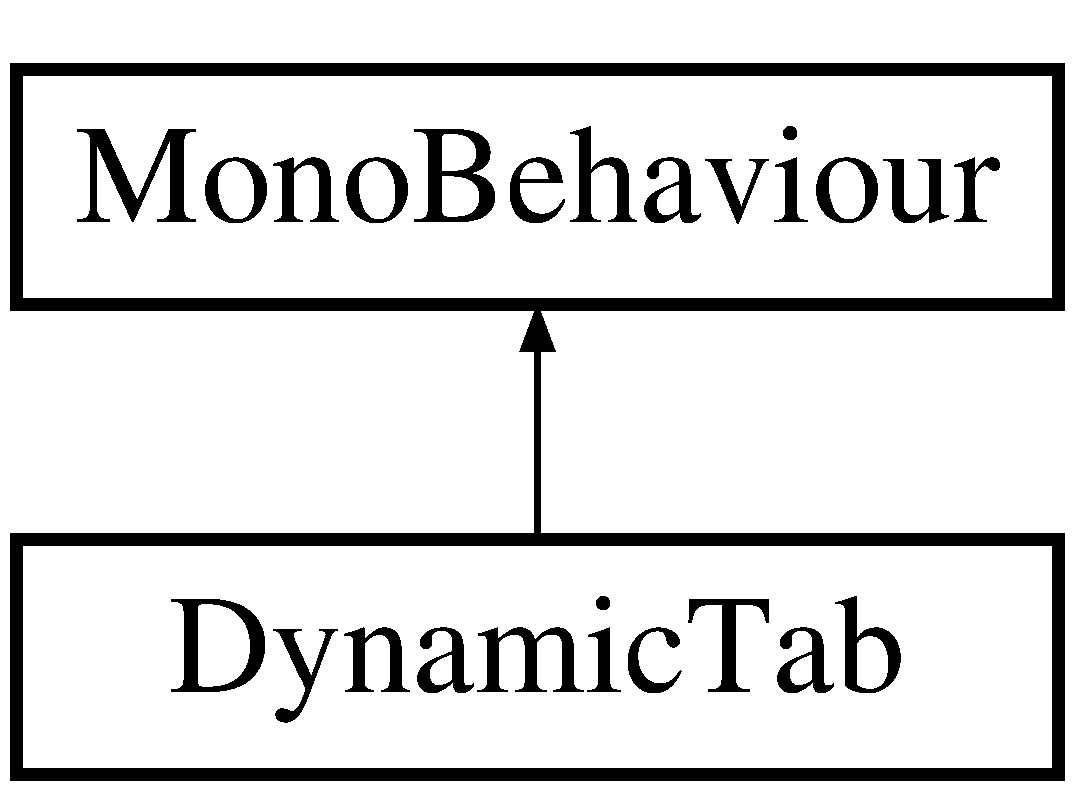
\includegraphics[height=2.000000cm]{class_dynamic_tab}
\end{center}
\end{figure}
\subsection*{Public Member Functions}
\begin{DoxyCompactItemize}
\item 
void \hyperlink{class_dynamic_tab_a6aadee2864c08657e3e87eac95f6174a}{Move\+Up} ()
\begin{DoxyCompactList}\small\item\em Moves the tab up (scales with scale variable) \end{DoxyCompactList}\item 
void \hyperlink{class_dynamic_tab_a95fcdcd13d54ad12dfcd46375fd85647}{Move\+Down} ()
\begin{DoxyCompactList}\small\item\em Moves the tab down if it\textquotesingle{}s not the leftmost tab (scales with scale variable) \end{DoxyCompactList}\item 
void \hyperlink{class_dynamic_tab_acedc824d9b337ce9877170c90974ae89}{Scale\+Down} ()
\begin{DoxyCompactList}\small\item\em Decreases the scale and corrects position according to new width. \end{DoxyCompactList}\item 
void \hyperlink{class_dynamic_tab_ab215a9f1108a089155cef53d9a529661}{Scale\+Up} ()
\begin{DoxyCompactList}\small\item\em Increases scale and corrects position according to new width. \end{DoxyCompactList}\item 
void \hyperlink{class_dynamic_tab_a17b150a9b2c6d126ae719a1f20da9272}{On\+Click} ()
\begin{DoxyCompactList}\small\item\em When clicked the tab notifies other objects that a tab has been selected \end{DoxyCompactList}\end{DoxyCompactItemize}
\subsection*{Public Attributes}
\begin{DoxyCompactItemize}
\item 
\mbox{\Hypertarget{class_dynamic_tab_a3310820127321a8259f84b78ac0b663d}\label{class_dynamic_tab_a3310820127321a8259f84b78ac0b663d}} 
int {\bfseries tab\+Index}
\item 
\mbox{\Hypertarget{class_dynamic_tab_a52b9c75b4b0d66f44f8e87d9bb3198a2}\label{class_dynamic_tab_a52b9c75b4b0d66f44f8e87d9bb3198a2}} 
Game\+Object \mbox{[}$\,$\mbox{]} {\bfseries tabs}
\item 
\mbox{\Hypertarget{class_dynamic_tab_a8cba12f6445bab7de712f1f5b9a8a468}\label{class_dynamic_tab_a8cba12f6445bab7de712f1f5b9a8a468}} 
float {\bfseries scale} = 1.\+0f
\item 
\mbox{\Hypertarget{class_dynamic_tab_a5696016eddfb72ac561885e07a3280a9}\label{class_dynamic_tab_a5696016eddfb72ac561885e07a3280a9}} 
Button {\bfseries your\+Button}
\item 
\mbox{\Hypertarget{class_dynamic_tab_ab198a7ba270fd8dfa47c2d1b09bf6ed7}\label{class_dynamic_tab_ab198a7ba270fd8dfa47c2d1b09bf6ed7}} 
Rect\+Transform {\bfseries grid\+Tab}
\end{DoxyCompactItemize}


\subsection{Detailed Description}
This script moves and scales the tabs when needed 



\subsection{Member Function Documentation}
\mbox{\Hypertarget{class_dynamic_tab_a95fcdcd13d54ad12dfcd46375fd85647}\label{class_dynamic_tab_a95fcdcd13d54ad12dfcd46375fd85647}} 
\index{Dynamic\+Tab@{Dynamic\+Tab}!Move\+Down@{Move\+Down}}
\index{Move\+Down@{Move\+Down}!Dynamic\+Tab@{Dynamic\+Tab}}
\subsubsection{\texorpdfstring{Move\+Down()}{MoveDown()}}
{\footnotesize\ttfamily void Dynamic\+Tab.\+Move\+Down (\begin{DoxyParamCaption}{ }\end{DoxyParamCaption})}



Moves the tab down if it\textquotesingle{}s not the leftmost tab (scales with scale variable) 

\mbox{\Hypertarget{class_dynamic_tab_a6aadee2864c08657e3e87eac95f6174a}\label{class_dynamic_tab_a6aadee2864c08657e3e87eac95f6174a}} 
\index{Dynamic\+Tab@{Dynamic\+Tab}!Move\+Up@{Move\+Up}}
\index{Move\+Up@{Move\+Up}!Dynamic\+Tab@{Dynamic\+Tab}}
\subsubsection{\texorpdfstring{Move\+Up()}{MoveUp()}}
{\footnotesize\ttfamily void Dynamic\+Tab.\+Move\+Up (\begin{DoxyParamCaption}{ }\end{DoxyParamCaption})}



Moves the tab up (scales with scale variable) 

\mbox{\Hypertarget{class_dynamic_tab_a17b150a9b2c6d126ae719a1f20da9272}\label{class_dynamic_tab_a17b150a9b2c6d126ae719a1f20da9272}} 
\index{Dynamic\+Tab@{Dynamic\+Tab}!On\+Click@{On\+Click}}
\index{On\+Click@{On\+Click}!Dynamic\+Tab@{Dynamic\+Tab}}
\subsubsection{\texorpdfstring{On\+Click()}{OnClick()}}
{\footnotesize\ttfamily void Dynamic\+Tab.\+On\+Click (\begin{DoxyParamCaption}{ }\end{DoxyParamCaption})}



When clicked the tab notifies other objects that a tab has been selected 

\mbox{\Hypertarget{class_dynamic_tab_acedc824d9b337ce9877170c90974ae89}\label{class_dynamic_tab_acedc824d9b337ce9877170c90974ae89}} 
\index{Dynamic\+Tab@{Dynamic\+Tab}!Scale\+Down@{Scale\+Down}}
\index{Scale\+Down@{Scale\+Down}!Dynamic\+Tab@{Dynamic\+Tab}}
\subsubsection{\texorpdfstring{Scale\+Down()}{ScaleDown()}}
{\footnotesize\ttfamily void Dynamic\+Tab.\+Scale\+Down (\begin{DoxyParamCaption}{ }\end{DoxyParamCaption})}



Decreases the scale and corrects position according to new width. 

\mbox{\Hypertarget{class_dynamic_tab_ab215a9f1108a089155cef53d9a529661}\label{class_dynamic_tab_ab215a9f1108a089155cef53d9a529661}} 
\index{Dynamic\+Tab@{Dynamic\+Tab}!Scale\+Up@{Scale\+Up}}
\index{Scale\+Up@{Scale\+Up}!Dynamic\+Tab@{Dynamic\+Tab}}
\subsubsection{\texorpdfstring{Scale\+Up()}{ScaleUp()}}
{\footnotesize\ttfamily void Dynamic\+Tab.\+Scale\+Up (\begin{DoxyParamCaption}{ }\end{DoxyParamCaption})}



Increases scale and corrects position according to new width. 



The documentation for this class was generated from the following file\+:\begin{DoxyCompactItemize}
\item 
Dynamic\+Tab.\+cs\end{DoxyCompactItemize}

\hypertarget{class_edge_inspector}{}\section{Edge\+Inspector Class Reference}
\label{class_edge_inspector}\index{Edge\+Inspector@{Edge\+Inspector}}


The edge inspector  


Inheritance diagram for Edge\+Inspector\+:\begin{figure}[H]
\begin{center}
\leavevmode
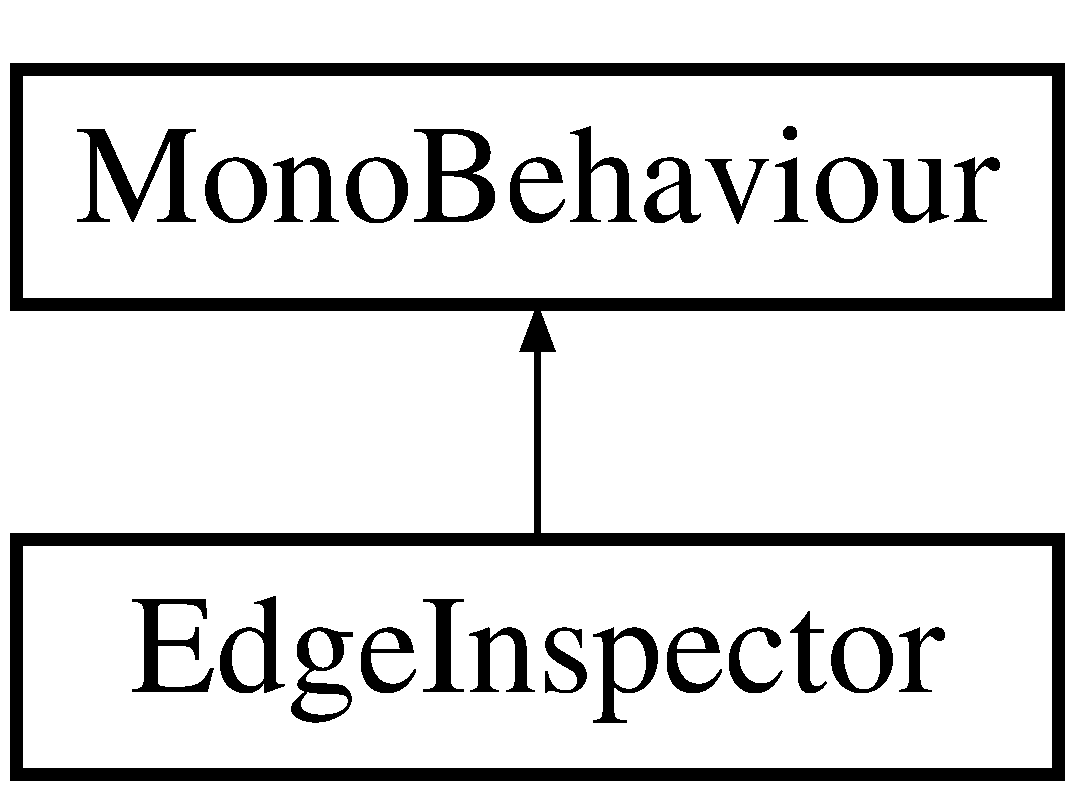
\includegraphics[height=2.000000cm]{class_edge_inspector}
\end{center}
\end{figure}
\subsection*{Public Member Functions}
\begin{DoxyCompactItemize}
\item 
void \hyperlink{class_edge_inspector_a92090d3f3e51f3f0c164c457d3be8eea}{Select} (Game\+Object selected\+Object)
\begin{DoxyCompactList}\small\item\em Selects given object in the edge inspector \end{DoxyCompactList}\item 
void \hyperlink{class_edge_inspector_a695897e9dfd53c8d147f2897d3ff21f9}{Deselect} ()
\begin{DoxyCompactList}\small\item\em Clears selection of the Edge Inspector. \end{DoxyCompactList}\item 
void \hyperlink{class_edge_inspector_a156a07db25d54510f00a336943474fcc}{Update\+Name} ()
\begin{DoxyCompactList}\small\item\em Updates the Name of the currently selected node. \end{DoxyCompactList}\item 
void \hyperlink{class_edge_inspector_a513fd82ff3e791570874421df36ddd9f}{Update\+Source} ()
\begin{DoxyCompactList}\small\item\em Updates the Behavior component of the currently selected node. \end{DoxyCompactList}\item 
void \hyperlink{class_edge_inspector_a2516d546da9c4b3c74f29608a712fa27}{Update\+Exp} ()
\begin{DoxyCompactList}\small\item\em Updates the At component of the currently selected node. \end{DoxyCompactList}\item 
void \hyperlink{class_edge_inspector_a6e6050bef0c14197e73f848ebcab7ecf}{Update\+Target} ()
\begin{DoxyCompactList}\small\item\em Updates the Max component of the currently selected node. \end{DoxyCompactList}\end{DoxyCompactItemize}
\subsection*{Public Attributes}
\begin{DoxyCompactItemize}
\item 
\mbox{\Hypertarget{class_edge_inspector_aef5538a8549c97fd20dc29883515fef6}\label{class_edge_inspector_aef5538a8549c97fd20dc29883515fef6}} 
Transform {\bfseries canvas}
\item 
\mbox{\Hypertarget{class_edge_inspector_ab8ddb57092c75c120e99bd7c14235f92}\label{class_edge_inspector_ab8ddb57092c75c120e99bd7c14235f92}} 
Game\+Object {\bfseries content}
\item 
\mbox{\Hypertarget{class_edge_inspector_a9ddd0f1774c0255e2a28c62dab834dc7}\label{class_edge_inspector_a9ddd0f1774c0255e2a28c62dab834dc7}} 
\hyperlink{class_model_controller}{Model\+Controller} {\bfseries mc}
\item 
\mbox{\Hypertarget{class_edge_inspector_a407d4896703cf2b1ad9df82215401cb1}\label{class_edge_inspector_a407d4896703cf2b1ad9df82215401cb1}} 
Game\+Object {\bfseries selected\+Edge}
\item 
\mbox{\Hypertarget{class_edge_inspector_a3c05353b79341451a68e4371a073d135}\label{class_edge_inspector_a3c05353b79341451a68e4371a073d135}} 
Input\+Field {\bfseries label}
\item 
\mbox{\Hypertarget{class_edge_inspector_a1682bdf6df01a5f678bb724ffb570178}\label{class_edge_inspector_a1682bdf6df01a5f678bb724ffb570178}} 
Input\+Field {\bfseries source}
\item 
\mbox{\Hypertarget{class_edge_inspector_ae5ad1583e1de5f55731dc23f7873f371}\label{class_edge_inspector_ae5ad1583e1de5f55731dc23f7873f371}} 
Input\+Field {\bfseries exp}
\item 
\mbox{\Hypertarget{class_edge_inspector_ae3cc5d7ce122499fd60573b0290c66d1}\label{class_edge_inspector_ae3cc5d7ce122499fd60573b0290c66d1}} 
Input\+Field {\bfseries target}
\item 
\mbox{\Hypertarget{class_edge_inspector_af8e567cee5b567dcdbdfc7b2f96fe84d}\label{class_edge_inspector_af8e567cee5b567dcdbdfc7b2f96fe84d}} 
Dropdown {\bfseries typedd}
\item 
\mbox{\Hypertarget{class_edge_inspector_a6a8258041c8542711dd7f08b4ba9ee95}\label{class_edge_inspector_a6a8258041c8542711dd7f08b4ba9ee95}} 
string {\bfseries active\+Tab\+Name}
\end{DoxyCompactItemize}


\subsection{Detailed Description}
The edge inspector 



\subsection{Member Function Documentation}
\mbox{\Hypertarget{class_edge_inspector_a695897e9dfd53c8d147f2897d3ff21f9}\label{class_edge_inspector_a695897e9dfd53c8d147f2897d3ff21f9}} 
\index{Edge\+Inspector@{Edge\+Inspector}!Deselect@{Deselect}}
\index{Deselect@{Deselect}!Edge\+Inspector@{Edge\+Inspector}}
\subsubsection{\texorpdfstring{Deselect()}{Deselect()}}
{\footnotesize\ttfamily void Edge\+Inspector.\+Deselect (\begin{DoxyParamCaption}{ }\end{DoxyParamCaption})}



Clears selection of the Edge Inspector. 

\mbox{\Hypertarget{class_edge_inspector_a92090d3f3e51f3f0c164c457d3be8eea}\label{class_edge_inspector_a92090d3f3e51f3f0c164c457d3be8eea}} 
\index{Edge\+Inspector@{Edge\+Inspector}!Select@{Select}}
\index{Select@{Select}!Edge\+Inspector@{Edge\+Inspector}}
\subsubsection{\texorpdfstring{Select()}{Select()}}
{\footnotesize\ttfamily void Edge\+Inspector.\+Select (\begin{DoxyParamCaption}\item[{Game\+Object}]{selected\+Object }\end{DoxyParamCaption})}



Selects given object in the edge inspector 


\begin{DoxyParams}{Parameters}
{\em selected\+Object} & the object that needs to be inspected \\
\hline
\end{DoxyParams}
\mbox{\Hypertarget{class_edge_inspector_a2516d546da9c4b3c74f29608a712fa27}\label{class_edge_inspector_a2516d546da9c4b3c74f29608a712fa27}} 
\index{Edge\+Inspector@{Edge\+Inspector}!Update\+Exp@{Update\+Exp}}
\index{Update\+Exp@{Update\+Exp}!Edge\+Inspector@{Edge\+Inspector}}
\subsubsection{\texorpdfstring{Update\+Exp()}{UpdateExp()}}
{\footnotesize\ttfamily void Edge\+Inspector.\+Update\+Exp (\begin{DoxyParamCaption}{ }\end{DoxyParamCaption})}



Updates the At component of the currently selected node. 

\mbox{\Hypertarget{class_edge_inspector_a156a07db25d54510f00a336943474fcc}\label{class_edge_inspector_a156a07db25d54510f00a336943474fcc}} 
\index{Edge\+Inspector@{Edge\+Inspector}!Update\+Name@{Update\+Name}}
\index{Update\+Name@{Update\+Name}!Edge\+Inspector@{Edge\+Inspector}}
\subsubsection{\texorpdfstring{Update\+Name()}{UpdateName()}}
{\footnotesize\ttfamily void Edge\+Inspector.\+Update\+Name (\begin{DoxyParamCaption}{ }\end{DoxyParamCaption})}



Updates the Name of the currently selected node. 

\mbox{\Hypertarget{class_edge_inspector_a513fd82ff3e791570874421df36ddd9f}\label{class_edge_inspector_a513fd82ff3e791570874421df36ddd9f}} 
\index{Edge\+Inspector@{Edge\+Inspector}!Update\+Source@{Update\+Source}}
\index{Update\+Source@{Update\+Source}!Edge\+Inspector@{Edge\+Inspector}}
\subsubsection{\texorpdfstring{Update\+Source()}{UpdateSource()}}
{\footnotesize\ttfamily void Edge\+Inspector.\+Update\+Source (\begin{DoxyParamCaption}{ }\end{DoxyParamCaption})}



Updates the Behavior component of the currently selected node. 

\mbox{\Hypertarget{class_edge_inspector_a6e6050bef0c14197e73f848ebcab7ecf}\label{class_edge_inspector_a6e6050bef0c14197e73f848ebcab7ecf}} 
\index{Edge\+Inspector@{Edge\+Inspector}!Update\+Target@{Update\+Target}}
\index{Update\+Target@{Update\+Target}!Edge\+Inspector@{Edge\+Inspector}}
\subsubsection{\texorpdfstring{Update\+Target()}{UpdateTarget()}}
{\footnotesize\ttfamily void Edge\+Inspector.\+Update\+Target (\begin{DoxyParamCaption}{ }\end{DoxyParamCaption})}



Updates the Max component of the currently selected node. 



The documentation for this class was generated from the following file\+:\begin{DoxyCompactItemize}
\item 
Edge\+Inspector.\+cs\end{DoxyCompactItemize}

\hypertarget{class_editor_button_script}{}\section{Editor\+Button\+Script Class Reference}
\label{class_editor_button_script}\index{Editor\+Button\+Script@{Editor\+Button\+Script}}


Button script for the tool selection buttons in the editor  


Inheritance diagram for Editor\+Button\+Script\+:\begin{figure}[H]
\begin{center}
\leavevmode
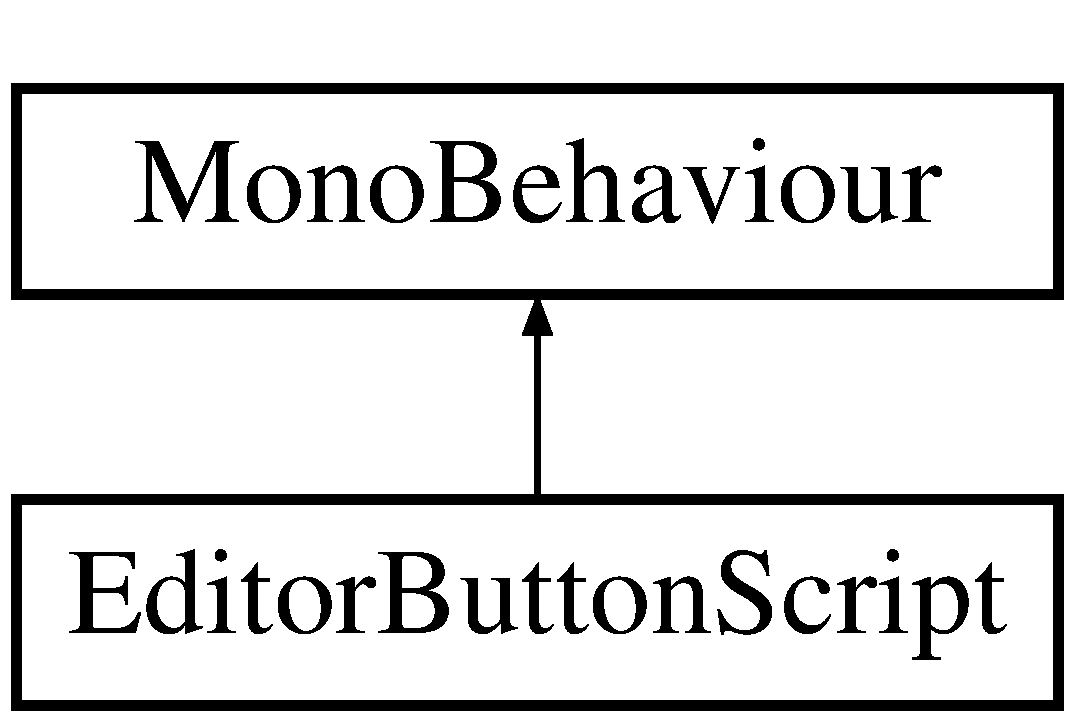
\includegraphics[height=2.000000cm]{class_editor_button_script}
\end{center}
\end{figure}
\subsection*{Public Attributes}
\begin{DoxyCompactItemize}
\item 
\mbox{\Hypertarget{class_editor_button_script_ac1393bbefbbc3b763f4dfd842005439e}\label{class_editor_button_script_ac1393bbefbbc3b763f4dfd842005439e}} 
Button {\bfseries your\+Button}
\item 
Behavior \hyperlink{class_editor_button_script_a7df9834d8c560512d210be3c1454edd9}{type}
\begin{DoxyCompactList}\small\item\em This enum is used as the type of tool the \hyperlink{class_model_view_controller}{Model\+View\+Controller} is using \end{DoxyCompactList}\item 
\mbox{\Hypertarget{class_editor_button_script_ab0b733ec12c57bf5c1a1a199ddae92c9}\label{class_editor_button_script_ab0b733ec12c57bf5c1a1a199ddae92c9}} 
Transform {\bfseries canvas}
\item 
\mbox{\Hypertarget{class_editor_button_script_afc2d0a5f774c41306ed7cafb4b71273f}\label{class_editor_button_script_afc2d0a5f774c41306ed7cafb4b71273f}} 
Transform {\bfseries current\+Grid}
\end{DoxyCompactItemize}


\subsection{Detailed Description}
Button script for the tool selection buttons in the editor 



\subsection{Member Data Documentation}
\mbox{\Hypertarget{class_editor_button_script_a7df9834d8c560512d210be3c1454edd9}\label{class_editor_button_script_a7df9834d8c560512d210be3c1454edd9}} 
\index{Editor\+Button\+Script@{Editor\+Button\+Script}!type@{type}}
\index{type@{type}!Editor\+Button\+Script@{Editor\+Button\+Script}}
\subsubsection{\texorpdfstring{type}{type}}
{\footnotesize\ttfamily Behavior Editor\+Button\+Script.\+type}



This enum is used as the type of tool the \hyperlink{class_model_view_controller}{Model\+View\+Controller} is using 



The documentation for this class was generated from the following file\+:\begin{DoxyCompactItemize}
\item 
Editor\+Button\+Script.\+cs\end{DoxyCompactItemize}

\hypertarget{class_event_manager}{}\section{Event\+Manager Class Reference}
\label{class_event_manager}\index{Event\+Manager@{Event\+Manager}}


Standard Event Manager  


Inheritance diagram for Event\+Manager\+:\begin{figure}[H]
\begin{center}
\leavevmode
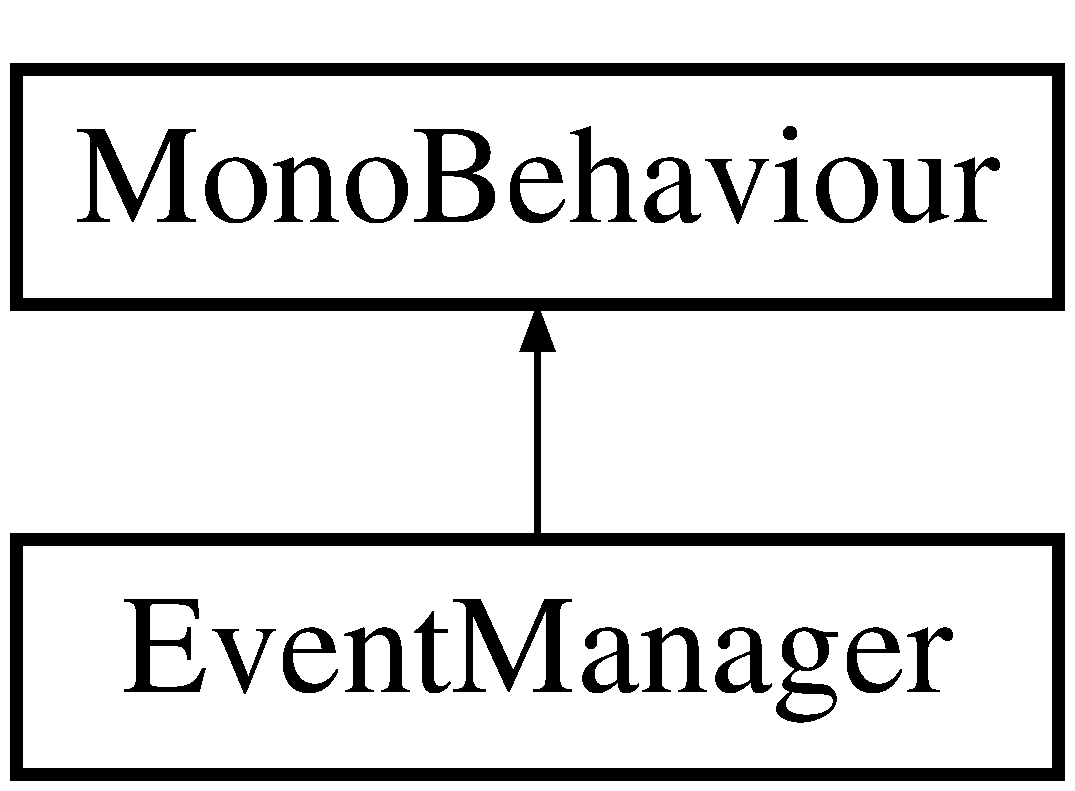
\includegraphics[height=2.000000cm]{class_event_manager}
\end{center}
\end{figure}
\subsection*{Static Public Member Functions}
\begin{DoxyCompactItemize}
\item 
\mbox{\Hypertarget{class_event_manager_a0bbc4d6c0420fd5c4cd108da486ec3f5}\label{class_event_manager_a0bbc4d6c0420fd5c4cd108da486ec3f5}} 
static void {\bfseries Start\+Listening} (string event\+Name, Unity\+Action listener)
\item 
\mbox{\Hypertarget{class_event_manager_a4dd92dc8fc89cfec873035c852de9d29}\label{class_event_manager_a4dd92dc8fc89cfec873035c852de9d29}} 
static void {\bfseries Stop\+Listening} (string event\+Name, Unity\+Action listener)
\item 
\mbox{\Hypertarget{class_event_manager_a41b32d95b222220546f131806504c8ac}\label{class_event_manager_a41b32d95b222220546f131806504c8ac}} 
static void {\bfseries Trigger\+Event} (string event\+Name)
\end{DoxyCompactItemize}
\subsection*{Static Public Attributes}
\begin{DoxyCompactItemize}
\item 
\mbox{\Hypertarget{class_event_manager_a8d0d8ab42da1ba97f200f912f76e2c52}\label{class_event_manager_a8d0d8ab42da1ba97f200f912f76e2c52}} 
static \hyperlink{class_event_manager}{Event\+Manager} {\bfseries event\+Manager}
\end{DoxyCompactItemize}
\subsection*{Properties}
\begin{DoxyCompactItemize}
\item 
\mbox{\Hypertarget{class_event_manager_a48dc961602569f67255381442e7bbd2d}\label{class_event_manager_a48dc961602569f67255381442e7bbd2d}} 
static \hyperlink{class_event_manager}{Event\+Manager} {\bfseries instance}\hspace{0.3cm}{\ttfamily  \mbox{[}get\mbox{]}}
\end{DoxyCompactItemize}


\subsection{Detailed Description}
Standard Event Manager 



The documentation for this class was generated from the following file\+:\begin{DoxyCompactItemize}
\item 
Event\+Manager.\+cs\end{DoxyCompactItemize}

\hypertarget{class_exit_button}{}\section{Exit\+Button Class Reference}
\label{class_exit_button}\index{Exit\+Button@{Exit\+Button}}


Button that closes the tool  


Inheritance diagram for Exit\+Button\+:\begin{figure}[H]
\begin{center}
\leavevmode
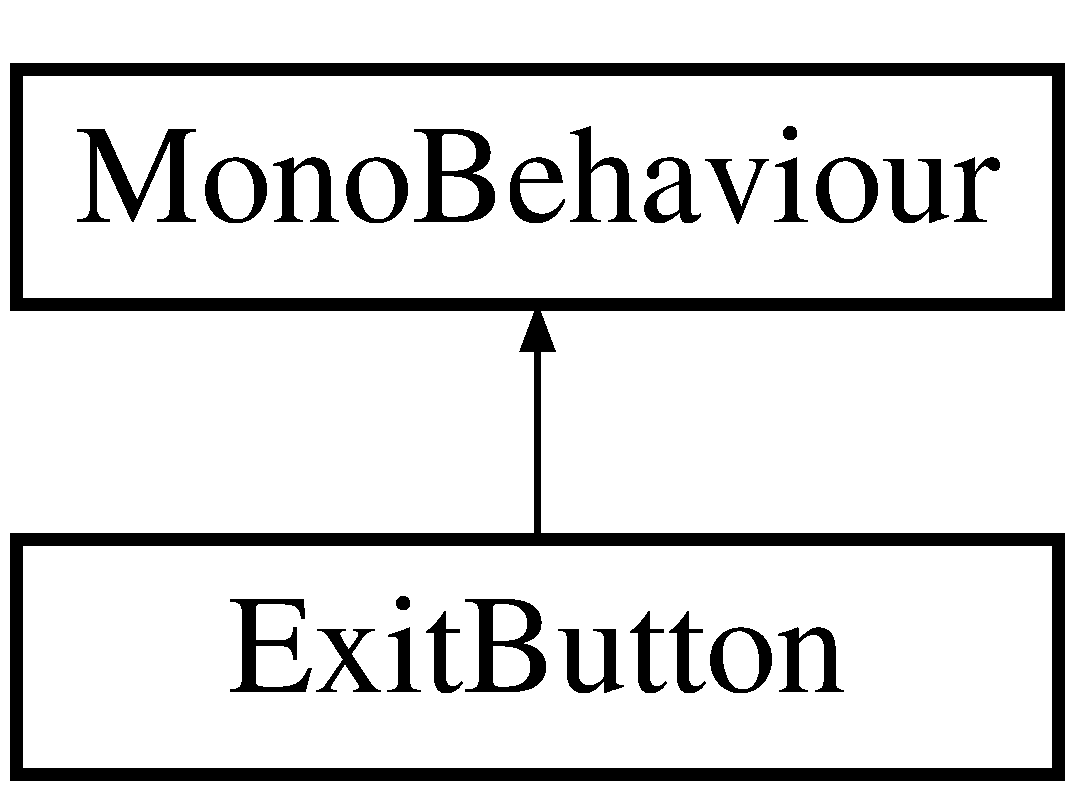
\includegraphics[height=2.000000cm]{class_exit_button}
\end{center}
\end{figure}
\subsection*{Public Member Functions}
\begin{DoxyCompactItemize}
\item 
\mbox{\Hypertarget{class_exit_button_a689f0ce74a0fa78627bacac651fe25e0}\label{class_exit_button_a689f0ce74a0fa78627bacac651fe25e0}} 
delegate void {\bfseries exit} ()
\end{DoxyCompactItemize}
\subsection*{Public Attributes}
\begin{DoxyCompactItemize}
\item 
\mbox{\Hypertarget{class_exit_button_ad1a0ea5a36ad96f8d614eead8a744e7d}\label{class_exit_button_ad1a0ea5a36ad96f8d614eead8a744e7d}} 
Button {\bfseries your\+Button}
\end{DoxyCompactItemize}
\subsection*{Events}
\begin{DoxyCompactItemize}
\item 
\mbox{\Hypertarget{class_exit_button_abbded8cc172dc6f50de83891fb5d8a14}\label{class_exit_button_abbded8cc172dc6f50de83891fb5d8a14}} 
static exit {\bfseries On\+Exit}
\end{DoxyCompactItemize}


\subsection{Detailed Description}
Button that closes the tool 



The documentation for this class was generated from the following file\+:\begin{DoxyCompactItemize}
\item 
Exit\+Button.\+cs\end{DoxyCompactItemize}

\hypertarget{class_export_file_script}{}\section{Export\+File\+Script Class Reference}
\label{class_export_file_script}\index{Export\+File\+Script@{Export\+File\+Script}}
Inheritance diagram for Export\+File\+Script\+:\begin{figure}[H]
\begin{center}
\leavevmode
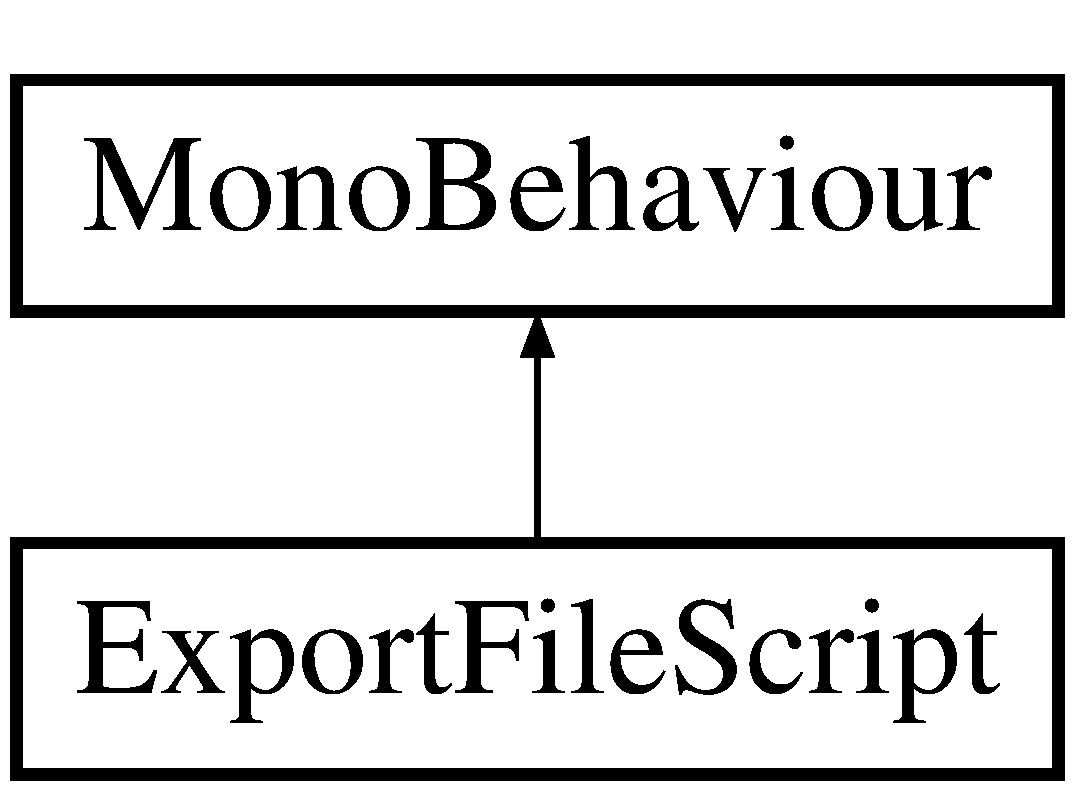
\includegraphics[height=2.000000cm]{class_export_file_script}
\end{center}
\end{figure}
\subsection*{Public Attributes}
\begin{DoxyCompactItemize}
\item 
\mbox{\Hypertarget{class_export_file_script_a2e4ef21d66a1ce7ee1a3c578f85b6ff8}\label{class_export_file_script_a2e4ef21d66a1ce7ee1a3c578f85b6ff8}} 
Unity\+Engine.\+U\+I.\+Button {\bfseries your\+Button}
\item 
\mbox{\Hypertarget{class_export_file_script_a364eb6176f7876754539dd3812b3fa08}\label{class_export_file_script_a364eb6176f7876754539dd3812b3fa08}} 
string {\bfseries path} = null
\item 
\mbox{\Hypertarget{class_export_file_script_a22da1b1ddd76aa4e037c1200ee678bda}\label{class_export_file_script_a22da1b1ddd76aa4e037c1200ee678bda}} 
\hyperlink{class_model_controller}{Model\+Controller} {\bfseries mc}
\end{DoxyCompactItemize}


The documentation for this class was generated from the following file\+:\begin{DoxyCompactItemize}
\item 
Export\+File\+Script.\+cs\end{DoxyCompactItemize}

\hypertarget{class_model_controller}{}\section{Model\+Controller Class Reference}
\label{class_model_controller}\index{Model\+Controller@{Model\+Controller}}


Communication between Visual model and technical Micro-\/\+Machinations model.  


Inheritance diagram for Model\+Controller\+:\begin{figure}[H]
\begin{center}
\leavevmode
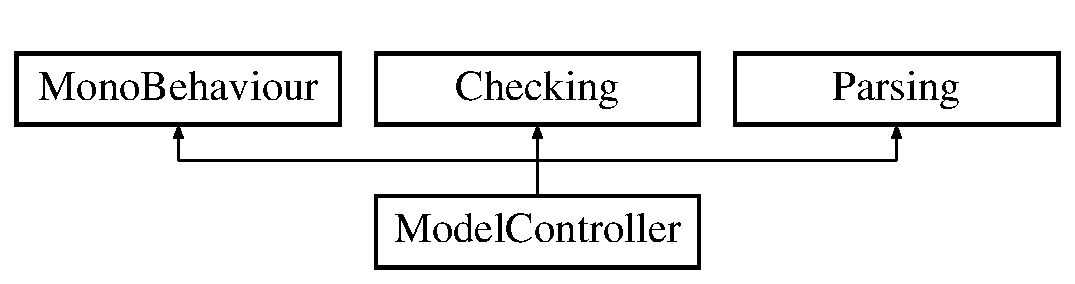
\includegraphics[height=2.000000cm]{class_model_controller}
\end{center}
\end{figure}
\subsection*{Public Member Functions}
\begin{DoxyCompactItemize}
\item 
void \hyperlink{class_model_controller_ace07b89fa66aa3855d9fd888e98d3c07}{receive} (M\+M.\+Parser.\+Parser\+Message message)
\begin{DoxyCompactList}\small\item\em Receives error/warning messages from the parser T\+O\+DO\+: Use the tools own console instead of unity debugger. \end{DoxyCompactList}\item 
void \hyperlink{class_model_controller_ad66a01d17f0bdff7f3a668e8dd37fd43}{receive} (M\+M.\+Runtime.\+Checker\+Message message)
\begin{DoxyCompactList}\small\item\em Receives error/warning messages from the runtime model T\+O\+DO\+: Use the tools own console instead of unity debugger. \end{DoxyCompactList}\item 
\mbox{\Hypertarget{class_model_controller_aeb277810748a80f9a3b9478d92c91b7b}\label{class_model_controller_aeb277810748a80f9a3b9478d92c91b7b}} 
void {\bfseries Start} ()
\item 
void \hyperlink{class_model_controller_add55c5cac76924f59e57adffee93ae79}{Add\+Edge} (Behavior edgebehavior, string def\+Name, Game\+Object newedgeobj)
\begin{DoxyCompactList}\small\item\em Adds an edge to the model \end{DoxyCompactList}\item 
void \hyperlink{class_model_controller_a19cbb949bcd04111795784724d883975}{Add\+Node} (Behavior added\+Node\+Type, Vector2 new\+Node\+Pos, string def\+Name, Game\+Object newnodeobj)
\begin{DoxyCompactList}\small\item\em Adds a node to the model \end{DoxyCompactList}\item 
void \hyperlink{class_model_controller_a7bdefba3d9a2445710046462819bb5dd}{Update\+Node\+Max} (int newmax, string tabname, M\+M.\+Model.\+Node updated\+Node)
\begin{DoxyCompactList}\small\item\em Updates the max variable of a specific node \end{DoxyCompactList}\item 
void \hyperlink{class_model_controller_a0e667937f2c81e87b6fa8a501aea09b9}{Update\+Node\+Add} (string newadd, M\+M.\+Model.\+Node updated\+Node, string tabname)
\begin{DoxyCompactList}\small\item\em Updates the add variable of a specific node \end{DoxyCompactList}\item 
void \hyperlink{class_model_controller_a98a3ea019f3d366a0f91d3536f96a1c3}{Update\+Node\+Definition} (string newdefname, M\+M.\+Model.\+Node newnodeobj, string tabname)
\begin{DoxyCompactList}\small\item\em Updates the typeof variable of a specific node \end{DoxyCompactList}\item 
void \hyperlink{class_model_controller_ae9cfb758e08532565a361a02cdad420f}{Update\+Node\+How} (How newhow, M\+M.\+Model.\+Node newnodeobj, string tabname)
\begin{DoxyCompactList}\small\item\em Updates the how variable of a specific node \end{DoxyCompactList}\item 
void \hyperlink{class_model_controller_add94ec175f5f81a3acb57a33f958c3a5}{Update\+Node\+Act} (Act newact, M\+M.\+Model.\+Node newnodeobj, string tabname)
\begin{DoxyCompactList}\small\item\em Updates the act variable of a specific node \end{DoxyCompactList}\item 
void \hyperlink{class_model_controller_a008c60f8bb31f6525f116b7b9cd7107b}{Update\+Node\+When} (When newwhen, M\+M.\+Model.\+Node newnodeobj, string tabname)
\begin{DoxyCompactList}\small\item\em Updates the when variable of a specific node \end{DoxyCompactList}\item 
void \hyperlink{class_model_controller_aefda67a5dfdc0b8dd5dfc8811d42a52a}{Update\+Node\+IO} (IO newio, M\+M.\+Model.\+Node newnodeobj, string tabname)
\begin{DoxyCompactList}\small\item\em Updates the io variable of a specific node \end{DoxyCompactList}\item 
void \hyperlink{class_model_controller_acd6773a9b3bd6bacec227104838d5403}{Update\+Node\+At} (int newat, M\+M.\+Model.\+Node newnodeobj, string tabname)
\begin{DoxyCompactList}\small\item\em Updates the at variable of a specific node \end{DoxyCompactList}\item 
void \hyperlink{class_model_controller_a2bc7d852f482d7190094602734029097}{Update\+Node\+Name} (string newname, M\+M.\+Model.\+Node newnodeobj, string tabname)
\begin{DoxyCompactList}\small\item\em Updates the name of a specific node \end{DoxyCompactList}\item 
void \hyperlink{class_model_controller_a5b2ce36e6894c3e41f42b4f9dc0d9b06}{Update\+Node\+Behavior} (Behavior newtype, M\+M.\+Model.\+Node newnodeobj, string tabname)
\begin{DoxyCompactList}\small\item\em Updates the behavior of a specific node \end{DoxyCompactList}\item 
void \hyperlink{class_model_controller_a184dc2424e87afbec8dc12e99f2f2451}{Update\+Node\+Position} (Vector2 new\+Pos, string tabname, M\+M.\+Model.\+Node newnodeobj)
\begin{DoxyCompactList}\small\item\em Updates the position of a specific node \end{DoxyCompactList}\item 
void \hyperlink{class_model_controller_ae55705c9c541f326757e2a4ba0310af0}{Update\+Edge\+Name} (string newname, M\+M.\+Model.\+Edge newedgeobj, string tabname)
\begin{DoxyCompactList}\small\item\em Updates the name of a specific edge \end{DoxyCompactList}\item 
void \hyperlink{class_model_controller_aaa7910a28a9feb7e6086cec6aba33613}{Update\+Edge\+Source} (string newsourcename, M\+M.\+Model.\+Edge newedgeobj, string tabname)
\begin{DoxyCompactList}\small\item\em Updates the source of a specific edge \end{DoxyCompactList}\item 
void \hyperlink{class_model_controller_afc082aa500c60243108b67e509d62ef2}{Update\+Edge\+Target} (string newtargetname, M\+M.\+Model.\+Edge newedgeobj, string tabname)
\begin{DoxyCompactList}\small\item\em Updates the target of a specific edge \end{DoxyCompactList}\item 
void \hyperlink{class_model_controller_a06912800fa56c444b0a54a2e777460a0}{Update\+Edge\+Expression} (string newexpression, M\+M.\+Model.\+Edge newedgeobj, string tabname)
\begin{DoxyCompactList}\small\item\em Updates the expression of a specific edge \end{DoxyCompactList}\item 
void \hyperlink{class_model_controller_a366347bcb88a5d9741341cb42d9617b6}{Add\+Program} ()
\begin{DoxyCompactList}\small\item\em Creates the program in the machine \end{DoxyCompactList}\item 
void \hyperlink{class_model_controller_ae0ed52e43c07b4f6ed37488d5e3bd5e0}{Add\+Definition} (string name)
\begin{DoxyCompactList}\small\item\em Checks if there is a program (if not calls Add\+Program) then adds a definition to it. \end{DoxyCompactList}\item 
void \hyperlink{class_model_controller_ad8870c7c6be199c58b77cb4f3f666bea}{Update\+Definition} (string old\+Name, string new\+Name)
\begin{DoxyCompactList}\small\item\em Updates the name of a definition \end{DoxyCompactList}\item 
void \hyperlink{class_model_controller_a6a33ac19aff3ce293c7c2e4255e50470}{Delete\+Definition} (string defname)
\begin{DoxyCompactList}\small\item\em Removes the target definition from the model \end{DoxyCompactList}\item 
void \hyperlink{class_model_controller_ad9f66266f49a332182e57d2368801e5f}{Delete\+Node} (M\+M.\+Model.\+Node removednode, string tabname)
\begin{DoxyCompactList}\small\item\em Removes the target node from the model \end{DoxyCompactList}\item 
void \hyperlink{class_model_controller_af810eecc43d27f5790958b9900ff1215}{Delete\+Flow\+Edge} (M\+M.\+Model.\+Flow\+Edge removededge, string tabname)
\begin{DoxyCompactList}\small\item\em Removes the target flow edge from the model \end{DoxyCompactList}\item 
void \hyperlink{class_model_controller_aa941845548865a4f06a78537f78ec236}{Delete\+State\+Edge} (M\+M.\+Model.\+State\+Edge removededge, string tabname)
\begin{DoxyCompactList}\small\item\em Removes the target state edge from the model \end{DoxyCompactList}\item 
void \hyperlink{class_model_controller_a992f56918cbedc3e57c22d5365eee9cb}{Set\+Program} (M\+M.\+Model.\+Program p)
\begin{DoxyCompactList}\small\item\em Set local program to p \end{DoxyCompactList}\item 
void \hyperlink{class_model_controller_a9ccde31addae7d655b85fb38872aa3ea}{Set\+Machine} (M\+M.\+Machine m)
\begin{DoxyCompactList}\small\item\em Set local machine to m \end{DoxyCompactList}\item 
void \hyperlink{class_model_controller_a961f8ecc991434e6751ddc1f63864509}{Export\+To\+File} (string filepath)
\begin{DoxyCompactList}\small\item\em Print model to text file \end{DoxyCompactList}\end{DoxyCompactItemize}
\subsection*{Public Attributes}
\begin{DoxyCompactItemize}
\item 
\mbox{\Hypertarget{class_model_controller_af756f6d794d6ed6e8a5537eeb36a4d35}\label{class_model_controller_af756f6d794d6ed6e8a5537eeb36a4d35}} 
M\+M.\+Model.\+Program {\bfseries prog} = null
\item 
\mbox{\Hypertarget{class_model_controller_aba32734969a12343eb585ca8256bbcd9}\label{class_model_controller_aba32734969a12343eb585ca8256bbcd9}} 
M\+M.\+Machine {\bfseries machine}
\end{DoxyCompactItemize}


\subsection{Detailed Description}
Communication between Visual model and technical Micro-\/\+Machinations model. 



\subsection{Member Function Documentation}
\mbox{\Hypertarget{class_model_controller_ae0ed52e43c07b4f6ed37488d5e3bd5e0}\label{class_model_controller_ae0ed52e43c07b4f6ed37488d5e3bd5e0}} 
\index{Model\+Controller@{Model\+Controller}!Add\+Definition@{Add\+Definition}}
\index{Add\+Definition@{Add\+Definition}!Model\+Controller@{Model\+Controller}}
\subsubsection{\texorpdfstring{Add\+Definition()}{AddDefinition()}}
{\footnotesize\ttfamily void Model\+Controller.\+Add\+Definition (\begin{DoxyParamCaption}\item[{string}]{name }\end{DoxyParamCaption})}



Checks if there is a program (if not calls Add\+Program) then adds a definition to it. 


\begin{DoxyParams}{Parameters}
{\em name} & \\
\hline
\end{DoxyParams}
\mbox{\Hypertarget{class_model_controller_add55c5cac76924f59e57adffee93ae79}\label{class_model_controller_add55c5cac76924f59e57adffee93ae79}} 
\index{Model\+Controller@{Model\+Controller}!Add\+Edge@{Add\+Edge}}
\index{Add\+Edge@{Add\+Edge}!Model\+Controller@{Model\+Controller}}
\subsubsection{\texorpdfstring{Add\+Edge()}{AddEdge()}}
{\footnotesize\ttfamily void Model\+Controller.\+Add\+Edge (\begin{DoxyParamCaption}\item[{Behavior}]{edgebehavior,  }\item[{string}]{def\+Name,  }\item[{Game\+Object}]{newedgeobj }\end{DoxyParamCaption})}



Adds an edge to the model 


\begin{DoxyParams}{Parameters}
{\em edgebehavior} & The type of edge added (Flow or State)\\
\hline
{\em def\+Name} & Name of the definition this edge was added to\\
\hline
{\em newedgeobj} & The unity object of the added edge\\
\hline
\end{DoxyParams}
\mbox{\Hypertarget{class_model_controller_a19cbb949bcd04111795784724d883975}\label{class_model_controller_a19cbb949bcd04111795784724d883975}} 
\index{Model\+Controller@{Model\+Controller}!Add\+Node@{Add\+Node}}
\index{Add\+Node@{Add\+Node}!Model\+Controller@{Model\+Controller}}
\subsubsection{\texorpdfstring{Add\+Node()}{AddNode()}}
{\footnotesize\ttfamily void Model\+Controller.\+Add\+Node (\begin{DoxyParamCaption}\item[{Behavior}]{added\+Node\+Type,  }\item[{Vector2}]{new\+Node\+Pos,  }\item[{string}]{def\+Name,  }\item[{Game\+Object}]{newnodeobj }\end{DoxyParamCaption})}



Adds a node to the model 


\begin{DoxyParams}{Parameters}
{\em added\+Node\+Type} & Behavior of the new node (Pool, Source, Drain etc.)\\
\hline
{\em new\+Node\+Pos} & Position of the new node on screen\\
\hline
{\em def\+Name} & Name of the definition this node was added to\\
\hline
{\em newnodeobj} & The unity object of the added node\\
\hline
\end{DoxyParams}
\mbox{\Hypertarget{class_model_controller_a366347bcb88a5d9741341cb42d9617b6}\label{class_model_controller_a366347bcb88a5d9741341cb42d9617b6}} 
\index{Model\+Controller@{Model\+Controller}!Add\+Program@{Add\+Program}}
\index{Add\+Program@{Add\+Program}!Model\+Controller@{Model\+Controller}}
\subsubsection{\texorpdfstring{Add\+Program()}{AddProgram()}}
{\footnotesize\ttfamily void Model\+Controller.\+Add\+Program (\begin{DoxyParamCaption}{ }\end{DoxyParamCaption})}



Creates the program in the machine 

\mbox{\Hypertarget{class_model_controller_a6a33ac19aff3ce293c7c2e4255e50470}\label{class_model_controller_a6a33ac19aff3ce293c7c2e4255e50470}} 
\index{Model\+Controller@{Model\+Controller}!Delete\+Definition@{Delete\+Definition}}
\index{Delete\+Definition@{Delete\+Definition}!Model\+Controller@{Model\+Controller}}
\subsubsection{\texorpdfstring{Delete\+Definition()}{DeleteDefinition()}}
{\footnotesize\ttfamily void Model\+Controller.\+Delete\+Definition (\begin{DoxyParamCaption}\item[{string}]{defname }\end{DoxyParamCaption})}



Removes the target definition from the model 


\begin{DoxyParams}{Parameters}
{\em defname} & Definition name that needs to be removed\\
\hline
\end{DoxyParams}
\mbox{\Hypertarget{class_model_controller_af810eecc43d27f5790958b9900ff1215}\label{class_model_controller_af810eecc43d27f5790958b9900ff1215}} 
\index{Model\+Controller@{Model\+Controller}!Delete\+Flow\+Edge@{Delete\+Flow\+Edge}}
\index{Delete\+Flow\+Edge@{Delete\+Flow\+Edge}!Model\+Controller@{Model\+Controller}}
\subsubsection{\texorpdfstring{Delete\+Flow\+Edge()}{DeleteFlowEdge()}}
{\footnotesize\ttfamily void Model\+Controller.\+Delete\+Flow\+Edge (\begin{DoxyParamCaption}\item[{M\+M.\+Model.\+Flow\+Edge}]{removededge,  }\item[{string}]{tabname }\end{DoxyParamCaption})}



Removes the target flow edge from the model 


\begin{DoxyParams}{Parameters}
{\em removededge} & Flow edge object that needs to be removed\\
\hline
{\em tabname} & Definition name containing the target edge\\
\hline
\end{DoxyParams}
\mbox{\Hypertarget{class_model_controller_ad9f66266f49a332182e57d2368801e5f}\label{class_model_controller_ad9f66266f49a332182e57d2368801e5f}} 
\index{Model\+Controller@{Model\+Controller}!Delete\+Node@{Delete\+Node}}
\index{Delete\+Node@{Delete\+Node}!Model\+Controller@{Model\+Controller}}
\subsubsection{\texorpdfstring{Delete\+Node()}{DeleteNode()}}
{\footnotesize\ttfamily void Model\+Controller.\+Delete\+Node (\begin{DoxyParamCaption}\item[{M\+M.\+Model.\+Node}]{removednode,  }\item[{string}]{tabname }\end{DoxyParamCaption})}



Removes the target node from the model 


\begin{DoxyParams}{Parameters}
{\em removednode} & Node object that needs to be removed\\
\hline
{\em tabname} & Definition name containing the target node\\
\hline
\end{DoxyParams}
\mbox{\Hypertarget{class_model_controller_aa941845548865a4f06a78537f78ec236}\label{class_model_controller_aa941845548865a4f06a78537f78ec236}} 
\index{Model\+Controller@{Model\+Controller}!Delete\+State\+Edge@{Delete\+State\+Edge}}
\index{Delete\+State\+Edge@{Delete\+State\+Edge}!Model\+Controller@{Model\+Controller}}
\subsubsection{\texorpdfstring{Delete\+State\+Edge()}{DeleteStateEdge()}}
{\footnotesize\ttfamily void Model\+Controller.\+Delete\+State\+Edge (\begin{DoxyParamCaption}\item[{M\+M.\+Model.\+State\+Edge}]{removededge,  }\item[{string}]{tabname }\end{DoxyParamCaption})}



Removes the target state edge from the model 


\begin{DoxyParams}{Parameters}
{\em removededge} & State edge object that needs to be removed\\
\hline
{\em tabname} & Definition name containing the target edge\\
\hline
\end{DoxyParams}
\mbox{\Hypertarget{class_model_controller_a961f8ecc991434e6751ddc1f63864509}\label{class_model_controller_a961f8ecc991434e6751ddc1f63864509}} 
\index{Model\+Controller@{Model\+Controller}!Export\+To\+File@{Export\+To\+File}}
\index{Export\+To\+File@{Export\+To\+File}!Model\+Controller@{Model\+Controller}}
\subsubsection{\texorpdfstring{Export\+To\+File()}{ExportToFile()}}
{\footnotesize\ttfamily void Model\+Controller.\+Export\+To\+File (\begin{DoxyParamCaption}\item[{string}]{filepath }\end{DoxyParamCaption})}



Print model to text file 


\begin{DoxyParams}{Parameters}
{\em filepath} & File path for text file\\
\hline
\end{DoxyParams}
\mbox{\Hypertarget{class_model_controller_ace07b89fa66aa3855d9fd888e98d3c07}\label{class_model_controller_ace07b89fa66aa3855d9fd888e98d3c07}} 
\index{Model\+Controller@{Model\+Controller}!receive@{receive}}
\index{receive@{receive}!Model\+Controller@{Model\+Controller}}
\subsubsection{\texorpdfstring{receive()}{receive()}\hspace{0.1cm}{\footnotesize\ttfamily [1/2]}}
{\footnotesize\ttfamily void Model\+Controller.\+receive (\begin{DoxyParamCaption}\item[{M\+M.\+Parser.\+Parser\+Message}]{message }\end{DoxyParamCaption})}



Receives error/warning messages from the parser T\+O\+DO\+: Use the tools own console instead of unity debugger. 


\begin{DoxyParams}{Parameters}
{\em message} & The error message received\\
\hline
\end{DoxyParams}
\mbox{\Hypertarget{class_model_controller_ad66a01d17f0bdff7f3a668e8dd37fd43}\label{class_model_controller_ad66a01d17f0bdff7f3a668e8dd37fd43}} 
\index{Model\+Controller@{Model\+Controller}!receive@{receive}}
\index{receive@{receive}!Model\+Controller@{Model\+Controller}}
\subsubsection{\texorpdfstring{receive()}{receive()}\hspace{0.1cm}{\footnotesize\ttfamily [2/2]}}
{\footnotesize\ttfamily void Model\+Controller.\+receive (\begin{DoxyParamCaption}\item[{M\+M.\+Runtime.\+Checker\+Message}]{message }\end{DoxyParamCaption})}



Receives error/warning messages from the runtime model T\+O\+DO\+: Use the tools own console instead of unity debugger. 


\begin{DoxyParams}{Parameters}
{\em message} & The error message received\\
\hline
\end{DoxyParams}
\mbox{\Hypertarget{class_model_controller_a9ccde31addae7d655b85fb38872aa3ea}\label{class_model_controller_a9ccde31addae7d655b85fb38872aa3ea}} 
\index{Model\+Controller@{Model\+Controller}!Set\+Machine@{Set\+Machine}}
\index{Set\+Machine@{Set\+Machine}!Model\+Controller@{Model\+Controller}}
\subsubsection{\texorpdfstring{Set\+Machine()}{SetMachine()}}
{\footnotesize\ttfamily void Model\+Controller.\+Set\+Machine (\begin{DoxyParamCaption}\item[{M\+M.\+Machine}]{m }\end{DoxyParamCaption})}



Set local machine to m 


\begin{DoxyParams}{Parameters}
{\em m} & Micro-\/\+Machinations machine\\
\hline
\end{DoxyParams}
\mbox{\Hypertarget{class_model_controller_a992f56918cbedc3e57c22d5365eee9cb}\label{class_model_controller_a992f56918cbedc3e57c22d5365eee9cb}} 
\index{Model\+Controller@{Model\+Controller}!Set\+Program@{Set\+Program}}
\index{Set\+Program@{Set\+Program}!Model\+Controller@{Model\+Controller}}
\subsubsection{\texorpdfstring{Set\+Program()}{SetProgram()}}
{\footnotesize\ttfamily void Model\+Controller.\+Set\+Program (\begin{DoxyParamCaption}\item[{M\+M.\+Model.\+Program}]{p }\end{DoxyParamCaption})}



Set local program to p 


\begin{DoxyParams}{Parameters}
{\em p} & Micro-\/\+Machinations model program \\
\hline
\end{DoxyParams}
\mbox{\Hypertarget{class_model_controller_ad8870c7c6be199c58b77cb4f3f666bea}\label{class_model_controller_ad8870c7c6be199c58b77cb4f3f666bea}} 
\index{Model\+Controller@{Model\+Controller}!Update\+Definition@{Update\+Definition}}
\index{Update\+Definition@{Update\+Definition}!Model\+Controller@{Model\+Controller}}
\subsubsection{\texorpdfstring{Update\+Definition()}{UpdateDefinition()}}
{\footnotesize\ttfamily void Model\+Controller.\+Update\+Definition (\begin{DoxyParamCaption}\item[{string}]{old\+Name,  }\item[{string}]{new\+Name }\end{DoxyParamCaption})}



Updates the name of a definition 


\begin{DoxyParams}{Parameters}
{\em old\+Name} & Old name of the definition used to identify it\\
\hline
{\em new\+Name} & New name of the definition\\
\hline
\end{DoxyParams}
\mbox{\Hypertarget{class_model_controller_a06912800fa56c444b0a54a2e777460a0}\label{class_model_controller_a06912800fa56c444b0a54a2e777460a0}} 
\index{Model\+Controller@{Model\+Controller}!Update\+Edge\+Expression@{Update\+Edge\+Expression}}
\index{Update\+Edge\+Expression@{Update\+Edge\+Expression}!Model\+Controller@{Model\+Controller}}
\subsubsection{\texorpdfstring{Update\+Edge\+Expression()}{UpdateEdgeExpression()}}
{\footnotesize\ttfamily void Model\+Controller.\+Update\+Edge\+Expression (\begin{DoxyParamCaption}\item[{string}]{newexpression,  }\item[{M\+M.\+Model.\+Edge}]{newedgeobj,  }\item[{string}]{tabname }\end{DoxyParamCaption})}



Updates the expression of a specific edge 


\begin{DoxyParams}{Parameters}
{\em newexpression} & New expression\\
\hline
{\em newedgeobj} & The edge model object that needs to be changed\\
\hline
{\em tabname} & Name of the definition the changed edge is in\\
\hline
\end{DoxyParams}
\mbox{\Hypertarget{class_model_controller_ae55705c9c541f326757e2a4ba0310af0}\label{class_model_controller_ae55705c9c541f326757e2a4ba0310af0}} 
\index{Model\+Controller@{Model\+Controller}!Update\+Edge\+Name@{Update\+Edge\+Name}}
\index{Update\+Edge\+Name@{Update\+Edge\+Name}!Model\+Controller@{Model\+Controller}}
\subsubsection{\texorpdfstring{Update\+Edge\+Name()}{UpdateEdgeName()}}
{\footnotesize\ttfamily void Model\+Controller.\+Update\+Edge\+Name (\begin{DoxyParamCaption}\item[{string}]{newname,  }\item[{M\+M.\+Model.\+Edge}]{newedgeobj,  }\item[{string}]{tabname }\end{DoxyParamCaption})}



Updates the name of a specific edge 


\begin{DoxyParams}{Parameters}
{\em newname} & New name\\
\hline
{\em newedgeobj} & The edge model object that needs to be changed\\
\hline
{\em tabname} & Name of the definition the changed edge is in\\
\hline
\end{DoxyParams}
\mbox{\Hypertarget{class_model_controller_aaa7910a28a9feb7e6086cec6aba33613}\label{class_model_controller_aaa7910a28a9feb7e6086cec6aba33613}} 
\index{Model\+Controller@{Model\+Controller}!Update\+Edge\+Source@{Update\+Edge\+Source}}
\index{Update\+Edge\+Source@{Update\+Edge\+Source}!Model\+Controller@{Model\+Controller}}
\subsubsection{\texorpdfstring{Update\+Edge\+Source()}{UpdateEdgeSource()}}
{\footnotesize\ttfamily void Model\+Controller.\+Update\+Edge\+Source (\begin{DoxyParamCaption}\item[{string}]{newsourcename,  }\item[{M\+M.\+Model.\+Edge}]{newedgeobj,  }\item[{string}]{tabname }\end{DoxyParamCaption})}



Updates the source of a specific edge 


\begin{DoxyParams}{Parameters}
{\em newsourcename} & Name of the new source\\
\hline
{\em newedgeobj} & The edge model object that needs to be changed\\
\hline
{\em tabname} & Name of the definition the changed edge is in\\
\hline
\end{DoxyParams}
\mbox{\Hypertarget{class_model_controller_afc082aa500c60243108b67e509d62ef2}\label{class_model_controller_afc082aa500c60243108b67e509d62ef2}} 
\index{Model\+Controller@{Model\+Controller}!Update\+Edge\+Target@{Update\+Edge\+Target}}
\index{Update\+Edge\+Target@{Update\+Edge\+Target}!Model\+Controller@{Model\+Controller}}
\subsubsection{\texorpdfstring{Update\+Edge\+Target()}{UpdateEdgeTarget()}}
{\footnotesize\ttfamily void Model\+Controller.\+Update\+Edge\+Target (\begin{DoxyParamCaption}\item[{string}]{newtargetname,  }\item[{M\+M.\+Model.\+Edge}]{newedgeobj,  }\item[{string}]{tabname }\end{DoxyParamCaption})}



Updates the target of a specific edge 


\begin{DoxyParams}{Parameters}
{\em newtargetname} & Name of the new target\\
\hline
{\em newedgeobj} & The edge model object that needs to be changed\\
\hline
{\em tabname} & Name of the definition the changed edge is in\\
\hline
\end{DoxyParams}
\mbox{\Hypertarget{class_model_controller_add94ec175f5f81a3acb57a33f958c3a5}\label{class_model_controller_add94ec175f5f81a3acb57a33f958c3a5}} 
\index{Model\+Controller@{Model\+Controller}!Update\+Node\+Act@{Update\+Node\+Act}}
\index{Update\+Node\+Act@{Update\+Node\+Act}!Model\+Controller@{Model\+Controller}}
\subsubsection{\texorpdfstring{Update\+Node\+Act()}{UpdateNodeAct()}}
{\footnotesize\ttfamily void Model\+Controller.\+Update\+Node\+Act (\begin{DoxyParamCaption}\item[{Act}]{newact,  }\item[{M\+M.\+Model.\+Node}]{newnodeobj,  }\item[{string}]{tabname }\end{DoxyParamCaption})}



Updates the act variable of a specific node 


\begin{DoxyParams}{Parameters}
{\em newact} & New value for act\\
\hline
{\em newnodeobj} & The node model object that needs to be changed\\
\hline
{\em tabname} & Name of the definition the changed node is in\\
\hline
\end{DoxyParams}
\mbox{\Hypertarget{class_model_controller_a0e667937f2c81e87b6fa8a501aea09b9}\label{class_model_controller_a0e667937f2c81e87b6fa8a501aea09b9}} 
\index{Model\+Controller@{Model\+Controller}!Update\+Node\+Add@{Update\+Node\+Add}}
\index{Update\+Node\+Add@{Update\+Node\+Add}!Model\+Controller@{Model\+Controller}}
\subsubsection{\texorpdfstring{Update\+Node\+Add()}{UpdateNodeAdd()}}
{\footnotesize\ttfamily void Model\+Controller.\+Update\+Node\+Add (\begin{DoxyParamCaption}\item[{string}]{newadd,  }\item[{M\+M.\+Model.\+Node}]{updated\+Node,  }\item[{string}]{tabname }\end{DoxyParamCaption})}



Updates the add variable of a specific node 


\begin{DoxyParams}{Parameters}
{\em newadd} & New value for add\\
\hline
{\em updated\+Node} & The node model object that needs to be changed\\
\hline
{\em tabname} & Name of the definition the changed node is in\\
\hline
\end{DoxyParams}
\mbox{\Hypertarget{class_model_controller_acd6773a9b3bd6bacec227104838d5403}\label{class_model_controller_acd6773a9b3bd6bacec227104838d5403}} 
\index{Model\+Controller@{Model\+Controller}!Update\+Node\+At@{Update\+Node\+At}}
\index{Update\+Node\+At@{Update\+Node\+At}!Model\+Controller@{Model\+Controller}}
\subsubsection{\texorpdfstring{Update\+Node\+At()}{UpdateNodeAt()}}
{\footnotesize\ttfamily void Model\+Controller.\+Update\+Node\+At (\begin{DoxyParamCaption}\item[{int}]{newat,  }\item[{M\+M.\+Model.\+Node}]{newnodeobj,  }\item[{string}]{tabname }\end{DoxyParamCaption})}



Updates the at variable of a specific node 


\begin{DoxyParams}{Parameters}
{\em newat} & New value for at\\
\hline
{\em newnodeobj} & The node model object that needs to be changed\\
\hline
{\em tabname} & Name of the definition the changed node is in\\
\hline
\end{DoxyParams}
\mbox{\Hypertarget{class_model_controller_a5b2ce36e6894c3e41f42b4f9dc0d9b06}\label{class_model_controller_a5b2ce36e6894c3e41f42b4f9dc0d9b06}} 
\index{Model\+Controller@{Model\+Controller}!Update\+Node\+Behavior@{Update\+Node\+Behavior}}
\index{Update\+Node\+Behavior@{Update\+Node\+Behavior}!Model\+Controller@{Model\+Controller}}
\subsubsection{\texorpdfstring{Update\+Node\+Behavior()}{UpdateNodeBehavior()}}
{\footnotesize\ttfamily void Model\+Controller.\+Update\+Node\+Behavior (\begin{DoxyParamCaption}\item[{Behavior}]{newtype,  }\item[{M\+M.\+Model.\+Node}]{newnodeobj,  }\item[{string}]{tabname }\end{DoxyParamCaption})}



Updates the behavior of a specific node 


\begin{DoxyParams}{Parameters}
{\em newtype} & New behavior\\
\hline
{\em newnodeobj} & The node model object that needs to be changed\\
\hline
{\em tabname} & Name of the definition the changed node is in\\
\hline
\end{DoxyParams}
\mbox{\Hypertarget{class_model_controller_a98a3ea019f3d366a0f91d3536f96a1c3}\label{class_model_controller_a98a3ea019f3d366a0f91d3536f96a1c3}} 
\index{Model\+Controller@{Model\+Controller}!Update\+Node\+Definition@{Update\+Node\+Definition}}
\index{Update\+Node\+Definition@{Update\+Node\+Definition}!Model\+Controller@{Model\+Controller}}
\subsubsection{\texorpdfstring{Update\+Node\+Definition()}{UpdateNodeDefinition()}}
{\footnotesize\ttfamily void Model\+Controller.\+Update\+Node\+Definition (\begin{DoxyParamCaption}\item[{string}]{newdefname,  }\item[{M\+M.\+Model.\+Node}]{newnodeobj,  }\item[{string}]{tabname }\end{DoxyParamCaption})}



Updates the typeof variable of a specific node 


\begin{DoxyParams}{Parameters}
{\em newdefname} & The name of the definition typeof needs to be\\
\hline
{\em newnodeobj} & The node model object that needs to be changed\\
\hline
{\em tabname} & Name of the definition the changed node is in\\
\hline
\end{DoxyParams}
\mbox{\Hypertarget{class_model_controller_ae9cfb758e08532565a361a02cdad420f}\label{class_model_controller_ae9cfb758e08532565a361a02cdad420f}} 
\index{Model\+Controller@{Model\+Controller}!Update\+Node\+How@{Update\+Node\+How}}
\index{Update\+Node\+How@{Update\+Node\+How}!Model\+Controller@{Model\+Controller}}
\subsubsection{\texorpdfstring{Update\+Node\+How()}{UpdateNodeHow()}}
{\footnotesize\ttfamily void Model\+Controller.\+Update\+Node\+How (\begin{DoxyParamCaption}\item[{How}]{newhow,  }\item[{M\+M.\+Model.\+Node}]{newnodeobj,  }\item[{string}]{tabname }\end{DoxyParamCaption})}



Updates the how variable of a specific node 


\begin{DoxyParams}{Parameters}
{\em newhow} & New value for how\\
\hline
{\em newnodeobj} & The node model object that needs to be changed\\
\hline
{\em tabname} & Name of the definition the changed node is in\\
\hline
\end{DoxyParams}
\mbox{\Hypertarget{class_model_controller_aefda67a5dfdc0b8dd5dfc8811d42a52a}\label{class_model_controller_aefda67a5dfdc0b8dd5dfc8811d42a52a}} 
\index{Model\+Controller@{Model\+Controller}!Update\+Node\+IO@{Update\+Node\+IO}}
\index{Update\+Node\+IO@{Update\+Node\+IO}!Model\+Controller@{Model\+Controller}}
\subsubsection{\texorpdfstring{Update\+Node\+I\+O()}{UpdateNodeIO()}}
{\footnotesize\ttfamily void Model\+Controller.\+Update\+Node\+IO (\begin{DoxyParamCaption}\item[{IO}]{newio,  }\item[{M\+M.\+Model.\+Node}]{newnodeobj,  }\item[{string}]{tabname }\end{DoxyParamCaption})}



Updates the io variable of a specific node 


\begin{DoxyParams}{Parameters}
{\em newio} & New value for io\\
\hline
{\em newnodeobj} & The node model object that needs to be changed\\
\hline
{\em tabname} & Name of the definition the changed node is in\\
\hline
\end{DoxyParams}
\mbox{\Hypertarget{class_model_controller_a7bdefba3d9a2445710046462819bb5dd}\label{class_model_controller_a7bdefba3d9a2445710046462819bb5dd}} 
\index{Model\+Controller@{Model\+Controller}!Update\+Node\+Max@{Update\+Node\+Max}}
\index{Update\+Node\+Max@{Update\+Node\+Max}!Model\+Controller@{Model\+Controller}}
\subsubsection{\texorpdfstring{Update\+Node\+Max()}{UpdateNodeMax()}}
{\footnotesize\ttfamily void Model\+Controller.\+Update\+Node\+Max (\begin{DoxyParamCaption}\item[{int}]{newmax,  }\item[{string}]{tabname,  }\item[{M\+M.\+Model.\+Node}]{updated\+Node }\end{DoxyParamCaption})}



Updates the max variable of a specific node 


\begin{DoxyParams}{Parameters}
{\em newmax} & New value for max\\
\hline
{\em tabname} & Name of the definition the changed node is in\\
\hline
{\em updated\+Node} & The node model object that needs to be changed\\
\hline
\end{DoxyParams}
\mbox{\Hypertarget{class_model_controller_a2bc7d852f482d7190094602734029097}\label{class_model_controller_a2bc7d852f482d7190094602734029097}} 
\index{Model\+Controller@{Model\+Controller}!Update\+Node\+Name@{Update\+Node\+Name}}
\index{Update\+Node\+Name@{Update\+Node\+Name}!Model\+Controller@{Model\+Controller}}
\subsubsection{\texorpdfstring{Update\+Node\+Name()}{UpdateNodeName()}}
{\footnotesize\ttfamily void Model\+Controller.\+Update\+Node\+Name (\begin{DoxyParamCaption}\item[{string}]{newname,  }\item[{M\+M.\+Model.\+Node}]{newnodeobj,  }\item[{string}]{tabname }\end{DoxyParamCaption})}



Updates the name of a specific node 


\begin{DoxyParams}{Parameters}
{\em newname} & New name\\
\hline
{\em newnodeobj} & The node model object that needs to be changed\\
\hline
{\em tabname} & Name of the definition the changed node is in\\
\hline
\end{DoxyParams}
\mbox{\Hypertarget{class_model_controller_a184dc2424e87afbec8dc12e99f2f2451}\label{class_model_controller_a184dc2424e87afbec8dc12e99f2f2451}} 
\index{Model\+Controller@{Model\+Controller}!Update\+Node\+Position@{Update\+Node\+Position}}
\index{Update\+Node\+Position@{Update\+Node\+Position}!Model\+Controller@{Model\+Controller}}
\subsubsection{\texorpdfstring{Update\+Node\+Position()}{UpdateNodePosition()}}
{\footnotesize\ttfamily void Model\+Controller.\+Update\+Node\+Position (\begin{DoxyParamCaption}\item[{Vector2}]{new\+Pos,  }\item[{string}]{tabname,  }\item[{M\+M.\+Model.\+Node}]{newnodeobj }\end{DoxyParamCaption})}



Updates the position of a specific node 


\begin{DoxyParams}{Parameters}
{\em new\+Pos} & New position\\
\hline
{\em newnodeobj} & The node model object that needs to be changed\\
\hline
{\em tabname} & Name of the definition the changed node is in\\
\hline
\end{DoxyParams}
\mbox{\Hypertarget{class_model_controller_a008c60f8bb31f6525f116b7b9cd7107b}\label{class_model_controller_a008c60f8bb31f6525f116b7b9cd7107b}} 
\index{Model\+Controller@{Model\+Controller}!Update\+Node\+When@{Update\+Node\+When}}
\index{Update\+Node\+When@{Update\+Node\+When}!Model\+Controller@{Model\+Controller}}
\subsubsection{\texorpdfstring{Update\+Node\+When()}{UpdateNodeWhen()}}
{\footnotesize\ttfamily void Model\+Controller.\+Update\+Node\+When (\begin{DoxyParamCaption}\item[{When}]{newwhen,  }\item[{M\+M.\+Model.\+Node}]{newnodeobj,  }\item[{string}]{tabname }\end{DoxyParamCaption})}



Updates the when variable of a specific node 


\begin{DoxyParams}{Parameters}
{\em newwhen} & New value for when\\
\hline
{\em newnodeobj} & The node model object that needs to be changed\\
\hline
{\em tabname} & Name of the definition the changed node is in\\
\hline
\end{DoxyParams}


The documentation for this class was generated from the following file\+:\begin{DoxyCompactItemize}
\item 
Model\+Controller.\+cs\end{DoxyCompactItemize}

\hypertarget{class_model_view_controller}{}\section{Model\+View\+Controller Class Reference}
\label{class_model_view_controller}\index{Model\+View\+Controller@{Model\+View\+Controller}}


Model View Controller for the tool, links the visual (view) with the functional (model) elements of the diagrams  


Inheritance diagram for Model\+View\+Controller\+:\begin{figure}[H]
\begin{center}
\leavevmode
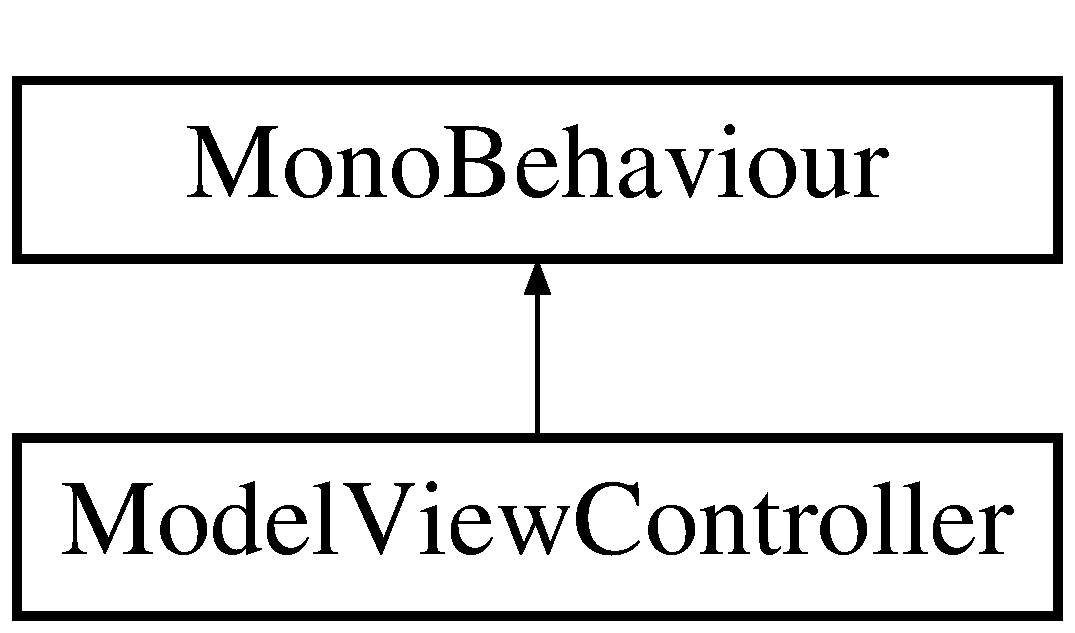
\includegraphics[height=2.000000cm]{class_model_view_controller}
\end{center}
\end{figure}
\subsection*{Public Member Functions}
\begin{DoxyCompactItemize}
\item 
void \hyperlink{class_model_view_controller_a733e3f93205ae7dea9e3c643a04174ea}{Change\+Type} (Behavior type)
\begin{DoxyCompactList}\small\item\em Changes the selected type of the M\+VC \end{DoxyCompactList}\item 
bool \hyperlink{class_model_view_controller_a9eba81ca552ecca21b7d58e66b12b952}{is\+Mouse\+Over\+Grid} ()
\begin{DoxyCompactList}\small\item\em Checks if the mouse is over the transform of the grid \end{DoxyCompactList}\item 
bool \hyperlink{class_model_view_controller_a2427ee5d98caea91251c69be3a29934a}{is\+Mouse\+Not\+Over\+Children} (bool select)
\begin{DoxyCompactList}\small\item\em Checks if the mouse is not over one of the Nodes \end{DoxyCompactList}\item 
void \hyperlink{class_model_view_controller_a598a752c88bbaf0f08f18e3a26a10671}{Hide\+Inspector} ()
\begin{DoxyCompactList}\small\item\em Function to hide the node and endge inspectors \end{DoxyCompactList}\item 
void \hyperlink{class_model_view_controller_a0131bdf2b008298e97229e2c729015d4}{Select\+Edge} (Game\+Object selected\+Edge)
\begin{DoxyCompactList}\small\item\em Tells the edge inspector to select the given object and tells the node inspector to deselect. \end{DoxyCompactList}\item 
void \hyperlink{class_model_view_controller_a08958c4f615ea68ec493fbb52139646c}{Add\+Node} (Behavior newbehavior, Vector2 pos)
\begin{DoxyCompactList}\small\item\em Adds a visual node to the diagram \end{DoxyCompactList}\item 
void \hyperlink{class_model_view_controller_a1a31ef775ee8e6090e99e0e09dff4eab}{Add\+Edge} (Vector2 pos)
\begin{DoxyCompactList}\small\item\em Adds a visual flow edge to the diagram \end{DoxyCompactList}\item 
void \hyperlink{class_model_view_controller_a1a64c20a275603c8c8352e82cc4c87ec}{Add\+State} (Vector2 pos)
\begin{DoxyCompactList}\small\item\em Adds a visual state edge to the diagram \end{DoxyCompactList}\end{DoxyCompactItemize}
\subsection*{Public Attributes}
\begin{DoxyCompactItemize}
\item 
\mbox{\Hypertarget{class_model_view_controller_abdf9d85627b8e6c2be4df28352354021}\label{class_model_view_controller_abdf9d85627b8e6c2be4df28352354021}} 
Game\+Object {\bfseries node\+Prefab}
\item 
\mbox{\Hypertarget{class_model_view_controller_a4e20a746b2c6d7b3081dc1ebf60d375b}\label{class_model_view_controller_a4e20a746b2c6d7b3081dc1ebf60d375b}} 
Game\+Object {\bfseries edge\+Prefab}
\item 
\mbox{\Hypertarget{class_model_view_controller_a3dac4afeed4f9f812ae6bccbe2b2af8d}\label{class_model_view_controller_a3dac4afeed4f9f812ae6bccbe2b2af8d}} 
Game\+Object {\bfseries state\+Prefab}
\item 
\mbox{\Hypertarget{class_model_view_controller_a3f01456e8d43bf45abdd67b9d2f2eca9}\label{class_model_view_controller_a3f01456e8d43bf45abdd67b9d2f2eca9}} 
Transform {\bfseries canvas}
\item 
\mbox{\Hypertarget{class_model_view_controller_a1855edfc4ec8960c03b4854c69c3b9fb}\label{class_model_view_controller_a1855edfc4ec8960c03b4854c69c3b9fb}} 
Transform {\bfseries view}
\item 
\mbox{\Hypertarget{class_model_view_controller_a8b41aa45d5ebf2fc8968d69f5213de72}\label{class_model_view_controller_a8b41aa45d5ebf2fc8968d69f5213de72}} 
Transform {\bfseries grid}
\item 
\mbox{\Hypertarget{class_model_view_controller_a7292985cf38fd72751d0dcdb91cc41b0}\label{class_model_view_controller_a7292985cf38fd72751d0dcdb91cc41b0}} 
Rect\+Transform {\bfseries grid\+Transform}
\item 
\mbox{\Hypertarget{class_model_view_controller_a1e4b34f4f1253772eb5d8cbca94c35bd}\label{class_model_view_controller_a1e4b34f4f1253772eb5d8cbca94c35bd}} 
Behavior {\bfseries selected\+Type} = Behavior.\+Mouse
\item 
\mbox{\Hypertarget{class_model_view_controller_ae03c4da99e654518796aad15c337aeed}\label{class_model_view_controller_ae03c4da99e654518796aad15c337aeed}} 
Scroll\+Rect {\bfseries scroll\+Rect}
\item 
\mbox{\Hypertarget{class_model_view_controller_ab2159253c4a9fa05433319858e20bfe4}\label{class_model_view_controller_ab2159253c4a9fa05433319858e20bfe4}} 
\hyperlink{class_model_controller}{Model\+Controller} {\bfseries model}
\item 
\mbox{\Hypertarget{class_model_view_controller_a39d8b10ab5d8b0acc9f3dc1997b50bf2}\label{class_model_view_controller_a39d8b10ab5d8b0acc9f3dc1997b50bf2}} 
Game\+Object {\bfseries temp\+Edge}
\item 
\mbox{\Hypertarget{class_model_view_controller_a1286a134fbcb061f3f6c0cacef0d932b}\label{class_model_view_controller_a1286a134fbcb061f3f6c0cacef0d932b}} 
Game\+Object {\bfseries temp\+State}
\item 
\mbox{\Hypertarget{class_model_view_controller_adc66a5588a24798d9f841b692ea9535a}\label{class_model_view_controller_adc66a5588a24798d9f841b692ea9535a}} 
bool {\bfseries something\+Selected} = false
\item 
\mbox{\Hypertarget{class_model_view_controller_a69ab61b3629af37235c4176dc4983259}\label{class_model_view_controller_a69ab61b3629af37235c4176dc4983259}} 
Game\+Object {\bfseries selected\+Object}
\item 
\mbox{\Hypertarget{class_model_view_controller_a01ebde35333857fff2556d966be1e71a}\label{class_model_view_controller_a01ebde35333857fff2556d966be1e71a}} 
\hyperlink{class_node_inspector}{Node\+Inspector} {\bfseries node\+Inspector}
\item 
\mbox{\Hypertarget{class_model_view_controller_a4f1f19194987a457784f16c46f5ca554}\label{class_model_view_controller_a4f1f19194987a457784f16c46f5ca554}} 
\hyperlink{class_edge_inspector}{Edge\+Inspector} {\bfseries edge\+Inspector}
\item 
\mbox{\Hypertarget{class_model_view_controller_a2570ca12086280f2e0880fe9ecfdf69d}\label{class_model_view_controller_a2570ca12086280f2e0880fe9ecfdf69d}} 
Game\+Object {\bfseries copied\+Node}
\item 
\mbox{\Hypertarget{class_model_view_controller_ac854a59175e809681769268b0efc9832}\label{class_model_view_controller_ac854a59175e809681769268b0efc9832}} 
Game\+Object {\bfseries temp\+Node}
\item 
\mbox{\Hypertarget{class_model_view_controller_adebc28b6cf6acb553f09d9c8238a6520}\label{class_model_view_controller_adebc28b6cf6acb553f09d9c8238a6520}} 
Rect\+Transform {\bfseries tab}
\end{DoxyCompactItemize}


\subsection{Detailed Description}
Model View Controller for the tool, links the visual (view) with the functional (model) elements of the diagrams 



\subsection{Member Function Documentation}
\mbox{\Hypertarget{class_model_view_controller_a1a31ef775ee8e6090e99e0e09dff4eab}\label{class_model_view_controller_a1a31ef775ee8e6090e99e0e09dff4eab}} 
\index{Model\+View\+Controller@{Model\+View\+Controller}!Add\+Edge@{Add\+Edge}}
\index{Add\+Edge@{Add\+Edge}!Model\+View\+Controller@{Model\+View\+Controller}}
\subsubsection{\texorpdfstring{Add\+Edge()}{AddEdge()}}
{\footnotesize\ttfamily void Model\+View\+Controller.\+Add\+Edge (\begin{DoxyParamCaption}\item[{Vector2}]{pos }\end{DoxyParamCaption})}



Adds a visual flow edge to the diagram 


\begin{DoxyParams}{Parameters}
{\em pos} & Starting position of the new flow edge\\
\hline
\end{DoxyParams}
\mbox{\Hypertarget{class_model_view_controller_a08958c4f615ea68ec493fbb52139646c}\label{class_model_view_controller_a08958c4f615ea68ec493fbb52139646c}} 
\index{Model\+View\+Controller@{Model\+View\+Controller}!Add\+Node@{Add\+Node}}
\index{Add\+Node@{Add\+Node}!Model\+View\+Controller@{Model\+View\+Controller}}
\subsubsection{\texorpdfstring{Add\+Node()}{AddNode()}}
{\footnotesize\ttfamily void Model\+View\+Controller.\+Add\+Node (\begin{DoxyParamCaption}\item[{Behavior}]{newbehavior,  }\item[{Vector2}]{pos }\end{DoxyParamCaption})}



Adds a visual node to the diagram 


\begin{DoxyParams}{Parameters}
{\em newbehavior} & The behavior of the new node\\
\hline
{\em pos} & The position of the new node\\
\hline
\end{DoxyParams}
\mbox{\Hypertarget{class_model_view_controller_a1a64c20a275603c8c8352e82cc4c87ec}\label{class_model_view_controller_a1a64c20a275603c8c8352e82cc4c87ec}} 
\index{Model\+View\+Controller@{Model\+View\+Controller}!Add\+State@{Add\+State}}
\index{Add\+State@{Add\+State}!Model\+View\+Controller@{Model\+View\+Controller}}
\subsubsection{\texorpdfstring{Add\+State()}{AddState()}}
{\footnotesize\ttfamily void Model\+View\+Controller.\+Add\+State (\begin{DoxyParamCaption}\item[{Vector2}]{pos }\end{DoxyParamCaption})}



Adds a visual state edge to the diagram 


\begin{DoxyParams}{Parameters}
{\em pos} & Starting position of the new state edge\\
\hline
\end{DoxyParams}
\mbox{\Hypertarget{class_model_view_controller_a733e3f93205ae7dea9e3c643a04174ea}\label{class_model_view_controller_a733e3f93205ae7dea9e3c643a04174ea}} 
\index{Model\+View\+Controller@{Model\+View\+Controller}!Change\+Type@{Change\+Type}}
\index{Change\+Type@{Change\+Type}!Model\+View\+Controller@{Model\+View\+Controller}}
\subsubsection{\texorpdfstring{Change\+Type()}{ChangeType()}}
{\footnotesize\ttfamily void Model\+View\+Controller.\+Change\+Type (\begin{DoxyParamCaption}\item[{Behavior}]{type }\end{DoxyParamCaption})}



Changes the selected type of the M\+VC 


\begin{DoxyParams}{Parameters}
{\em type} & The new type \\
\hline
\end{DoxyParams}
\mbox{\Hypertarget{class_model_view_controller_a598a752c88bbaf0f08f18e3a26a10671}\label{class_model_view_controller_a598a752c88bbaf0f08f18e3a26a10671}} 
\index{Model\+View\+Controller@{Model\+View\+Controller}!Hide\+Inspector@{Hide\+Inspector}}
\index{Hide\+Inspector@{Hide\+Inspector}!Model\+View\+Controller@{Model\+View\+Controller}}
\subsubsection{\texorpdfstring{Hide\+Inspector()}{HideInspector()}}
{\footnotesize\ttfamily void Model\+View\+Controller.\+Hide\+Inspector (\begin{DoxyParamCaption}{ }\end{DoxyParamCaption})}



Function to hide the node and endge inspectors 

\mbox{\Hypertarget{class_model_view_controller_a2427ee5d98caea91251c69be3a29934a}\label{class_model_view_controller_a2427ee5d98caea91251c69be3a29934a}} 
\index{Model\+View\+Controller@{Model\+View\+Controller}!is\+Mouse\+Not\+Over\+Children@{is\+Mouse\+Not\+Over\+Children}}
\index{is\+Mouse\+Not\+Over\+Children@{is\+Mouse\+Not\+Over\+Children}!Model\+View\+Controller@{Model\+View\+Controller}}
\subsubsection{\texorpdfstring{is\+Mouse\+Not\+Over\+Children()}{isMouseNotOverChildren()}}
{\footnotesize\ttfamily bool Model\+View\+Controller.\+is\+Mouse\+Not\+Over\+Children (\begin{DoxyParamCaption}\item[{bool}]{select }\end{DoxyParamCaption})}



Checks if the mouse is not over one of the Nodes 


\begin{DoxyParams}{Parameters}
{\em select} & If the mouse is over a node, should that node be selected? \\
\hline
\end{DoxyParams}
\begin{DoxyReturn}{Returns}
True if mouse is not over any children, False if the mouse is over a child 
\end{DoxyReturn}
\mbox{\Hypertarget{class_model_view_controller_a9eba81ca552ecca21b7d58e66b12b952}\label{class_model_view_controller_a9eba81ca552ecca21b7d58e66b12b952}} 
\index{Model\+View\+Controller@{Model\+View\+Controller}!is\+Mouse\+Over\+Grid@{is\+Mouse\+Over\+Grid}}
\index{is\+Mouse\+Over\+Grid@{is\+Mouse\+Over\+Grid}!Model\+View\+Controller@{Model\+View\+Controller}}
\subsubsection{\texorpdfstring{is\+Mouse\+Over\+Grid()}{isMouseOverGrid()}}
{\footnotesize\ttfamily bool Model\+View\+Controller.\+is\+Mouse\+Over\+Grid (\begin{DoxyParamCaption}{ }\end{DoxyParamCaption})}



Checks if the mouse is over the transform of the grid 

\begin{DoxyReturn}{Returns}
returns true if the mouse is over the grid and returns false if it is not
\end{DoxyReturn}
\mbox{\Hypertarget{class_model_view_controller_a0131bdf2b008298e97229e2c729015d4}\label{class_model_view_controller_a0131bdf2b008298e97229e2c729015d4}} 
\index{Model\+View\+Controller@{Model\+View\+Controller}!Select\+Edge@{Select\+Edge}}
\index{Select\+Edge@{Select\+Edge}!Model\+View\+Controller@{Model\+View\+Controller}}
\subsubsection{\texorpdfstring{Select\+Edge()}{SelectEdge()}}
{\footnotesize\ttfamily void Model\+View\+Controller.\+Select\+Edge (\begin{DoxyParamCaption}\item[{Game\+Object}]{selected\+Edge }\end{DoxyParamCaption})}



Tells the edge inspector to select the given object and tells the node inspector to deselect. 


\begin{DoxyParams}{Parameters}
{\em selected\+Edge} & The selected edge\\
\hline
\end{DoxyParams}


The documentation for this class was generated from the following file\+:\begin{DoxyCompactItemize}
\item 
Model\+View\+Controller.\+cs\end{DoxyCompactItemize}

\hypertarget{class_node_inspector}{}\section{Node\+Inspector Class Reference}
\label{class_node_inspector}\index{Node\+Inspector@{Node\+Inspector}}


The node inspector  


Inheritance diagram for Node\+Inspector\+:\begin{figure}[H]
\begin{center}
\leavevmode
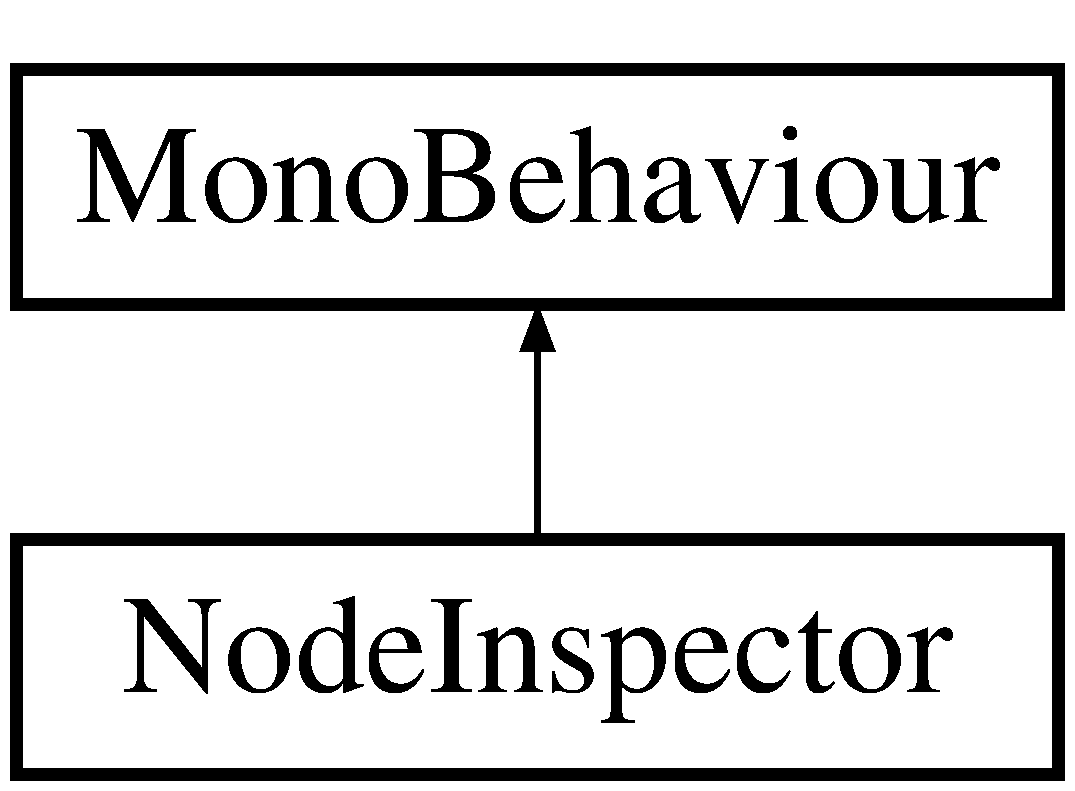
\includegraphics[height=2.000000cm]{class_node_inspector}
\end{center}
\end{figure}
\subsection*{Public Member Functions}
\begin{DoxyCompactItemize}
\item 
void \hyperlink{class_node_inspector_af14ce741da70a5d25865c72b6dc9291b}{Select} (Game\+Object selected\+Object)
\begin{DoxyCompactList}\small\item\em Selects given object in the node inspector \end{DoxyCompactList}\item 
void \hyperlink{class_node_inspector_a622010fcd39b4bee19087e238b9574d6}{Change\+Behavior} (Game\+Object selected\+Object)
\begin{DoxyCompactList}\small\item\em When the behavior of a Node changes while selected the inspector needs to update the content. \end{DoxyCompactList}\item 
void \hyperlink{class_node_inspector_a553862e69d98c5b5528871e1e3a18ad1}{Deselect} ()
\begin{DoxyCompactList}\small\item\em Clears selection of the Node Inspector. \end{DoxyCompactList}\item 
void \hyperlink{class_node_inspector_a652635a29e79966c2819eb20cc8bedc1}{Update\+Definitions} (Game\+Object selected\+Obj)
\begin{DoxyCompactList}\small\item\em Updates the options of the Type\+Of drop down. These options are the names of all other tabs in the editor. \end{DoxyCompactList}\item 
void \hyperlink{class_node_inspector_a7742d3d6c097ee5c2bdaea18741da3fe}{Update\+Text} ()
\begin{DoxyCompactList}\small\item\em Updates the Name of the currently selected node. \end{DoxyCompactList}\item 
void \hyperlink{class_node_inspector_a8e1c3d87fc6a3dc3addb0cf4eddfd7a6}{Update\+Type} ()
\begin{DoxyCompactList}\small\item\em Updates the Behavior component of the currently selected node. \end{DoxyCompactList}\item 
void \hyperlink{class_node_inspector_af94d04b7f31d5788591fa21f1c1ed1af}{Update\+Number} ()
\begin{DoxyCompactList}\small\item\em Updates the At component of the currently selected node. \end{DoxyCompactList}\item 
void \hyperlink{class_node_inspector_a5e707e8401204ddfab6e3468b007440f}{Update\+Capacity} ()
\begin{DoxyCompactList}\small\item\em Updates the Max component of the currently selected node. \end{DoxyCompactList}\item 
void \hyperlink{class_node_inspector_a700b7af667de0b1d5bbdca2051ae74c6}{Update\+Pull\+Mode} ()
\begin{DoxyCompactList}\small\item\em Updates the Act and How components of the currently selected node. \end{DoxyCompactList}\item 
void \hyperlink{class_node_inspector_a3886723916c36d8435c4c9c477a97040}{Update\+Activation} ()
\begin{DoxyCompactList}\small\item\em Updates the Activation component of the currently selected node. \end{DoxyCompactList}\item 
void \hyperlink{class_node_inspector_a3bf3fdb379bb3ed7acfb3099163538c4}{Update\+IO} ()
\begin{DoxyCompactList}\small\item\em Updates the In Out component of the currently selected node. \end{DoxyCompactList}\item 
void \hyperlink{class_node_inspector_ab378830e6c5353dc122bf5a99a30cb3a}{Update\+Add} ()
\begin{DoxyCompactList}\small\item\em Updates the Add component of the currently selected node. \end{DoxyCompactList}\item 
void \hyperlink{class_node_inspector_acbb1e1d49e8e382ea41c9685bb31f978}{Update\+Of\+Type} ()
\begin{DoxyCompactList}\small\item\em Updates the Of\+Type component of the currently selected node. \end{DoxyCompactList}\item 
void \hyperlink{class_node_inspector_a7d2d42f0b36ed545ee032cce4373ac82}{Update\+Position} ()
\begin{DoxyCompactList}\small\item\em Updates the position of the selected node \end{DoxyCompactList}\end{DoxyCompactItemize}
\subsection*{Public Attributes}
\begin{DoxyCompactItemize}
\item 
\mbox{\Hypertarget{class_node_inspector_a1623fe9201c6da160d2aa1733470f0ed}\label{class_node_inspector_a1623fe9201c6da160d2aa1733470f0ed}} 
Transform {\bfseries canvas}
\item 
\mbox{\Hypertarget{class_node_inspector_a32850b84ea0bca6d00e3e909750e462f}\label{class_node_inspector_a32850b84ea0bca6d00e3e909750e462f}} 
Game\+Object {\bfseries content}
\item 
\mbox{\Hypertarget{class_node_inspector_a7655520eb958764ddd84bd13fdcb21f2}\label{class_node_inspector_a7655520eb958764ddd84bd13fdcb21f2}} 
\hyperlink{class_model_controller}{Model\+Controller} {\bfseries mc}
\item 
\mbox{\Hypertarget{class_node_inspector_a18f38b14be386f8d49f1d7b27945f765}\label{class_node_inspector_a18f38b14be386f8d49f1d7b27945f765}} 
Game\+Object {\bfseries selected\+Node}
\item 
\mbox{\Hypertarget{class_node_inspector_aa46d142d06db8c09f421c1d8c8298565}\label{class_node_inspector_aa46d142d06db8c09f421c1d8c8298565}} 
Game\+Object {\bfseries at\+Field}
\item 
\mbox{\Hypertarget{class_node_inspector_ab58340267ebb6e122c86ad1558ef5126}\label{class_node_inspector_ab58340267ebb6e122c86ad1558ef5126}} 
Game\+Object {\bfseries max\+Field}
\item 
\mbox{\Hypertarget{class_node_inspector_a7e3974940fa9baab934bbcd83a0b10cf}\label{class_node_inspector_a7e3974940fa9baab934bbcd83a0b10cf}} 
Game\+Object {\bfseries add\+Field}
\item 
\mbox{\Hypertarget{class_node_inspector_aac889ecd05eb9ac0b86083b9d59f3064}\label{class_node_inspector_aac889ecd05eb9ac0b86083b9d59f3064}} 
Game\+Object {\bfseries of\+Type\+Field}
\item 
\mbox{\Hypertarget{class_node_inspector_a5f8dd9bd7ae292bccfa7a407c762c58a}\label{class_node_inspector_a5f8dd9bd7ae292bccfa7a407c762c58a}} 
Input\+Field {\bfseries label}
\item 
\mbox{\Hypertarget{class_node_inspector_aeb4e35b5aaf37b598d1c68af0f01971c}\label{class_node_inspector_aeb4e35b5aaf37b598d1c68af0f01971c}} 
Input\+Field {\bfseries at}
\item 
\mbox{\Hypertarget{class_node_inspector_af7f1d559ada7ac0aada6f9894d634d2e}\label{class_node_inspector_af7f1d559ada7ac0aada6f9894d634d2e}} 
Input\+Field {\bfseries max}
\item 
\mbox{\Hypertarget{class_node_inspector_ae969c1cf7237b1ceb4315169c7b4d60d}\label{class_node_inspector_ae969c1cf7237b1ceb4315169c7b4d60d}} 
Input\+Field {\bfseries add}
\item 
\mbox{\Hypertarget{class_node_inspector_a21c482f182e545d7704c38f2fb489c29}\label{class_node_inspector_a21c482f182e545d7704c38f2fb489c29}} 
Input\+Field {\bfseries positionx}
\item 
\mbox{\Hypertarget{class_node_inspector_ae6cc2edfe5015761e34a2b8caa662ec7}\label{class_node_inspector_ae6cc2edfe5015761e34a2b8caa662ec7}} 
Input\+Field {\bfseries positiony}
\item 
\mbox{\Hypertarget{class_node_inspector_aa074f71f1f890c09ba823eda0c608523}\label{class_node_inspector_aa074f71f1f890c09ba823eda0c608523}} 
Dropdown {\bfseries whendd}
\item 
\mbox{\Hypertarget{class_node_inspector_ada4f256c5deb0acda36e18f0b4c27137}\label{class_node_inspector_ada4f256c5deb0acda36e18f0b4c27137}} 
Dropdown {\bfseries actdd}
\item 
\mbox{\Hypertarget{class_node_inspector_ae02587c2ce15aea863916cd9db10767b}\label{class_node_inspector_ae02587c2ce15aea863916cd9db10767b}} 
Dropdown {\bfseries howdd}
\item 
\mbox{\Hypertarget{class_node_inspector_aaad59cf9222edab92590757567b2f893}\label{class_node_inspector_aaad59cf9222edab92590757567b2f893}} 
Dropdown {\bfseries behaviordd}
\item 
\mbox{\Hypertarget{class_node_inspector_a3c57564ec2eb96805ab76844f1d7b1be}\label{class_node_inspector_a3c57564ec2eb96805ab76844f1d7b1be}} 
Dropdown {\bfseries inoutdd}
\item 
\mbox{\Hypertarget{class_node_inspector_a69f86146243d61986410aaa6dd3c106b}\label{class_node_inspector_a69f86146243d61986410aaa6dd3c106b}} 
Dropdown {\bfseries of\+Typedd}
\item 
\mbox{\Hypertarget{class_node_inspector_a68b3699c849226225b67993b588792c1}\label{class_node_inspector_a68b3699c849226225b67993b588792c1}} 
string {\bfseries active\+Tab\+Name}
\end{DoxyCompactItemize}


\subsection{Detailed Description}
The node inspector 



\subsection{Member Function Documentation}
\mbox{\Hypertarget{class_node_inspector_a622010fcd39b4bee19087e238b9574d6}\label{class_node_inspector_a622010fcd39b4bee19087e238b9574d6}} 
\index{Node\+Inspector@{Node\+Inspector}!Change\+Behavior@{Change\+Behavior}}
\index{Change\+Behavior@{Change\+Behavior}!Node\+Inspector@{Node\+Inspector}}
\subsubsection{\texorpdfstring{Change\+Behavior()}{ChangeBehavior()}}
{\footnotesize\ttfamily void Node\+Inspector.\+Change\+Behavior (\begin{DoxyParamCaption}\item[{Game\+Object}]{selected\+Object }\end{DoxyParamCaption})}



When the behavior of a Node changes while selected the inspector needs to update the content. 


\begin{DoxyParams}{Parameters}
{\em selected\+Object} & The selected object. \\
\hline
\end{DoxyParams}
\mbox{\Hypertarget{class_node_inspector_a553862e69d98c5b5528871e1e3a18ad1}\label{class_node_inspector_a553862e69d98c5b5528871e1e3a18ad1}} 
\index{Node\+Inspector@{Node\+Inspector}!Deselect@{Deselect}}
\index{Deselect@{Deselect}!Node\+Inspector@{Node\+Inspector}}
\subsubsection{\texorpdfstring{Deselect()}{Deselect()}}
{\footnotesize\ttfamily void Node\+Inspector.\+Deselect (\begin{DoxyParamCaption}{ }\end{DoxyParamCaption})}



Clears selection of the Node Inspector. 

\mbox{\Hypertarget{class_node_inspector_af14ce741da70a5d25865c72b6dc9291b}\label{class_node_inspector_af14ce741da70a5d25865c72b6dc9291b}} 
\index{Node\+Inspector@{Node\+Inspector}!Select@{Select}}
\index{Select@{Select}!Node\+Inspector@{Node\+Inspector}}
\subsubsection{\texorpdfstring{Select()}{Select()}}
{\footnotesize\ttfamily void Node\+Inspector.\+Select (\begin{DoxyParamCaption}\item[{Game\+Object}]{selected\+Object }\end{DoxyParamCaption})}



Selects given object in the node inspector 


\begin{DoxyParams}{Parameters}
{\em selected\+Object} & the object that needs to be inspected \\
\hline
\end{DoxyParams}
\mbox{\Hypertarget{class_node_inspector_a3886723916c36d8435c4c9c477a97040}\label{class_node_inspector_a3886723916c36d8435c4c9c477a97040}} 
\index{Node\+Inspector@{Node\+Inspector}!Update\+Activation@{Update\+Activation}}
\index{Update\+Activation@{Update\+Activation}!Node\+Inspector@{Node\+Inspector}}
\subsubsection{\texorpdfstring{Update\+Activation()}{UpdateActivation()}}
{\footnotesize\ttfamily void Node\+Inspector.\+Update\+Activation (\begin{DoxyParamCaption}{ }\end{DoxyParamCaption})}



Updates the Activation component of the currently selected node. 

\mbox{\Hypertarget{class_node_inspector_ab378830e6c5353dc122bf5a99a30cb3a}\label{class_node_inspector_ab378830e6c5353dc122bf5a99a30cb3a}} 
\index{Node\+Inspector@{Node\+Inspector}!Update\+Add@{Update\+Add}}
\index{Update\+Add@{Update\+Add}!Node\+Inspector@{Node\+Inspector}}
\subsubsection{\texorpdfstring{Update\+Add()}{UpdateAdd()}}
{\footnotesize\ttfamily void Node\+Inspector.\+Update\+Add (\begin{DoxyParamCaption}{ }\end{DoxyParamCaption})}



Updates the Add component of the currently selected node. 

\mbox{\Hypertarget{class_node_inspector_a5e707e8401204ddfab6e3468b007440f}\label{class_node_inspector_a5e707e8401204ddfab6e3468b007440f}} 
\index{Node\+Inspector@{Node\+Inspector}!Update\+Capacity@{Update\+Capacity}}
\index{Update\+Capacity@{Update\+Capacity}!Node\+Inspector@{Node\+Inspector}}
\subsubsection{\texorpdfstring{Update\+Capacity()}{UpdateCapacity()}}
{\footnotesize\ttfamily void Node\+Inspector.\+Update\+Capacity (\begin{DoxyParamCaption}{ }\end{DoxyParamCaption})}



Updates the Max component of the currently selected node. 

\mbox{\Hypertarget{class_node_inspector_a652635a29e79966c2819eb20cc8bedc1}\label{class_node_inspector_a652635a29e79966c2819eb20cc8bedc1}} 
\index{Node\+Inspector@{Node\+Inspector}!Update\+Definitions@{Update\+Definitions}}
\index{Update\+Definitions@{Update\+Definitions}!Node\+Inspector@{Node\+Inspector}}
\subsubsection{\texorpdfstring{Update\+Definitions()}{UpdateDefinitions()}}
{\footnotesize\ttfamily void Node\+Inspector.\+Update\+Definitions (\begin{DoxyParamCaption}\item[{Game\+Object}]{selected\+Obj }\end{DoxyParamCaption})}



Updates the options of the Type\+Of drop down. These options are the names of all other tabs in the editor. 


\begin{DoxyParams}{Parameters}
{\em selected\+Obj} & The current selected object used to set the default value of the drop down to whatever the selected object already has \\
\hline
\end{DoxyParams}
\mbox{\Hypertarget{class_node_inspector_a3bf3fdb379bb3ed7acfb3099163538c4}\label{class_node_inspector_a3bf3fdb379bb3ed7acfb3099163538c4}} 
\index{Node\+Inspector@{Node\+Inspector}!Update\+IO@{Update\+IO}}
\index{Update\+IO@{Update\+IO}!Node\+Inspector@{Node\+Inspector}}
\subsubsection{\texorpdfstring{Update\+I\+O()}{UpdateIO()}}
{\footnotesize\ttfamily void Node\+Inspector.\+Update\+IO (\begin{DoxyParamCaption}{ }\end{DoxyParamCaption})}



Updates the In Out component of the currently selected node. 

\mbox{\Hypertarget{class_node_inspector_af94d04b7f31d5788591fa21f1c1ed1af}\label{class_node_inspector_af94d04b7f31d5788591fa21f1c1ed1af}} 
\index{Node\+Inspector@{Node\+Inspector}!Update\+Number@{Update\+Number}}
\index{Update\+Number@{Update\+Number}!Node\+Inspector@{Node\+Inspector}}
\subsubsection{\texorpdfstring{Update\+Number()}{UpdateNumber()}}
{\footnotesize\ttfamily void Node\+Inspector.\+Update\+Number (\begin{DoxyParamCaption}{ }\end{DoxyParamCaption})}



Updates the At component of the currently selected node. 

\mbox{\Hypertarget{class_node_inspector_acbb1e1d49e8e382ea41c9685bb31f978}\label{class_node_inspector_acbb1e1d49e8e382ea41c9685bb31f978}} 
\index{Node\+Inspector@{Node\+Inspector}!Update\+Of\+Type@{Update\+Of\+Type}}
\index{Update\+Of\+Type@{Update\+Of\+Type}!Node\+Inspector@{Node\+Inspector}}
\subsubsection{\texorpdfstring{Update\+Of\+Type()}{UpdateOfType()}}
{\footnotesize\ttfamily void Node\+Inspector.\+Update\+Of\+Type (\begin{DoxyParamCaption}{ }\end{DoxyParamCaption})}



Updates the Of\+Type component of the currently selected node. 

\mbox{\Hypertarget{class_node_inspector_a7d2d42f0b36ed545ee032cce4373ac82}\label{class_node_inspector_a7d2d42f0b36ed545ee032cce4373ac82}} 
\index{Node\+Inspector@{Node\+Inspector}!Update\+Position@{Update\+Position}}
\index{Update\+Position@{Update\+Position}!Node\+Inspector@{Node\+Inspector}}
\subsubsection{\texorpdfstring{Update\+Position()}{UpdatePosition()}}
{\footnotesize\ttfamily void Node\+Inspector.\+Update\+Position (\begin{DoxyParamCaption}{ }\end{DoxyParamCaption})}



Updates the position of the selected node 

\mbox{\Hypertarget{class_node_inspector_a700b7af667de0b1d5bbdca2051ae74c6}\label{class_node_inspector_a700b7af667de0b1d5bbdca2051ae74c6}} 
\index{Node\+Inspector@{Node\+Inspector}!Update\+Pull\+Mode@{Update\+Pull\+Mode}}
\index{Update\+Pull\+Mode@{Update\+Pull\+Mode}!Node\+Inspector@{Node\+Inspector}}
\subsubsection{\texorpdfstring{Update\+Pull\+Mode()}{UpdatePullMode()}}
{\footnotesize\ttfamily void Node\+Inspector.\+Update\+Pull\+Mode (\begin{DoxyParamCaption}{ }\end{DoxyParamCaption})}



Updates the Act and How components of the currently selected node. 

\mbox{\Hypertarget{class_node_inspector_a7742d3d6c097ee5c2bdaea18741da3fe}\label{class_node_inspector_a7742d3d6c097ee5c2bdaea18741da3fe}} 
\index{Node\+Inspector@{Node\+Inspector}!Update\+Text@{Update\+Text}}
\index{Update\+Text@{Update\+Text}!Node\+Inspector@{Node\+Inspector}}
\subsubsection{\texorpdfstring{Update\+Text()}{UpdateText()}}
{\footnotesize\ttfamily void Node\+Inspector.\+Update\+Text (\begin{DoxyParamCaption}{ }\end{DoxyParamCaption})}



Updates the Name of the currently selected node. 

\mbox{\Hypertarget{class_node_inspector_a8e1c3d87fc6a3dc3addb0cf4eddfd7a6}\label{class_node_inspector_a8e1c3d87fc6a3dc3addb0cf4eddfd7a6}} 
\index{Node\+Inspector@{Node\+Inspector}!Update\+Type@{Update\+Type}}
\index{Update\+Type@{Update\+Type}!Node\+Inspector@{Node\+Inspector}}
\subsubsection{\texorpdfstring{Update\+Type()}{UpdateType()}}
{\footnotesize\ttfamily void Node\+Inspector.\+Update\+Type (\begin{DoxyParamCaption}{ }\end{DoxyParamCaption})}



Updates the Behavior component of the currently selected node. 



The documentation for this class was generated from the following file\+:\begin{DoxyCompactItemize}
\item 
Node\+Inspector.\+cs\end{DoxyCompactItemize}

\hypertarget{class_open_file_script}{}\section{Open\+File\+Script Class Reference}
\label{class_open_file_script}\index{Open\+File\+Script@{Open\+File\+Script}}


Opens a micro-\/machinations file and creates a visual diagram from it  


Inheritance diagram for Open\+File\+Script\+:\begin{figure}[H]
\begin{center}
\leavevmode
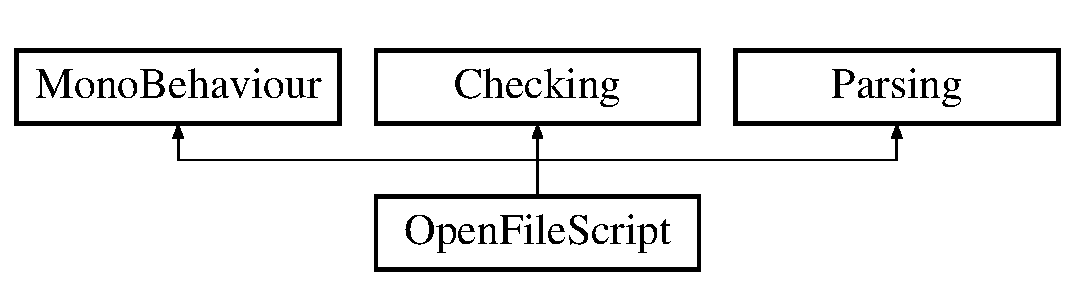
\includegraphics[height=2.000000cm]{class_open_file_script}
\end{center}
\end{figure}
\subsection*{Public Member Functions}
\begin{DoxyCompactItemize}
\item 
void \hyperlink{class_open_file_script_a94b7ce5bc20da9a8be4322c1eb53fd75}{receive} (M\+M.\+Parser.\+Parser\+Message message)
\begin{DoxyCompactList}\small\item\em Receives error/warning messages from the parser T\+O\+DO\+: Use the tools own console instead of unity debugger. \end{DoxyCompactList}\item 
void \hyperlink{class_open_file_script_aa2396d19a7620be7dd7e327865fc9501}{receive} (M\+M.\+Runtime.\+Checker\+Message message)
\begin{DoxyCompactList}\small\item\em Receives error/warning messages from the runtime model T\+O\+DO\+: Use the tools own console instead of unity debugger. \end{DoxyCompactList}\end{DoxyCompactItemize}
\subsection*{Public Attributes}
\begin{DoxyCompactItemize}
\item 
\mbox{\Hypertarget{class_open_file_script_a350ae639143fb60f7ae57729656dc12d}\label{class_open_file_script_a350ae639143fb60f7ae57729656dc12d}} 
Unity\+Engine.\+U\+I.\+Button {\bfseries your\+Button}
\item 
\mbox{\Hypertarget{class_open_file_script_aee899fa35c56029fae604c45669e7b3d}\label{class_open_file_script_aee899fa35c56029fae604c45669e7b3d}} 
string {\bfseries file}
\item 
\mbox{\Hypertarget{class_open_file_script_af58aa31852b32428025ff87c9b1a4166}\label{class_open_file_script_af58aa31852b32428025ff87c9b1a4166}} 
string {\bfseries path} = null
\item 
\mbox{\Hypertarget{class_open_file_script_a139b85dfc4933e180ed34cd7152bd19a}\label{class_open_file_script_a139b85dfc4933e180ed34cd7152bd19a}} 
Program {\bfseries program}
\item 
\mbox{\Hypertarget{class_open_file_script_ab7b1ffe8e6c4fb6e38c8969e664728b5}\label{class_open_file_script_ab7b1ffe8e6c4fb6e38c8969e664728b5}} 
\hyperlink{class_tab_manager}{Tab\+Manager} {\bfseries tabman}
\item 
\mbox{\Hypertarget{class_open_file_script_a8cdf361b25e255e1c4b810dcd94f6893}\label{class_open_file_script_a8cdf361b25e255e1c4b810dcd94f6893}} 
Game\+Object {\bfseries tab}
\item 
\mbox{\Hypertarget{class_open_file_script_aef81c0cdf4e8ffa21ab35a6544f69d6c}\label{class_open_file_script_aef81c0cdf4e8ffa21ab35a6544f69d6c}} 
Game\+Object {\bfseries temp\+Node}
\item 
\mbox{\Hypertarget{class_open_file_script_ab553f0a078a9f4a6bb3428123da5f376}\label{class_open_file_script_ab553f0a078a9f4a6bb3428123da5f376}} 
\hyperlink{class_model_controller}{Model\+Controller} {\bfseries mc}
\item 
\mbox{\Hypertarget{class_open_file_script_a35f21e09c99790fc9d874a90e4313ed5}\label{class_open_file_script_a35f21e09c99790fc9d874a90e4313ed5}} 
List$<$ Game\+Object $>$ {\bfseries tabs} = new List$<$Game\+Object$>$()
\end{DoxyCompactItemize}


\subsection{Detailed Description}
Opens a micro-\/machinations file and creates a visual diagram from it 



\subsection{Member Function Documentation}
\mbox{\Hypertarget{class_open_file_script_a94b7ce5bc20da9a8be4322c1eb53fd75}\label{class_open_file_script_a94b7ce5bc20da9a8be4322c1eb53fd75}} 
\index{Open\+File\+Script@{Open\+File\+Script}!receive@{receive}}
\index{receive@{receive}!Open\+File\+Script@{Open\+File\+Script}}
\subsubsection{\texorpdfstring{receive()}{receive()}\hspace{0.1cm}{\footnotesize\ttfamily [1/2]}}
{\footnotesize\ttfamily void Open\+File\+Script.\+receive (\begin{DoxyParamCaption}\item[{M\+M.\+Parser.\+Parser\+Message}]{message }\end{DoxyParamCaption})}



Receives error/warning messages from the parser T\+O\+DO\+: Use the tools own console instead of unity debugger. 


\begin{DoxyParams}{Parameters}
{\em message} & The error message received\\
\hline
\end{DoxyParams}
\mbox{\Hypertarget{class_open_file_script_aa2396d19a7620be7dd7e327865fc9501}\label{class_open_file_script_aa2396d19a7620be7dd7e327865fc9501}} 
\index{Open\+File\+Script@{Open\+File\+Script}!receive@{receive}}
\index{receive@{receive}!Open\+File\+Script@{Open\+File\+Script}}
\subsubsection{\texorpdfstring{receive()}{receive()}\hspace{0.1cm}{\footnotesize\ttfamily [2/2]}}
{\footnotesize\ttfamily void Open\+File\+Script.\+receive (\begin{DoxyParamCaption}\item[{M\+M.\+Runtime.\+Checker\+Message}]{message }\end{DoxyParamCaption})}



Receives error/warning messages from the runtime model T\+O\+DO\+: Use the tools own console instead of unity debugger. 


\begin{DoxyParams}{Parameters}
{\em message} & The error message received\\
\hline
\end{DoxyParams}


The documentation for this class was generated from the following file\+:\begin{DoxyCompactItemize}
\item 
Open\+File\+Script.\+cs\end{DoxyCompactItemize}

\hypertarget{class_select_edge_button}{}\section{Select\+Edge\+Button Class Reference}
\label{class_select_edge_button}\index{Select\+Edge\+Button@{Select\+Edge\+Button}}


Visual Edge Object logic  


Inheritance diagram for Select\+Edge\+Button\+:\begin{figure}[H]
\begin{center}
\leavevmode
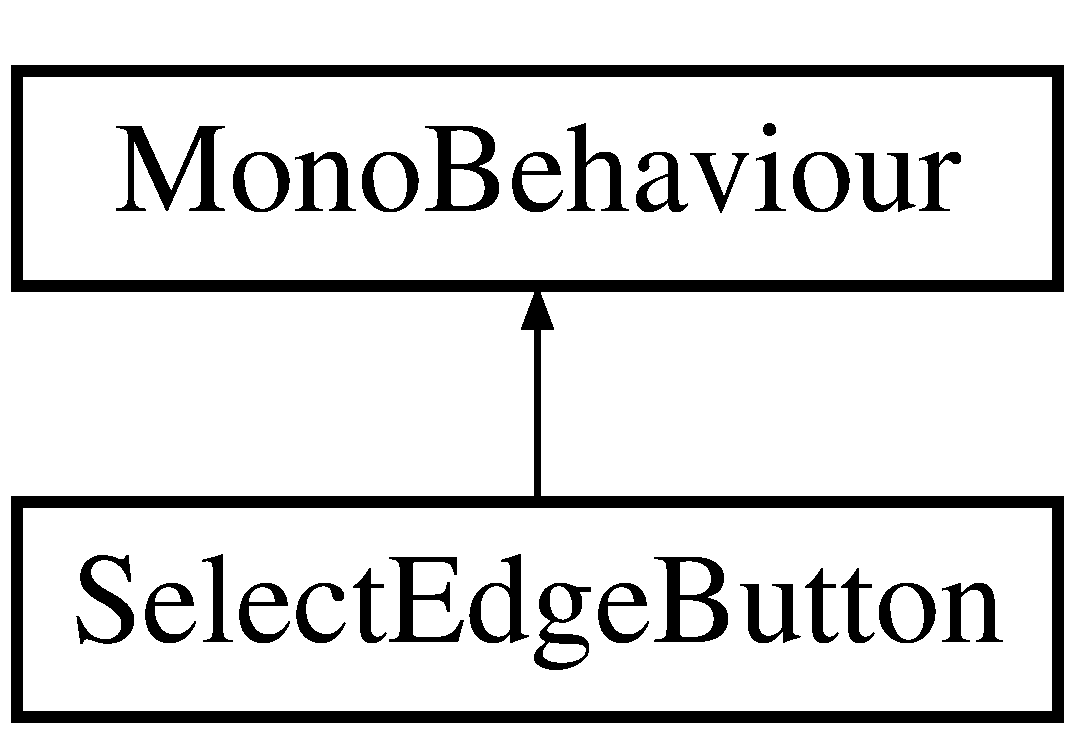
\includegraphics[height=2.000000cm]{class_select_edge_button}
\end{center}
\end{figure}
\subsection*{Public Member Functions}
\begin{DoxyCompactItemize}
\item 
void \hyperlink{class_select_edge_button_a1feacae4681c9223e93212b399a45804}{Add\+Edge\+Point} (Vector2 new\+Point, Game\+Object parent)
\begin{DoxyCompactList}\small\item\em Adds a new corner point to the edge T\+O\+DO\+: Corner points should be moveable \end{DoxyCompactList}\item 
void \hyperlink{class_select_edge_button_adba216e2255a885ba68f71ab755050e6}{Stretch} (Rect\+Transform \+\_\+sprite, Vector2 \+\_\+initial\+Position, Vector2 \+\_\+final\+Position)
\begin{DoxyCompactList}\small\item\em Stretches the edge image between two points (Important\+: Edges use Raw\+Images for UV management!) \end{DoxyCompactList}\item 
void \hyperlink{class_select_edge_button_a95682addf9c0dc548bdbec0677295275}{Stop\+Current\+Edge} ()
\begin{DoxyCompactList}\small\item\em Completes the edge (stops stretching to mouse) \end{DoxyCompactList}\item 
void \hyperlink{class_select_edge_button_a2955591ac3928b72e096de918c98f9e4}{Deselect} ()
\begin{DoxyCompactList}\small\item\em deselects \end{DoxyCompactList}\item 
bool \hyperlink{class_select_edge_button_a2931dd33f05961306aba6cdf535a597a}{Update\+Source} (string new\+Source\+Name)
\begin{DoxyCompactList}\small\item\em Updates the source of this edge \end{DoxyCompactList}\item 
bool \hyperlink{class_select_edge_button_a3a394258288e816eb5c06e6608edad4a}{Update\+Target} (string new\+Target\+Name)
\begin{DoxyCompactList}\small\item\em Updates the target node of this edge \end{DoxyCompactList}\end{DoxyCompactItemize}
\subsection*{Public Attributes}
\begin{DoxyCompactItemize}
\item 
\mbox{\Hypertarget{class_select_edge_button_ad8091eded4e5867a05a3d8ca5661986c}\label{class_select_edge_button_ad8091eded4e5867a05a3d8ca5661986c}} 
List$<$ Rect\+Transform $>$ {\bfseries edge\+Corners}
\item 
\mbox{\Hypertarget{class_select_edge_button_aa266ecdd7eaa7905573c9ea51672c346}\label{class_select_edge_button_aa266ecdd7eaa7905573c9ea51672c346}} 
Button {\bfseries your\+Button}
\item 
\mbox{\Hypertarget{class_select_edge_button_a61a55560653b35c10c98a23d76752218}\label{class_select_edge_button_a61a55560653b35c10c98a23d76752218}} 
Behavior {\bfseries type}
\item 
\mbox{\Hypertarget{class_select_edge_button_a7e39634ae2b028aec4dedcf870423a7d}\label{class_select_edge_button_a7e39634ae2b028aec4dedcf870423a7d}} 
Rect\+Transform {\bfseries line\+Image}
\item 
\mbox{\Hypertarget{class_select_edge_button_adb4a2fb2758a17b836baf88968e30ba5}\label{class_select_edge_button_adb4a2fb2758a17b836baf88968e30ba5}} 
Rect\+Transform {\bfseries corner\+Image}
\item 
\mbox{\Hypertarget{class_select_edge_button_afe01a333d58c771cd8d5b04b6c68c24d}\label{class_select_edge_button_afe01a333d58c771cd8d5b04b6c68c24d}} 
Rect\+Transform {\bfseries temp\+Edge}
\item 
\mbox{\Hypertarget{class_select_edge_button_add0fdd522d721462d82dc29803b00c51}\label{class_select_edge_button_add0fdd522d721462d82dc29803b00c51}} 
Sprite {\bfseries corner\+Sprite}
\item 
\mbox{\Hypertarget{class_select_edge_button_a52992d67a442bc9b14b6628fbfa6fd16}\label{class_select_edge_button_a52992d67a442bc9b14b6628fbfa6fd16}} 
Transform {\bfseries content}
\item 
\mbox{\Hypertarget{class_select_edge_button_a5bad131a282de8f14427fa3a3e93e588}\label{class_select_edge_button_a5bad131a282de8f14427fa3a3e93e588}} 
bool {\bfseries is\+Selected} = false
\item 
\mbox{\Hypertarget{class_select_edge_button_a068915d3ba018eb2c831bd727be5b2ea}\label{class_select_edge_button_a068915d3ba018eb2c831bd727be5b2ea}} 
M\+M.\+Model.\+Edge {\bfseries idedge}
\item 
\mbox{\Hypertarget{class_select_edge_button_ae2195894dd4f4fe1511405f1966eaa19}\label{class_select_edge_button_ae2195894dd4f4fe1511405f1966eaa19}} 
Text {\bfseries label}
\item 
\mbox{\Hypertarget{class_select_edge_button_a8116f80bd330d6d7c8c8481155fe0e42}\label{class_select_edge_button_a8116f80bd330d6d7c8c8481155fe0e42}} 
Text {\bfseries exp}
\item 
\mbox{\Hypertarget{class_select_edge_button_a61e8292864e91cc8418ba59719eae4a4}\label{class_select_edge_button_a61e8292864e91cc8418ba59719eae4a4}} 
string {\bfseries source}
\item 
\mbox{\Hypertarget{class_select_edge_button_a7e3535b7b32c7201fdf00f4befd514cd}\label{class_select_edge_button_a7e3535b7b32c7201fdf00f4befd514cd}} 
string {\bfseries target}
\item 
\mbox{\Hypertarget{class_select_edge_button_a1e1610e8f5ef52f41346973f160c0e7b}\label{class_select_edge_button_a1e1610e8f5ef52f41346973f160c0e7b}} 
Game\+Object {\bfseries source\+Obj} = null
\item 
\mbox{\Hypertarget{class_select_edge_button_ab0f5e1f7057fe3fa68c424174c2fe7b3}\label{class_select_edge_button_ab0f5e1f7057fe3fa68c424174c2fe7b3}} 
Game\+Object {\bfseries target\+Obj} = null
\item 
\mbox{\Hypertarget{class_select_edge_button_ae5b245dd838ecae0377648102ba4763a}\label{class_select_edge_button_ae5b245dd838ecae0377648102ba4763a}} 
Rect\+Transform {\bfseries source\+Corner} = null
\item 
\mbox{\Hypertarget{class_select_edge_button_adf0325406dd21f8b89a6b57892ef56ee}\label{class_select_edge_button_adf0325406dd21f8b89a6b57892ef56ee}} 
Rect\+Transform {\bfseries target\+Corner} = null
\item 
\mbox{\Hypertarget{class_select_edge_button_a56a6d857fbec1524dbc4067a7843152f}\label{class_select_edge_button_a56a6d857fbec1524dbc4067a7843152f}} 
Rect\+Transform {\bfseries edge\+Arrow}
\end{DoxyCompactItemize}


\subsection{Detailed Description}
Visual Edge Object logic 



\subsection{Member Function Documentation}
\mbox{\Hypertarget{class_select_edge_button_a1feacae4681c9223e93212b399a45804}\label{class_select_edge_button_a1feacae4681c9223e93212b399a45804}} 
\index{Select\+Edge\+Button@{Select\+Edge\+Button}!Add\+Edge\+Point@{Add\+Edge\+Point}}
\index{Add\+Edge\+Point@{Add\+Edge\+Point}!Select\+Edge\+Button@{Select\+Edge\+Button}}
\subsubsection{\texorpdfstring{Add\+Edge\+Point()}{AddEdgePoint()}}
{\footnotesize\ttfamily void Select\+Edge\+Button.\+Add\+Edge\+Point (\begin{DoxyParamCaption}\item[{Vector2}]{new\+Point,  }\item[{Game\+Object}]{parent }\end{DoxyParamCaption})}



Adds a new corner point to the edge T\+O\+DO\+: Corner points should be moveable 


\begin{DoxyParams}{Parameters}
{\em new\+Point} & Position of the new point\\
\hline
{\em parent} & Parent of the new point (important for target/source)\\
\hline
\end{DoxyParams}
\mbox{\Hypertarget{class_select_edge_button_a2955591ac3928b72e096de918c98f9e4}\label{class_select_edge_button_a2955591ac3928b72e096de918c98f9e4}} 
\index{Select\+Edge\+Button@{Select\+Edge\+Button}!Deselect@{Deselect}}
\index{Deselect@{Deselect}!Select\+Edge\+Button@{Select\+Edge\+Button}}
\subsubsection{\texorpdfstring{Deselect()}{Deselect()}}
{\footnotesize\ttfamily void Select\+Edge\+Button.\+Deselect (\begin{DoxyParamCaption}{ }\end{DoxyParamCaption})}



deselects 

\mbox{\Hypertarget{class_select_edge_button_a95682addf9c0dc548bdbec0677295275}\label{class_select_edge_button_a95682addf9c0dc548bdbec0677295275}} 
\index{Select\+Edge\+Button@{Select\+Edge\+Button}!Stop\+Current\+Edge@{Stop\+Current\+Edge}}
\index{Stop\+Current\+Edge@{Stop\+Current\+Edge}!Select\+Edge\+Button@{Select\+Edge\+Button}}
\subsubsection{\texorpdfstring{Stop\+Current\+Edge()}{StopCurrentEdge()}}
{\footnotesize\ttfamily void Select\+Edge\+Button.\+Stop\+Current\+Edge (\begin{DoxyParamCaption}{ }\end{DoxyParamCaption})}



Completes the edge (stops stretching to mouse) 

\mbox{\Hypertarget{class_select_edge_button_adba216e2255a885ba68f71ab755050e6}\label{class_select_edge_button_adba216e2255a885ba68f71ab755050e6}} 
\index{Select\+Edge\+Button@{Select\+Edge\+Button}!Stretch@{Stretch}}
\index{Stretch@{Stretch}!Select\+Edge\+Button@{Select\+Edge\+Button}}
\subsubsection{\texorpdfstring{Stretch()}{Stretch()}}
{\footnotesize\ttfamily void Select\+Edge\+Button.\+Stretch (\begin{DoxyParamCaption}\item[{Rect\+Transform}]{\+\_\+sprite,  }\item[{Vector2}]{\+\_\+initial\+Position,  }\item[{Vector2}]{\+\_\+final\+Position }\end{DoxyParamCaption})}



Stretches the edge image between two points (Important\+: Edges use Raw\+Images for UV management!) 


\begin{DoxyParams}{Parameters}
{\em \+\_\+sprite} & The recttransform that needs to be stretched\\
\hline
{\em \+\_\+initial\+Position} & first point\\
\hline
{\em \+\_\+final\+Position} & second point\\
\hline
\end{DoxyParams}
\mbox{\Hypertarget{class_select_edge_button_a2931dd33f05961306aba6cdf535a597a}\label{class_select_edge_button_a2931dd33f05961306aba6cdf535a597a}} 
\index{Select\+Edge\+Button@{Select\+Edge\+Button}!Update\+Source@{Update\+Source}}
\index{Update\+Source@{Update\+Source}!Select\+Edge\+Button@{Select\+Edge\+Button}}
\subsubsection{\texorpdfstring{Update\+Source()}{UpdateSource()}}
{\footnotesize\ttfamily bool Select\+Edge\+Button.\+Update\+Source (\begin{DoxyParamCaption}\item[{string}]{new\+Source\+Name }\end{DoxyParamCaption})}



Updates the source of this edge 


\begin{DoxyParams}{Parameters}
{\em new\+Source\+Name} & Name of the new source\\
\hline
\end{DoxyParams}
\begin{DoxyReturn}{Returns}
Returns true if a node with the given name was found and the source is updated
\end{DoxyReturn}
\mbox{\Hypertarget{class_select_edge_button_a3a394258288e816eb5c06e6608edad4a}\label{class_select_edge_button_a3a394258288e816eb5c06e6608edad4a}} 
\index{Select\+Edge\+Button@{Select\+Edge\+Button}!Update\+Target@{Update\+Target}}
\index{Update\+Target@{Update\+Target}!Select\+Edge\+Button@{Select\+Edge\+Button}}
\subsubsection{\texorpdfstring{Update\+Target()}{UpdateTarget()}}
{\footnotesize\ttfamily bool Select\+Edge\+Button.\+Update\+Target (\begin{DoxyParamCaption}\item[{string}]{new\+Target\+Name }\end{DoxyParamCaption})}



Updates the target node of this edge 


\begin{DoxyParams}{Parameters}
{\em new\+Target\+Name} & Name of the new target\\
\hline
\end{DoxyParams}
\begin{DoxyReturn}{Returns}
Returns true if a node with the given name was found and the target is updated
\end{DoxyReturn}


The documentation for this class was generated from the following file\+:\begin{DoxyCompactItemize}
\item 
Select\+Edge\+Button.\+cs\end{DoxyCompactItemize}

\hypertarget{class_select_node_button}{}\section{Select\+Node\+Button Class Reference}
\label{class_select_node_button}\index{Select\+Node\+Button@{Select\+Node\+Button}}


Stores and updates the visual elements of a node  


Inheritance diagram for Select\+Node\+Button\+:\begin{figure}[H]
\begin{center}
\leavevmode
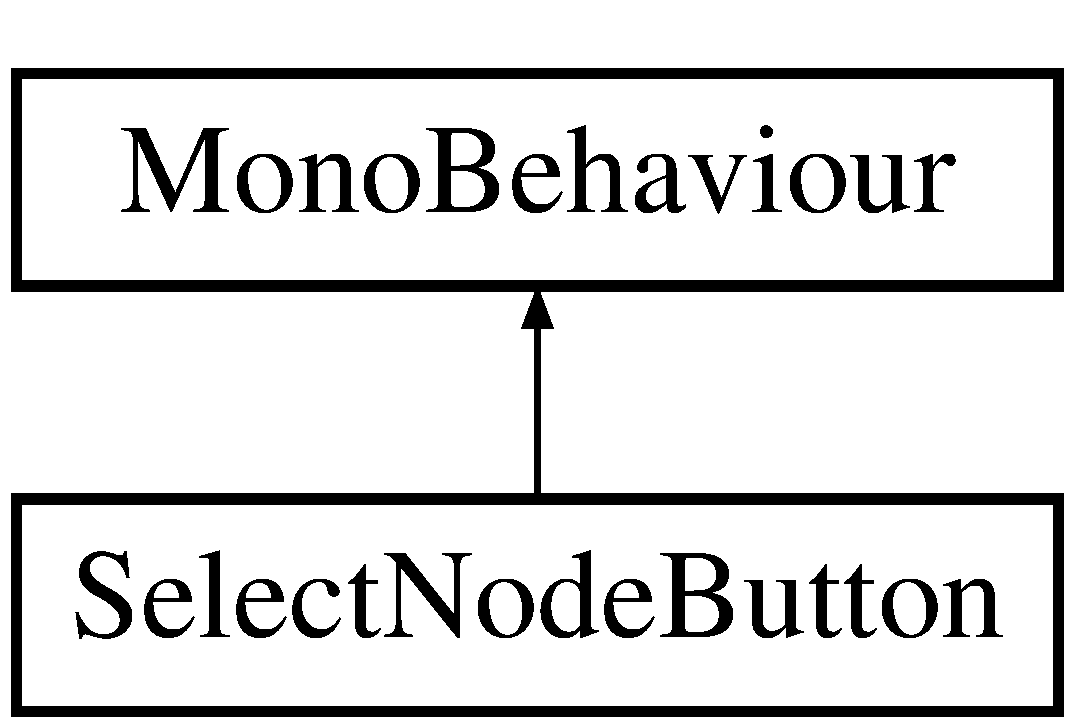
\includegraphics[height=2.000000cm]{class_select_node_button}
\end{center}
\end{figure}
\subsection*{Public Member Functions}
\begin{DoxyCompactItemize}
\item 
void \hyperlink{class_select_node_button_ac0062be5316502f6835aaa2334408bf0}{Deselect} ()
\begin{DoxyCompactList}\small\item\em This node is no longer the selected node. \end{DoxyCompactList}\item 
void \hyperlink{class_select_node_button_a23cb12320f235b9caf63e15c27c100ed}{Change\+Behavior} (Behavior new\+Type)
\begin{DoxyCompactList}\small\item\em Update the behavior of this node \end{DoxyCompactList}\item 
void \hyperlink{class_select_node_button_a0b21ceeb215b5732c7331efa2fb2f434}{Update\+Visuals} ()
\begin{DoxyCompactList}\small\item\em Updates the visuals of this node \end{DoxyCompactList}\item 
void \hyperlink{class_select_node_button_a5c76435d61c0b3bfdc9e6b9ba64f8bc2}{Update\+When} (When new\+Activation)
\begin{DoxyCompactList}\small\item\em Updates the When component of this node. \end{DoxyCompactList}\item 
void \hyperlink{class_select_node_button_af473e0efc29077bd547d6aa39ed5afc0}{Update\+At} (int new\+Number)
\begin{DoxyCompactList}\small\item\em Updates the value of the At component of this node. \end{DoxyCompactList}\item 
void \hyperlink{class_select_node_button_aff33f2066242975f61556b60e2ebcbb1}{Update\+Max} (int new\+Capacity)
\begin{DoxyCompactList}\small\item\em Updates the max value of this node \end{DoxyCompactList}\item 
void \hyperlink{class_select_node_button_a818b654206abd20d9cd47ddb2dd0beaf}{Update\+Act\+How} (Act new\+Act, How new\+How)
\begin{DoxyCompactList}\small\item\em Updates the Act and How values of this node \end{DoxyCompactList}\item 
void \hyperlink{class_select_node_button_a599568299317833815b7f4488f2d0943}{Update\+IO} (IO new\+IO)
\begin{DoxyCompactList}\small\item\em Updates the In Out component of this node. \end{DoxyCompactList}\item 
void \hyperlink{class_select_node_button_aff3ff5c856eda7efdb0509cd09e7930e}{Update\+Add} (string new\+Add)
\begin{DoxyCompactList}\small\item\em Update the add of this node \end{DoxyCompactList}\item 
void \hyperlink{class_select_node_button_a021920607dcc21a0f404e5e31ec4e8f0}{Update\+Of\+Type} (string new\+Of\+Type)
\begin{DoxyCompactList}\small\item\em Updates the Of\+Type of this node (adds a definition) \end{DoxyCompactList}\item 
void \hyperlink{class_select_node_button_a1ff16f5f05301ef738f88fb648ee3c9f}{Update\+Definition\+References} ()
\begin{DoxyCompactList}\small\item\em Updates the node interfaces on this nodes definition \end{DoxyCompactList}\end{DoxyCompactItemize}
\subsection*{Public Attributes}
\begin{DoxyCompactItemize}
\item 
\mbox{\Hypertarget{class_select_node_button_a58072c3259dc5f3e3d65f54e67650e0a}\label{class_select_node_button_a58072c3259dc5f3e3d65f54e67650e0a}} 
Behavior {\bfseries type} = Behavior.\+Pool
\item 
\mbox{\Hypertarget{class_select_node_button_a2ef2cc08df8d5bc9d60e06ea22e260c3}\label{class_select_node_button_a2ef2cc08df8d5bc9d60e06ea22e260c3}} 
Sprite \mbox{[}$\,$\mbox{]} {\bfseries sprites}
\item 
\mbox{\Hypertarget{class_select_node_button_a29542f96105d18dd234da64ac00e65c1}\label{class_select_node_button_a29542f96105d18dd234da64ac00e65c1}} 
Sprite \mbox{[}$\,$\mbox{]} {\bfseries interactible\+Sprites}
\item 
\mbox{\Hypertarget{class_select_node_button_a827121b0c2067f7cf7b12fe19285755f}\label{class_select_node_button_a827121b0c2067f7cf7b12fe19285755f}} 
Sprite \mbox{[}$\,$\mbox{]} {\bfseries inout\+Arrows}
\item 
\mbox{\Hypertarget{class_select_node_button_a01271dc75106b19232d992c02ac17109}\label{class_select_node_button_a01271dc75106b19232d992c02ac17109}} 
Image {\bfseries node\+Image}
\item 
\mbox{\Hypertarget{class_select_node_button_a28775fc91183cdae96b96ccc50851c65}\label{class_select_node_button_a28775fc91183cdae96b96ccc50851c65}} 
Image {\bfseries inout\+Image}
\item 
\mbox{\Hypertarget{class_select_node_button_a549fc8d176d8e385af82537052ae3d0c}\label{class_select_node_button_a549fc8d176d8e385af82537052ae3d0c}} 
bool {\bfseries is\+Selected} = false
\item 
\mbox{\Hypertarget{class_select_node_button_a1bccb3734323a06013825125eaa25f76}\label{class_select_node_button_a1bccb3734323a06013825125eaa25f76}} 
Text {\bfseries label}
\item 
\mbox{\Hypertarget{class_select_node_button_a049422c8d4ef31849400c3c32c4abf37}\label{class_select_node_button_a049422c8d4ef31849400c3c32c4abf37}} 
Text {\bfseries activation\+Text}
\item 
\mbox{\Hypertarget{class_select_node_button_aa2e211cc9a399ff49f50469c4d672c46}\label{class_select_node_button_aa2e211cc9a399ff49f50469c4d672c46}} 
Text {\bfseries pull\+Mode\+Text}
\item 
\mbox{\Hypertarget{class_select_node_button_a1676f7189a3c89fece15d3d5e1f3f76b}\label{class_select_node_button_a1676f7189a3c89fece15d3d5e1f3f76b}} 
Text {\bfseries number\+Text}
\item 
\mbox{\Hypertarget{class_select_node_button_adcca6c09b73e198886b4a24bb129e2e9}\label{class_select_node_button_adcca6c09b73e198886b4a24bb129e2e9}} 
Text {\bfseries max\+Text}
\item 
\mbox{\Hypertarget{class_select_node_button_a5325940983fb34ea299a0e78796b0856}\label{class_select_node_button_a5325940983fb34ea299a0e78796b0856}} 
int {\bfseries number}
\item 
\mbox{\Hypertarget{class_select_node_button_a5dd5ba3c5de34b56b13889177bd2c6dd}\label{class_select_node_button_a5dd5ba3c5de34b56b13889177bd2c6dd}} 
int {\bfseries capacity} = 0
\item 
\mbox{\Hypertarget{class_select_node_button_a5a3b3e58ebe3c605afe985dd259c9810}\label{class_select_node_button_a5a3b3e58ebe3c605afe985dd259c9810}} 
string {\bfseries add} = \char`\"{}\char`\"{}
\item 
\mbox{\Hypertarget{class_select_node_button_ac8e2b8d732c0029d5538212aa96fb342}\label{class_select_node_button_ac8e2b8d732c0029d5538212aa96fb342}} 
string {\bfseries of\+Type} = \char`\"{}\char`\"{}
\item 
\mbox{\Hypertarget{class_select_node_button_a27b39117647cbb0e5eab9d4c7b237a7f}\label{class_select_node_button_a27b39117647cbb0e5eab9d4c7b237a7f}} 
How {\bfseries how} = How.\+Any
\item 
\mbox{\Hypertarget{class_select_node_button_aa7565257f54aac3b000c8a0a0f4031b2}\label{class_select_node_button_aa7565257f54aac3b000c8a0a0f4031b2}} 
Act {\bfseries act} = Act.\+Pull
\item 
\mbox{\Hypertarget{class_select_node_button_abffba7e9b1b50bf3ab09d7ced6da0b1b}\label{class_select_node_button_abffba7e9b1b50bf3ab09d7ced6da0b1b}} 
When {\bfseries when} = When.\+Passive
\item 
\mbox{\Hypertarget{class_select_node_button_a0a2a9f638bcb778c17ef39a238f2fa70}\label{class_select_node_button_a0a2a9f638bcb778c17ef39a238f2fa70}} 
IO {\bfseries inout} = I\+O.\+Internal
\item 
\mbox{\Hypertarget{class_select_node_button_a0ea1ac3e82cb50ab25b2051cec1eea1f}\label{class_select_node_button_a0ea1ac3e82cb50ab25b2051cec1eea1f}} 
Game\+Object {\bfseries definition} = null
\item 
\mbox{\Hypertarget{class_select_node_button_a00975033c812896a53573bcd22f5fd70}\label{class_select_node_button_a00975033c812896a53573bcd22f5fd70}} 
Game\+Object {\bfseries definition\+Prefab}
\item 
\mbox{\Hypertarget{class_select_node_button_a556f26b91242f1c4752d9de59d543769}\label{class_select_node_button_a556f26b91242f1c4752d9de59d543769}} 
bool {\bfseries drag} = false
\item 
\mbox{\Hypertarget{class_select_node_button_a5616b1a16ea0dfa6faea73a8e3a742eb}\label{class_select_node_button_a5616b1a16ea0dfa6faea73a8e3a742eb}} 
M\+M.\+Model.\+Node {\bfseries id\+Node} = null
\end{DoxyCompactItemize}


\subsection{Detailed Description}
Stores and updates the visual elements of a node 



\subsection{Member Function Documentation}
\mbox{\Hypertarget{class_select_node_button_a23cb12320f235b9caf63e15c27c100ed}\label{class_select_node_button_a23cb12320f235b9caf63e15c27c100ed}} 
\index{Select\+Node\+Button@{Select\+Node\+Button}!Change\+Behavior@{Change\+Behavior}}
\index{Change\+Behavior@{Change\+Behavior}!Select\+Node\+Button@{Select\+Node\+Button}}
\subsubsection{\texorpdfstring{Change\+Behavior()}{ChangeBehavior()}}
{\footnotesize\ttfamily void Select\+Node\+Button.\+Change\+Behavior (\begin{DoxyParamCaption}\item[{Behavior}]{new\+Type }\end{DoxyParamCaption})}



Update the behavior of this node 


\begin{DoxyParams}{Parameters}
{\em new\+Type} & the new behavior \\
\hline
\end{DoxyParams}
\mbox{\Hypertarget{class_select_node_button_ac0062be5316502f6835aaa2334408bf0}\label{class_select_node_button_ac0062be5316502f6835aaa2334408bf0}} 
\index{Select\+Node\+Button@{Select\+Node\+Button}!Deselect@{Deselect}}
\index{Deselect@{Deselect}!Select\+Node\+Button@{Select\+Node\+Button}}
\subsubsection{\texorpdfstring{Deselect()}{Deselect()}}
{\footnotesize\ttfamily void Select\+Node\+Button.\+Deselect (\begin{DoxyParamCaption}{ }\end{DoxyParamCaption})}



This node is no longer the selected node. 

\mbox{\Hypertarget{class_select_node_button_a818b654206abd20d9cd47ddb2dd0beaf}\label{class_select_node_button_a818b654206abd20d9cd47ddb2dd0beaf}} 
\index{Select\+Node\+Button@{Select\+Node\+Button}!Update\+Act\+How@{Update\+Act\+How}}
\index{Update\+Act\+How@{Update\+Act\+How}!Select\+Node\+Button@{Select\+Node\+Button}}
\subsubsection{\texorpdfstring{Update\+Act\+How()}{UpdateActHow()}}
{\footnotesize\ttfamily void Select\+Node\+Button.\+Update\+Act\+How (\begin{DoxyParamCaption}\item[{Act}]{new\+Act,  }\item[{How}]{new\+How }\end{DoxyParamCaption})}



Updates the Act and How values of this node 


\begin{DoxyParams}{Parameters}
{\em new\+Act} & new Act of this node \\
\hline
{\em new\+How} & new How of this node \\
\hline
\end{DoxyParams}
\mbox{\Hypertarget{class_select_node_button_aff3ff5c856eda7efdb0509cd09e7930e}\label{class_select_node_button_aff3ff5c856eda7efdb0509cd09e7930e}} 
\index{Select\+Node\+Button@{Select\+Node\+Button}!Update\+Add@{Update\+Add}}
\index{Update\+Add@{Update\+Add}!Select\+Node\+Button@{Select\+Node\+Button}}
\subsubsection{\texorpdfstring{Update\+Add()}{UpdateAdd()}}
{\footnotesize\ttfamily void Select\+Node\+Button.\+Update\+Add (\begin{DoxyParamCaption}\item[{string}]{new\+Add }\end{DoxyParamCaption})}



Update the add of this node 


\begin{DoxyParams}{Parameters}
{\em new\+Add} & new add value of this node \\
\hline
\end{DoxyParams}
\mbox{\Hypertarget{class_select_node_button_af473e0efc29077bd547d6aa39ed5afc0}\label{class_select_node_button_af473e0efc29077bd547d6aa39ed5afc0}} 
\index{Select\+Node\+Button@{Select\+Node\+Button}!Update\+At@{Update\+At}}
\index{Update\+At@{Update\+At}!Select\+Node\+Button@{Select\+Node\+Button}}
\subsubsection{\texorpdfstring{Update\+At()}{UpdateAt()}}
{\footnotesize\ttfamily void Select\+Node\+Button.\+Update\+At (\begin{DoxyParamCaption}\item[{int}]{new\+Number }\end{DoxyParamCaption})}



Updates the value of the At component of this node. 


\begin{DoxyParams}{Parameters}
{\em new\+Number} & the new number \\
\hline
\end{DoxyParams}
\mbox{\Hypertarget{class_select_node_button_a1ff16f5f05301ef738f88fb648ee3c9f}\label{class_select_node_button_a1ff16f5f05301ef738f88fb648ee3c9f}} 
\index{Select\+Node\+Button@{Select\+Node\+Button}!Update\+Definition\+References@{Update\+Definition\+References}}
\index{Update\+Definition\+References@{Update\+Definition\+References}!Select\+Node\+Button@{Select\+Node\+Button}}
\subsubsection{\texorpdfstring{Update\+Definition\+References()}{UpdateDefinitionReferences()}}
{\footnotesize\ttfamily void Select\+Node\+Button.\+Update\+Definition\+References (\begin{DoxyParamCaption}{ }\end{DoxyParamCaption})}



Updates the node interfaces on this nodes definition 

\mbox{\Hypertarget{class_select_node_button_a599568299317833815b7f4488f2d0943}\label{class_select_node_button_a599568299317833815b7f4488f2d0943}} 
\index{Select\+Node\+Button@{Select\+Node\+Button}!Update\+IO@{Update\+IO}}
\index{Update\+IO@{Update\+IO}!Select\+Node\+Button@{Select\+Node\+Button}}
\subsubsection{\texorpdfstring{Update\+I\+O()}{UpdateIO()}}
{\footnotesize\ttfamily void Select\+Node\+Button.\+Update\+IO (\begin{DoxyParamCaption}\item[{IO}]{new\+IO }\end{DoxyParamCaption})}



Updates the In Out component of this node. 


\begin{DoxyParams}{Parameters}
{\em new\+IO} & new In Out of this node \\
\hline
\end{DoxyParams}
\mbox{\Hypertarget{class_select_node_button_aff33f2066242975f61556b60e2ebcbb1}\label{class_select_node_button_aff33f2066242975f61556b60e2ebcbb1}} 
\index{Select\+Node\+Button@{Select\+Node\+Button}!Update\+Max@{Update\+Max}}
\index{Update\+Max@{Update\+Max}!Select\+Node\+Button@{Select\+Node\+Button}}
\subsubsection{\texorpdfstring{Update\+Max()}{UpdateMax()}}
{\footnotesize\ttfamily void Select\+Node\+Button.\+Update\+Max (\begin{DoxyParamCaption}\item[{int}]{new\+Capacity }\end{DoxyParamCaption})}



Updates the max value of this node 


\begin{DoxyParams}{Parameters}
{\em new\+Capacity} & the new max value, a max of 0 means there is no max \\
\hline
\end{DoxyParams}
\mbox{\Hypertarget{class_select_node_button_a021920607dcc21a0f404e5e31ec4e8f0}\label{class_select_node_button_a021920607dcc21a0f404e5e31ec4e8f0}} 
\index{Select\+Node\+Button@{Select\+Node\+Button}!Update\+Of\+Type@{Update\+Of\+Type}}
\index{Update\+Of\+Type@{Update\+Of\+Type}!Select\+Node\+Button@{Select\+Node\+Button}}
\subsubsection{\texorpdfstring{Update\+Of\+Type()}{UpdateOfType()}}
{\footnotesize\ttfamily void Select\+Node\+Button.\+Update\+Of\+Type (\begin{DoxyParamCaption}\item[{string}]{new\+Of\+Type }\end{DoxyParamCaption})}



Updates the Of\+Type of this node (adds a definition) 


\begin{DoxyParams}{Parameters}
{\em new\+Of\+Type} & new Of\+Type \\
\hline
\end{DoxyParams}
\mbox{\Hypertarget{class_select_node_button_a0b21ceeb215b5732c7331efa2fb2f434}\label{class_select_node_button_a0b21ceeb215b5732c7331efa2fb2f434}} 
\index{Select\+Node\+Button@{Select\+Node\+Button}!Update\+Visuals@{Update\+Visuals}}
\index{Update\+Visuals@{Update\+Visuals}!Select\+Node\+Button@{Select\+Node\+Button}}
\subsubsection{\texorpdfstring{Update\+Visuals()}{UpdateVisuals()}}
{\footnotesize\ttfamily void Select\+Node\+Button.\+Update\+Visuals (\begin{DoxyParamCaption}{ }\end{DoxyParamCaption})}



Updates the visuals of this node 

\mbox{\Hypertarget{class_select_node_button_a5c76435d61c0b3bfdc9e6b9ba64f8bc2}\label{class_select_node_button_a5c76435d61c0b3bfdc9e6b9ba64f8bc2}} 
\index{Select\+Node\+Button@{Select\+Node\+Button}!Update\+When@{Update\+When}}
\index{Update\+When@{Update\+When}!Select\+Node\+Button@{Select\+Node\+Button}}
\subsubsection{\texorpdfstring{Update\+When()}{UpdateWhen()}}
{\footnotesize\ttfamily void Select\+Node\+Button.\+Update\+When (\begin{DoxyParamCaption}\item[{When}]{new\+Activation }\end{DoxyParamCaption})}



Updates the When component of this node. 


\begin{DoxyParams}{Parameters}
{\em new\+Activation} & the new When \\
\hline
\end{DoxyParams}


The documentation for this class was generated from the following file\+:\begin{DoxyCompactItemize}
\item 
Select\+Node\+Button.\+cs\end{DoxyCompactItemize}

\hypertarget{class_tab_manager}{}\section{Tab\+Manager Class Reference}
\label{class_tab_manager}\index{Tab\+Manager@{Tab\+Manager}}


Script that manages the tabs and adds new tabs  


Inheritance diagram for Tab\+Manager\+:\begin{figure}[H]
\begin{center}
\leavevmode
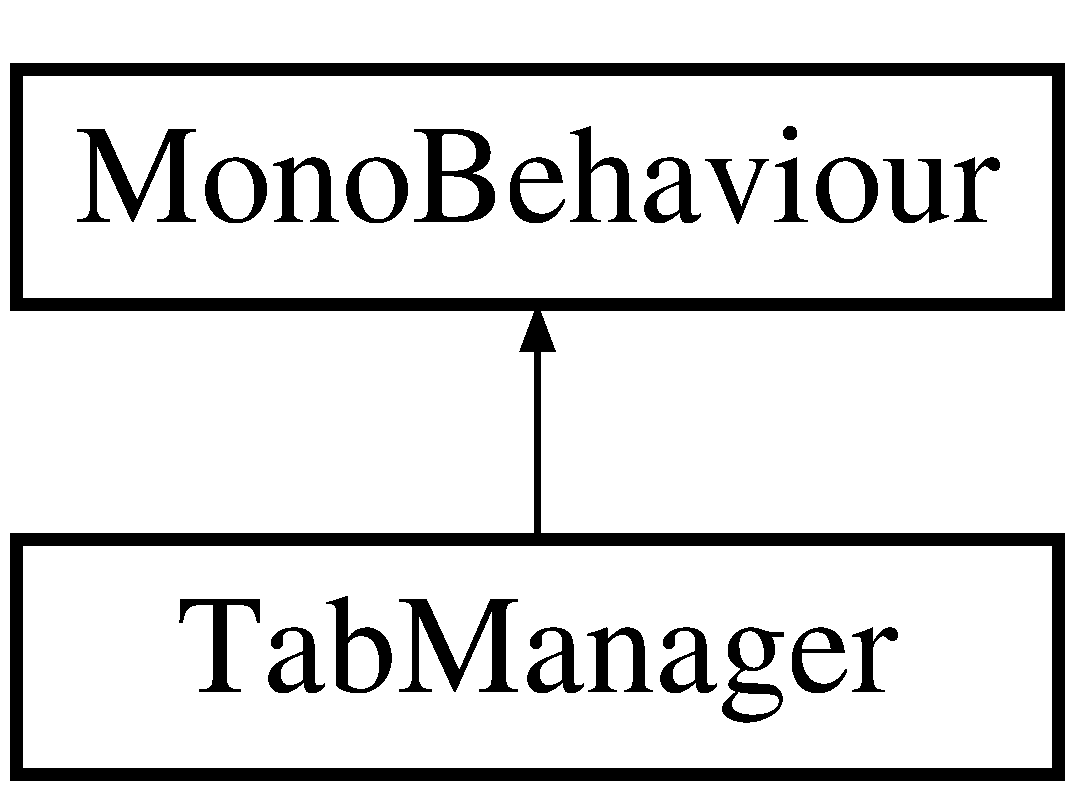
\includegraphics[height=2.000000cm]{class_tab_manager}
\end{center}
\end{figure}
\subsection*{Public Member Functions}
\begin{DoxyCompactItemize}
\item 
void \hyperlink{class_tab_manager_addabe80f37af16c101517e0a4c63fdef}{Add\+Tab} (string name)
\begin{DoxyCompactList}\small\item\em Adds a tab to the diagram \end{DoxyCompactList}\item 
void \hyperlink{class_tab_manager_a060b949fab08f226d44b0daa86e5c424}{Tab\+Removed} ()
\begin{DoxyCompactList}\small\item\em When this script receives a \char`\"{}tab\+Removed\char`\"{} event this function scales the remaining tabs up \end{DoxyCompactList}\item 
Game\+Object \hyperlink{class_tab_manager_a98d132c5a132278fad057a17463f0000}{Get\+Last\+Tab} ()
\begin{DoxyCompactList}\small\item\em returns the active tab \end{DoxyCompactList}\end{DoxyCompactItemize}
\subsection*{Public Attributes}
\begin{DoxyCompactItemize}
\item 
\mbox{\Hypertarget{class_tab_manager_a4da840c069f5dbdff9e99072b892853a}\label{class_tab_manager_a4da840c069f5dbdff9e99072b892853a}} 
Button {\bfseries your\+Button}
\item 
\mbox{\Hypertarget{class_tab_manager_ac948c833bf1af52a2b6fe0329633b5de}\label{class_tab_manager_ac948c833bf1af52a2b6fe0329633b5de}} 
Game\+Object {\bfseries graph\+Tab}
\item 
\mbox{\Hypertarget{class_tab_manager_ac5766310834b7c9266c4f8ebdd3e094e}\label{class_tab_manager_ac5766310834b7c9266c4f8ebdd3e094e}} 
Transform {\bfseries canvas}
\item 
\mbox{\Hypertarget{class_tab_manager_a4e2bfa11e6d027771976694f5d7031a7}\label{class_tab_manager_a4e2bfa11e6d027771976694f5d7031a7}} 
int {\bfseries tab\+Count} = 0
\item 
\mbox{\Hypertarget{class_tab_manager_a5ef5fb0116c9331f3df7e4e2b7dc4099}\label{class_tab_manager_a5ef5fb0116c9331f3df7e4e2b7dc4099}} 
Game\+Object {\bfseries temp\+Obj}
\item 
\mbox{\Hypertarget{class_tab_manager_a9b81c8d17fb6fba80bbbbc9fe7d66efc}\label{class_tab_manager_a9b81c8d17fb6fba80bbbbc9fe7d66efc}} 
float {\bfseries scale} = 1.\+0f
\item 
\mbox{\Hypertarget{class_tab_manager_aa946d34ac37a73032a4f8b9eb7d5eddb}\label{class_tab_manager_aa946d34ac37a73032a4f8b9eb7d5eddb}} 
int {\bfseries name\+Counter} = 1
\item 
\mbox{\Hypertarget{class_tab_manager_a856215722f62956293ae49169e8511e2}\label{class_tab_manager_a856215722f62956293ae49169e8511e2}} 
\hyperlink{class_model_controller}{Model\+Controller} {\bfseries model}
\end{DoxyCompactItemize}


\subsection{Detailed Description}
Script that manages the tabs and adds new tabs 



\subsection{Member Function Documentation}
\mbox{\Hypertarget{class_tab_manager_addabe80f37af16c101517e0a4c63fdef}\label{class_tab_manager_addabe80f37af16c101517e0a4c63fdef}} 
\index{Tab\+Manager@{Tab\+Manager}!Add\+Tab@{Add\+Tab}}
\index{Add\+Tab@{Add\+Tab}!Tab\+Manager@{Tab\+Manager}}
\subsubsection{\texorpdfstring{Add\+Tab()}{AddTab()}}
{\footnotesize\ttfamily void Tab\+Manager.\+Add\+Tab (\begin{DoxyParamCaption}\item[{string}]{name }\end{DoxyParamCaption})}



Adds a tab to the diagram 


\begin{DoxyParams}{Parameters}
{\em name} & name of the new tab\\
\hline
\end{DoxyParams}
\mbox{\Hypertarget{class_tab_manager_a98d132c5a132278fad057a17463f0000}\label{class_tab_manager_a98d132c5a132278fad057a17463f0000}} 
\index{Tab\+Manager@{Tab\+Manager}!Get\+Last\+Tab@{Get\+Last\+Tab}}
\index{Get\+Last\+Tab@{Get\+Last\+Tab}!Tab\+Manager@{Tab\+Manager}}
\subsubsection{\texorpdfstring{Get\+Last\+Tab()}{GetLastTab()}}
{\footnotesize\ttfamily Game\+Object Tab\+Manager.\+Get\+Last\+Tab (\begin{DoxyParamCaption}{ }\end{DoxyParamCaption})}



returns the active tab 

\begin{DoxyReturn}{Returns}
Returns the active tab
\end{DoxyReturn}
\mbox{\Hypertarget{class_tab_manager_a060b949fab08f226d44b0daa86e5c424}\label{class_tab_manager_a060b949fab08f226d44b0daa86e5c424}} 
\index{Tab\+Manager@{Tab\+Manager}!Tab\+Removed@{Tab\+Removed}}
\index{Tab\+Removed@{Tab\+Removed}!Tab\+Manager@{Tab\+Manager}}
\subsubsection{\texorpdfstring{Tab\+Removed()}{TabRemoved()}}
{\footnotesize\ttfamily void Tab\+Manager.\+Tab\+Removed (\begin{DoxyParamCaption}{ }\end{DoxyParamCaption})}



When this script receives a \char`\"{}tab\+Removed\char`\"{} event this function scales the remaining tabs up 



The documentation for this class was generated from the following file\+:\begin{DoxyCompactItemize}
\item 
Tab\+Manager.\+cs\end{DoxyCompactItemize}

\hypertarget{class_tab_text}{}\section{Tab\+Text Class Reference}
\label{class_tab_text}\index{Tab\+Text@{Tab\+Text}}


This script disables the input field of the tab unless it is the active tab.  


Inheritance diagram for Tab\+Text\+:\begin{figure}[H]
\begin{center}
\leavevmode
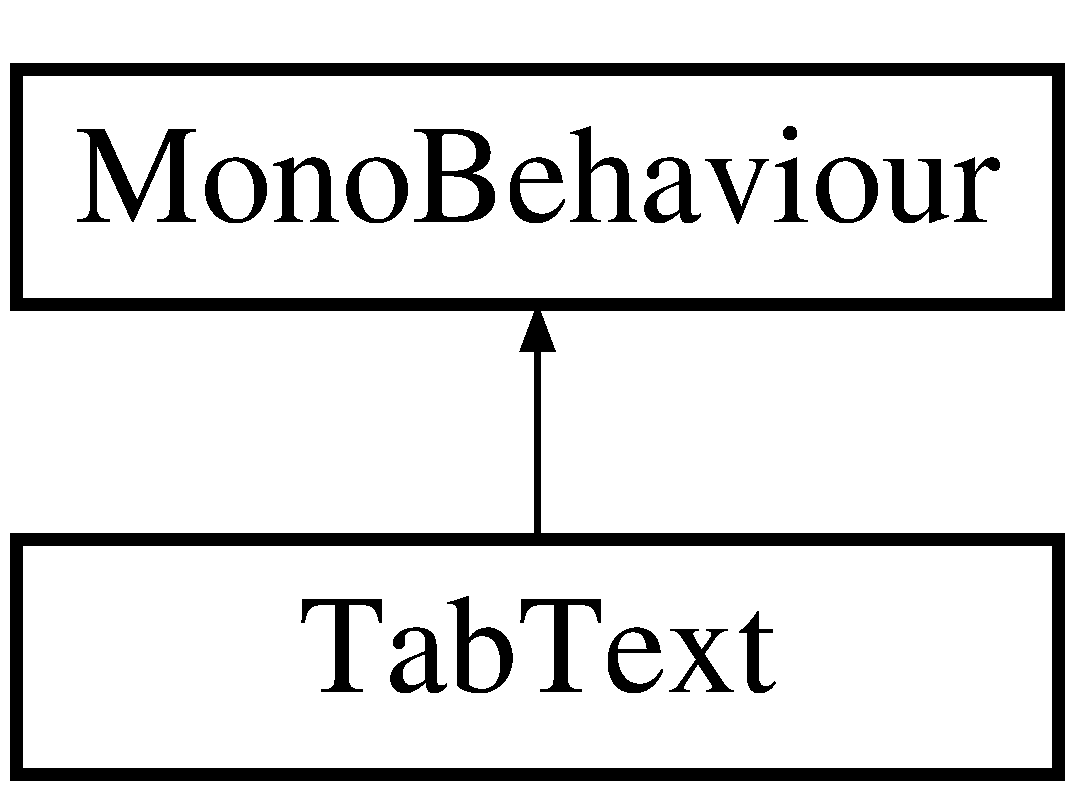
\includegraphics[height=2.000000cm]{class_tab_text}
\end{center}
\end{figure}
\subsection*{Public Member Functions}
\begin{DoxyCompactItemize}
\item 
void \hyperlink{class_tab_text_a10061d722257289b90501c8251fa2d1a}{Update\+Definition} ()
\begin{DoxyCompactList}\small\item\em Updates the definition name in the model \end{DoxyCompactList}\end{DoxyCompactItemize}
\subsection*{Public Attributes}
\begin{DoxyCompactItemize}
\item 
\mbox{\Hypertarget{class_tab_text_aaa83367064d26906556fb752b7c4fbd7}\label{class_tab_text_aaa83367064d26906556fb752b7c4fbd7}} 
Game\+Object {\bfseries parent}
\item 
\mbox{\Hypertarget{class_tab_text_af59e01ebf1860ac451b686d5fd51e8af}\label{class_tab_text_af59e01ebf1860ac451b686d5fd51e8af}} 
Input\+Field {\bfseries ipf}
\item 
\mbox{\Hypertarget{class_tab_text_ada044dfae3469e4db4845e24c140cdfb}\label{class_tab_text_ada044dfae3469e4db4845e24c140cdfb}} 
string {\bfseries old\+Name}
\item 
\mbox{\Hypertarget{class_tab_text_a49910f80dd10d636e8c96e0f99897e27}\label{class_tab_text_a49910f80dd10d636e8c96e0f99897e27}} 
string {\bfseries new\+Name}
\item 
\mbox{\Hypertarget{class_tab_text_ac3068749828c914f91f3952a85441196}\label{class_tab_text_ac3068749828c914f91f3952a85441196}} 
\hyperlink{class_model_controller}{Model\+Controller} {\bfseries model}
\end{DoxyCompactItemize}


\subsection{Detailed Description}
This script disables the input field of the tab unless it is the active tab. 



\subsection{Member Function Documentation}
\mbox{\Hypertarget{class_tab_text_a10061d722257289b90501c8251fa2d1a}\label{class_tab_text_a10061d722257289b90501c8251fa2d1a}} 
\index{Tab\+Text@{Tab\+Text}!Update\+Definition@{Update\+Definition}}
\index{Update\+Definition@{Update\+Definition}!Tab\+Text@{Tab\+Text}}
\subsubsection{\texorpdfstring{Update\+Definition()}{UpdateDefinition()}}
{\footnotesize\ttfamily void Tab\+Text.\+Update\+Definition (\begin{DoxyParamCaption}{ }\end{DoxyParamCaption})}



Updates the definition name in the model 



The documentation for this class was generated from the following file\+:\begin{DoxyCompactItemize}
\item 
Tab\+Text.\+cs\end{DoxyCompactItemize}

\hypertarget{class_toggle_tool}{}\section{Toggle\+Tool Class Reference}
\label{class_toggle_tool}\index{Toggle\+Tool@{Toggle\+Tool}}


This script manages the tool enabling and disabling (toggling)  


Inheritance diagram for Toggle\+Tool\+:\begin{figure}[H]
\begin{center}
\leavevmode
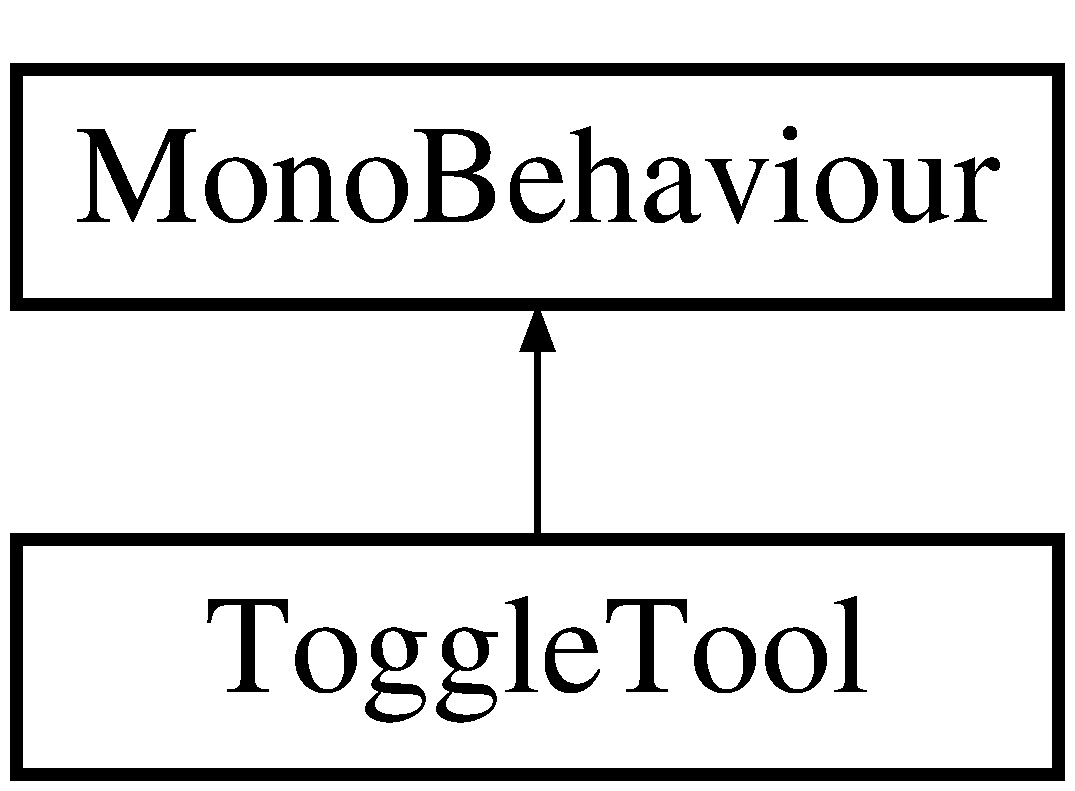
\includegraphics[height=2.000000cm]{class_toggle_tool}
\end{center}
\end{figure}
\subsection*{Public Member Functions}
\begin{DoxyCompactItemize}
\item 
\mbox{\Hypertarget{class_toggle_tool_ac762d14aa1b31efbf98c87b1dd01e7f7}\label{class_toggle_tool_ac762d14aa1b31efbf98c87b1dd01e7f7}} 
void {\bfseries Handle\+On\+Exit} ()
\end{DoxyCompactItemize}
\subsection*{Public Attributes}
\begin{DoxyCompactItemize}
\item 
\mbox{\Hypertarget{class_toggle_tool_a7a098df27a26933369a7689fddc76d29}\label{class_toggle_tool_a7a098df27a26933369a7689fddc76d29}} 
bool {\bfseries tool\+Enabled} = true
\end{DoxyCompactItemize}


\subsection{Detailed Description}
This script manages the tool enabling and disabling (toggling) 



The documentation for this class was generated from the following file\+:\begin{DoxyCompactItemize}
\item 
Toggle\+Tool.\+cs\end{DoxyCompactItemize}

\hypertarget{class_zoom_content_script}{}\section{Zoom\+Content\+Script Class Reference}
\label{class_zoom_content_script}\index{Zoom\+Content\+Script@{Zoom\+Content\+Script}}


This script enables the user to use the scroll wheel to zoom out on diagrams  


Inheritance diagram for Zoom\+Content\+Script\+:\begin{figure}[H]
\begin{center}
\leavevmode
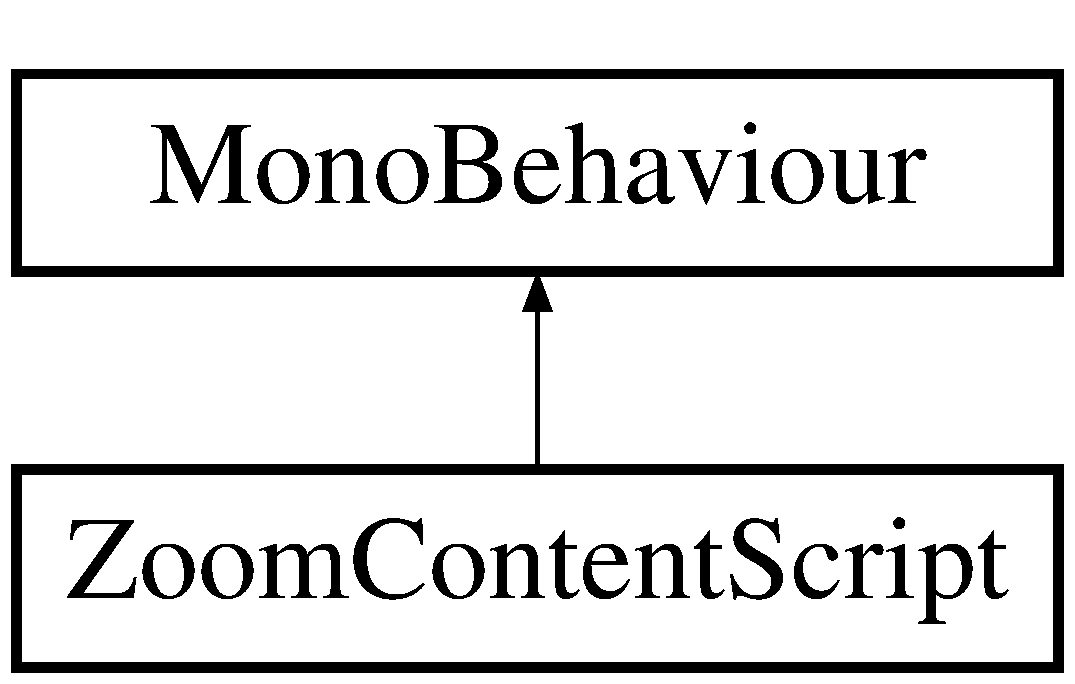
\includegraphics[height=2.000000cm]{class_zoom_content_script}
\end{center}
\end{figure}
\subsection*{Public Attributes}
\begin{DoxyCompactItemize}
\item 
\mbox{\Hypertarget{class_zoom_content_script_a69e4b0a49e6ad07efd2d1f1880b4afca}\label{class_zoom_content_script_a69e4b0a49e6ad07efd2d1f1880b4afca}} 
Rect\+Transform {\bfseries content}
\item 
\mbox{\Hypertarget{class_zoom_content_script_a9bb6fa3258f3c8017614105a3b3a5a2d}\label{class_zoom_content_script_a9bb6fa3258f3c8017614105a3b3a5a2d}} 
Transform {\bfseries canvas}
\item 
\mbox{\Hypertarget{class_zoom_content_script_a3dff555225fc47347dd914f4d09f57ae}\label{class_zoom_content_script_a3dff555225fc47347dd914f4d09f57ae}} 
Transform {\bfseries grid}
\end{DoxyCompactItemize}


\subsection{Detailed Description}
This script enables the user to use the scroll wheel to zoom out on diagrams 



The documentation for this class was generated from the following file\+:\begin{DoxyCompactItemize}
\item 
Zoom\+Content\+Script.\+cs\end{DoxyCompactItemize}

%--- End generated contents ---

% Index
\backmatter
\newpage
\phantomsection
\clearemptydoublepage
\addcontentsline{toc}{chapter}{Index}
\printindex

\end{document}
